%-*- coding: UTF-8 -*-

\documentclass[zihao=5, sub3section, UTF8, fontset=windows, scheme=plain, punct]{ctexart} % ctex documentclasses include ctexart, ctexrep and ctexbook
% \documentclass[a4paper, landscape, oneside, 10pt, 
%                 onecolumn, titlepage, openany, leqno, fleqn, 
%                 draft, openbib]{article}   % latex basic document classes include article, report and book
% by default, letterpaper, no landscape item, oneside, 10pt, 
%               onecolumn, notitlepage, openany, no leqno item, no fleqn item, 
%               final, no openbib item

%%%%%%%%%%---------- Fonts ----------%%%%%%%%%%
% \usepackage{amsthm}                     % for using some theorem environment, must before fontspec, incompatible with ntheorem

% \frenchspacing                          % for forbidding extra blank after puctuations, only the same blank length between the normal words
% \CJKsetecglue{}                         % for forbidding auto-blank between chinese and other contents completely
% \renewcommand\nocorrlist{,.A}           % for not correcting the specific characters' slanted overflow

\usepackage{fontspec}                   % for using xetex setting font family, if `no-math`, then no influencing the math font
\setmainfont{Times New Roman}
\setsansfont{Verdana}
\setmonofont{Courier New}
\newfontfamily\lucidasans{Lucida Sans}  % for define new font family, used by \lucidasans
\setmathrm{Latin Modern Math}
\setmathsf{Verdana}
\setmathtt{Courier New}

\newcommand\Emph{\textbf}               % for defining more emphasize, used by \Emph
\usepackage[normalem]{ulem}             % for correct underline, if `normalem`, then no influencing the \emph, used by \uline
\usepackage{xeCJKfntef}                 % for using underline chinese, if `normalem`, then no influencing the \emph

\setCJKmainfont{SimSun}
\setCJKsansfont{YouYuan}
\setCJKmonofont{FangSong}
\setCJKfamilyfont{kai}{KaiTi}           % for defining new chinese font family, used by \CJKfamily{kai}

\linespread{1}                          % set line spacing
\selectfont

%%%%%%%%%%---------- Blank ----------%%%%%%%%%%
\newlength\mylen                        % define own length variable
\setlength\mylen{2em}

%%%%%%%%%%---------- Box ----------%%%%%%%%%%
\newsavebox\mybox                       % define own box variable, used by \mybox
\sbox\mybox{My box contents}
\savebox\mybox[5cm][s]{My box contents} % c for center, l for left, r for right, s for stretched
% \usepackage{varwidth}
% \usepackage{graphicx}

%%%%%%%%%%---------- Paragraph ----------%%%%%%%%%%
\usepackage{indentfirst}                % for setting paragraph indent
\setlength{\parindent}{2em}

\hyphenation{man-u-script com-pu-ter}   % manuscript set the hyphenation

\usepackage{ragged2e}                   % for paragraph setting's supplement

\usepackage{microtype}                  % for better english uneven short lines, just included, no need to use explicitly

\usepackage{lettrine}                   % for first word sanking, used by \lettrine

\usepackage{shapepar}                   % for editing the paragraph shape

%%%%%%%%%%---------- Word Environment ----------%%%%%%%%%%
\renewcommand\abstractname{Name for abstract}   % for renaming the title of abstract
\ctexset{abstractname={Name for abstract}}      % for renaming the title of abstract in Chinese

%%%%%%%%%%---------- List ----------%%%%%%%%%%
\renewcommand\theenumii{\fnsymbol{enumii}}      % for changing the index of enumerate environment
\renewcommand\labelenumii{(\theenumii)}         % for changing the tag of enumerate environment, similar for itemize environment

\newenvironment{myitemize}{%
    \begin{list}{\textbullet}{%
        \setlength\topsep{0pt} \setlength\partopsep{0pt} \setlength\parsep{0pt} \setlength\itemsep{0pt}}}
    {\end{list}}                                % general list difficult to use, often used for new own environment

\usepackage{enumitem}                           % for editting easily enumerate environment
\AddEnumerateCounter{\chinese}{\chinese}{}      % for processing no-standard counter

%%%%%%%%%%---------- Counter ----------%%%%%%%%%%
\newcounter{mycnt}[section]                     % for defining own counter variable, if added another counter, then that counter step will cause mycnt clear
\setcounter{mycnt}{0}
\renewcommand\themycnt{\thesection-\arabic{mycnt}}
% used by \stepcounter{mycnt}\themycnt, \addtocounter{mycnt}{-1}\themycnt, often as part of own defined command

\usepackage[centertags, sumlimits, nointlimits, namelimits]{amsmath}
% centertags or tbtags, sumlimits or nosumlimits, intlimits or nointlimits, namelimits or nonamelimits
\numberwithin{equation}{section}                % for making equation indexing along with section

\usepackage{chngcntr}                           % similar to amsmath
\counterwithin{figure}{section}                 % for making figure indexing along with section
\counterwithout{figure}{section}                % for making figure indexing not along with section

%%%%%%%%%%---------- Theorem ----------%%%%%%%%%%
% \usepackage{theorem}                            % for changing the style of theorem environment, must above newtheorem
\usepackage[thmmarks]{ntheorem}                 % better than theorem, added theoremstyle nonumberplain, nonumberbreak, empty, if `thmmarks`, then can use \theoremsymbol
\theoremstyle{plain}                            % also plain, break, marginbreak, changebreak, change, margin
\theoremheaderfont{\sffamily\bfseries}
\theorembodyfont{\normalfont}
\setlength\theorempreskipamount{5pt}
\setlength\theorempostskipamount{5pt}
\theoremsymbol{\ensuremath{\boxed{\phantom{n}}}}

% \usepackage{amsthm}
% \renewcommand\proofname{ProofTitle}             % used by \begin{proof}
% \renewcommand\qedsymbol{\ensuremath{\boxed{\phantom{M}}}}

\newtheorem{thm}{TheoremTitle}[section]         % for creating a new theorem environment, used by \begin{thm}, if added another counter, then that counter step will cause thm clear
% if the counter is located in the middle, then the index is determined by the counter, often used for different theorem with same index

%%%%%%%%%%---------- Verbatim ----------%%%%%%%%%%
\newsavebox\verbbox                             % used for verbatim
\begin{lrbox}\verbbox
    \verb!#$%^&{}!
\end{lrbox}

\newsavebox\verbatimbox                         % used for verbatim multiple lines
\begin{lrbox}\verbatimbox
    \begin{minipage}{10em}
        \begin{verbatim}
            #$%^&{}
            #$%^&{}
            #$%^&{}
        \end{verbatim}
    \end{minipage}
\end{lrbox}

\usepackage{fancyvrb}                           % used for verbatim
\SaveVerb{myverb}!#^&{}!                        % used by \UseVerb

\usepackage{cprotect}                           % for protecting verbatim as other commands' parameter

\usepackage{verbatim}                           % for verbatiming whole file

\usepackage{shortvrb}                           % for short writing the verbatim
% \MakeShortVerb!                                 % used by directly !something!, danger to some degree

%%%%%%%%%%---------- Codes ----------%%%%%%%%%%
\usepackage{listings}                           % for codes environment, used by \begin{lstlisting}
\lstset{
    basicstyle=\sffamily,
    keywordstyle=\bfseries,
    commentstyle=\rmfamily\itshape,
    stringstyle=\ttfamily,
    flexiblecolumns,                            % same as columns=flexible
    numbers=left, numberstyle=\footnotesize,
    escapechar=`,
    language=C
}

%%%%%%%%%%---------- Tabular ----------%%%%%%%%%%
\usepackage{dcolumn}                            % for using tabular aligned with math dot, will also usepackage array by default
\newcolumntype{d}{D{.}{.}{2}}                   % for changing the use of math dot, input as ., output as ., allow 2 bits

\setlength\tabcolsep{1em}                       % for changing the length between columns in tabular
\setlength\arraycolsep{1em}                     % for changing the length between columns in array
\renewcommand\arraystretch{2}                   % for changing the length between rows in tabular and array, by default 1

% \usepackage{array}                              % already include by default with dcolumn

\usepackage{multirow}                           % for using multirow tabular

\usepackage{rotating, makecell}                 % for using tabular item cell

\usepackage{diagbox}                            % for using diagnal tabular item

\usepackage{tabularx}                           % for using fixed width tabular, used by \begin{tabularx}
\newcolumntype{Y}{>{\centering\arraybackslash}X}    % for changing the style of tabularx

\usepackage{longtable}                          % for using long tabular, used by \begin{longtable}

\usepackage{ltxtable}                           % for using long tabular with tabularx, used by \LTXtable

\usepackage[delarray]{tabu}                     % for using tabular more easily, must also together with longtable

\usepackage{xtab}                               % for using long tabular also, used by \begin{xtabular} or \begin{xtabular*}

\usepackage{booktabs}                           % for using different thickness tabular line, almost for three-line table
\setlength\heavyrulewidth{0.08em}               % for changing the thickness of \toprule and \bottomrule
\setlength\lightrulewidth{0.05em}               % for changing the thickness of \midrule
\setlength\cmidrulewidth{0.03em}                % for changing the thickness of \cmidrule
\setlength\aboverulesep{0.03em}                 % for changing the length above \bottomrule and \midrule and \cmidrule
\setlength\belowrulesep{0.03em}                 % for changing the length below \toprule and \midrule and \cmidrule
\setlength\abovetopsep{0em}                     % for changing the length above \toprule
\setlength\belowbottomsep{0em}                  % for changing the length below \bottomrule

\setlength\arrayrulewidth{1pt}                  % for changing the whole lines thichness in tabular

\newcolumntype{v}{!{\vrule width 2pt}}          % for using different thickness vertical lines in tabular

\setlength\doublerulesep{1pt}                   % for changing the length between double lines in tabular

\usepackage{hhline}                             % for using correct double lines in tabular

% \usepackage{arydshln}                           % for using dash line in tabular, conflict with hhline and makecell
% \newcolumntype{|}{!{\vline}}                    % for solving the conflict between arydshln and hhline, makecell, bug exists

% \setlength\dashlinedash{4pt}                    % for changing the length of dash in dash line in tabular
% \setlength\dashlinegap{4pt}                     % for changing the length of gap in dash line in tabular

\usepackage{rotfloat}                           % for using rotated table and figure, used by \begin{sidewaystable} and \begin{sidewaysfigure}

\usepackage{caption, subcaption}                % for changing the style of the caption of float
\captionsetup[table]{format=hang, labelformat=brace, labelsep=endash, justification=centering, singlelinecheck=false, 
                    font={small,sf}, labelfont=sc, textfont=bf, width=20em, skip=10pt, name=TableName}
\usepackage{bicaption}                          % for using bilingual caption
\DeclareCaptionOption{english}[]{%
    \renewcommand\figurename{FigureName}
    \renewcommand\tablename{TableName}}
\DeclareCaptionOption{chinese}[]{%
    \renewcommand\figurename{图名}
    \renewcommand\tablename{表名}}
\captionsetup[bi-first]{english}
\captionsetup[bi-second]{chinese}
\captionsetup[sub]{font={small, it}}                            % set for all subcaptions
\captionsetup[subtable]{labelformat=simple, labelsep=colon}     % set for subtables

\usepackage{picinpar}                           % for using table and figure arounded by words, used by \begin{tabwindow} and \begin{figwindow}
\usepackage{wrapfig}                            % for using table and figure arounded by words, used by \begin{wraptable} and \begin{wrapfigure}

% \usepackage{colortbl}                           % for using color in table, must after xcolor

%%%%%%%%%%---------- Notes ----------%%%%%%%%%%
\renewcommand\thefootnote{\fnsymbol{footnote}}                      % for changing the form of the index of footnote
\renewcommand\thempfootnote{\textcircled{\arabic{mpfootnote}}}      % for changing the form of the index of minipage footnote

\usepackage{pifont}                                                 % for easier using circled index
\renewcommand\thempfootnote{\ding{\numexpr171+\value{mpfootnote}}}  % for changing the form of the index of minipage footnote into circled number

\setlength\footnotesep{6.65pt}                  % for editting the length between footnotes
\renewcommand\footnoterule{                     % for editting the format of the footnote line
    \vspace*{0.3cm}
    \hrule width 2.5cm
    \vspace*{0.3cm}
}

\usepackage[perpage]{footmisc}                  % for footnote indexing every page, while every chapter by default

\setlength\marginparwidth{6em}                  % for changing the width of marginnote
\setlength\marginparsep{1em}                    % for changing the length between marginnote and article
\setlength\marginparpush{1em}                   % for changing the length between marginnotes

\setlength\smallskipamount{3pt plus 1pt minus 1pt}  % for changing the length of \smallskip
\setlength\medskipamount{2\smallskipamount}         % for changing the length of \medskip
\setlength\bigskipamount{4\smallskipamount}         % for changing the length of \bigskip

\raggedbottom                                   % for setting newpage no need for alignment
\flushbottom                                    % for setting newpage should alignment

\usepackage{varwidth}                           % for using natrual minipage, used by \begin{varwidth}

%%%%%%%%%%---------- LaTeX Logos ----------%%%%%%%%%%
\usepackage{mflogo}                             % for using logos, \MF and \MP
\usepackage{metalogo}                           % for using logos, \XeTeX and \XeLaTeX
% \usepackage{doc}                                % for using logos, \BibTeX, bug exists

%%%%%%%%%%---------- Structure Demostration ----------%%%%%%%%%%
\ctexset{today=old}                             % for changing the format of \today, can be small, big, old, by default small

\usepackage{authoraftertitle}                   % for using title, author, date in document, used by \MyTitle, \MyAuthor, \MyDate

\setcounter{secnumdepth}{3}                     % for changing the structure levels that can be indexed, by default 3
\setcounter{tocdepth}{3}                        % for changing the structure levels that can be included into table of contents, by default 3

% \usepackage{syntonly}                           % for only doing syntax check
% \syntaxonly

\usepackage[sf, bf, it, raggedright]{titlesec}                          % for changing the format of title
% \titlelabel{\S~\thetitle\quad}                                          % for changing the format of label of title
\titleformat*{\section}{\large\sffamily\bfseries\itshape\centering}     % for changing the format of specific title

% for changing the format of title in Chinese
\ctexset{section = 
            {name={Sec\quad, .}, number={\arabic{section}}, format={\centering\bfseries\Large}, 
            numberformat+={\rmfamily}, titleformat+={\rmfamily}, nameformat+={\rmfamily}, 
            aftername={\hspace{1ex}---\hspace{1ex}}, beforeskip={2em}, afterskip={2em}}}
\ctexset{subsection = 
            {name={\fnsymbol{subsection}, :}, format={\raggedright\bfseries\large}, 
            numberformat+={\sffamily}, titleformat+={\sffamily}, nameformat+={\sffamily}, 
            aftername={\hspace{2ex}}, beforeskip={1em}, afterskip={1em}}}
\ctexset{subsubsection = 
            {numberformat+={\ttfamily}, titleformat+={\ttfamily}, nameformat+={\ttfamily}, 
            aftername={\hspace{1ex}}, beforeskip={}, afterskip={}}}

\usepackage{geometry}                           % for changing the size of page
\geometry{a4paper, left=3cm, right=3cm}

\pagenumbering{arabic}                          % for changing the style of page number

\usepackage{fancyhdr}
\pagestyle{fancy}                               % for changing the style of page heading, including empty, plain, headings, myheadings, fancy while fancy need usepackage fancyhdr
\fancyhf{}                                      % clear all page headings and footings
\fancyhead[L]{\slshape \MyTitle}
\fancyhead[R]{\slshape \MyDate}
\fancyhead[C]{\slshape \bfseries\leftmark}
\fancyfoot[C]{page \arabic{page} of \pageref{LastPage}}
\fancyfoot[LR]{$\heartsuit$}
% also can use \lhead, \chead, \rhead, \lfoot, \cfoot, \rfoot
\renewcommand\headrulewidth{0.4pt}              % for changing the fancy heading horizontal line
\renewcommand\footrulewidth{0pt}                % for changing the fancy footing horizontal line
\fancypagestyle{plain}{%
    \fancyhf{}
    \cfoot{---\textit{\thepage}---}
    \renewcommand\headrulewidth{0pt}
    \renewcommand\footrulewidth{0pt}
}

\setlength\headheight{13pt}                     % for fixing fancyhdr's warning

\setlength\columnsep{3em}                       % for changing the length between two columns
\setlength\columnseprule{0.4pt}                 % for changing the width of column vertical line, by default 0pt

% \usepackage{balance}                            % for changing the mode of non-balance two columns mode
% \balance                                        % otherwise use \nobalance to return non-balance two columns mode

\usepackage{multicol}                           % for using more powerful columns mode, conflicting with floating and marginpar, used by \begin{multicols}

\usepackage{pdflscape}                          % for using rotated page, used by \begin{landscape}

%%%%%%%%%%---------- Macros ----------%%%%%%%%%%
\newcommand\wjb{\emph{Wang Junbo}}
\newcommand\loves[2]{#1 loves #2.}
\newcommand\vloves[3][loves]{#2 #1 #3.}

\renewcommand\wjb{\emph{Junbo Wang}}

\newenvironment{myquotation}[1]{%
    \newcommand\quotesource{#1}
    \begin{quotation}
}{%
    \par\hfill ------ 《\textit{\quotesource}》
    \end{quotation}
}

%%%%%%%%%%---------- Table Of Contents ----------%%%%%%%%%%
% \usepackage{tocbibind}                          % for adding more to table of contents, then can not include \addcontentsline

\usepackage{tocloft}                            % for changing the style of table of contents
\tocloftpagestyle{fancy}                        % for changing the style of the page of table of contents, by default plain

\renewcommand\contentsname{Title of Table of Contents}      % for changing the format of the title of table of contents
\setlength\cftbeforetoctitleskip{2ex}
\setlength\cftaftertoctitleskip{2ex}
\renewcommand\cfttoctitlefont{\hfill\Large\sffamily\bfseries}
\renewcommand\cftaftertoctitle{\hfill}

\renewcommand\cftdot{$\ast $}                   % for changing the format of the items of table of contents, leaving several options not listed
\renewcommand\cftdotsep{1}

%%%%%%%%%%---------- Cross Reference ----------%%%%%%%%%%
\usepackage{hyperref}
\hypersetup{%
    colorlinks=true,
    bookmarks=true,
    bookmarksopen=true,
    bookmarksnumbered=true,
    pdfborder={0 0 1},
    pdfpagemode=FullScreen,
    pdfstartview=Fit,
    pdftitle={Latex How To},
    pdfauthor={Junbo Wang},
    pdfsubject={How to write Latex},
    pdfkeywords={HowTo, Latex}
}

\usepackage{nameref}                            % for using reference name, used by \nameref

\usepackage{lastpage}                           % for using the total number of pages, used by \pageref{LastPage}

\usepackage{xr}                                 % for using cross reference from external .aux file
\externaldocument[ex:]{ExternalCrossReference}  % if option, then add this as the prefix when reference

%%%%%%%%%%---------- Literature Reference ----------%%%%%%%%%%
% \bibliographystyle{alpha}                       % for changing the style of literature reference, also can use plain, unsrt, alpha, abbrv

\usepackage[numbers, square, sort&compress]{natbib}             % for using more bib styles
\bibliographystyle{plainnat}                    % for changing the style of literature reference, also can use plainnat, unsrtnat, abbrvnat
\setcitestyle{numbers, square, comma, aysep={;}, yysep={,}, notesep={,}}    % for changing the style of citing
\ctexset{bibname={Title of Literature References}}              % for changing the title of literature references list, by default References
% \renewcommand\bibname{Title of Literature References}           % the same as \ctexset{bibname={Title of Literature References}}
\renewcommand\bibsection{\section*{\refname}}                   % for changing the way to typeset the literature references list, by default the same
\renewcommand\bibpreamble{Literatures referenced as follows.}   % for adding some additional description, by default none
\renewcommand\bibfont{\small}                                   % for changing the font of the literature references list, by default none
\renewcommand\citenumfont{\itshape}                             % for changing the font of the citing numbers, by default none
\renewcommand\bibnumfmt[1]{[\textbf{#1.}]}                      % for changing the style of the index of the literature references list, by default [#1]
\setlength\bibhang{2em}                                         % for changing the hang indent of the literature references list
\setlength\bibsep{0.5em}                                        % for changing the length between items of the literature references list

%%%%%%%%%%---------- Index ----------%%%%%%%%%%
% \usepackage{makeidx}                          % for using index list
\usepackage{imakeidx}                           % for using more powerful index list, used by \index
% \usepackage{idxlayout}                        % for changing the style of index list, must after imakeidx, here we do not use
\makeindex[%
    name=index1,                                % by default \jobname
    title={Title of Index List 1},              % by default \indexname
    intoc=true,                                 % by default false
    columns=1,                                  % by default 1
    program=makeindex,                          % can be also makeindex, xindy, texindy
    options={-s mkind.ist},                     % by default none
    noautomatic=false                           % by default false
]
% more than 1 index lists must usepackage imakeidx
\makeindex[%
    name=index2,
    title={Title of Index List 2},
    intoc=true,
    columns=2,
    columnsep=35pt,                             % by default 35pt
    columnseprule=true,                         % by default false
    program=makeindex,
    options={-s mkind.ist},
    noautomatic=false
]
\indexsetup{%
    level=\section*,                                    % by default \chapter*
    toclevel=section,                                   % by default chapter
    firstpagestyle=plain,                               % by default plain
    headers={Index List odd}{Index List even},          % odd and even page heading
    othercode={ \renewcommand\indexspace{\smallskip} }  % the code excuted before index item
}

\renewcommand\seename{see}                      % for changing the |see output, by default the same
\renewcommand\alsoname{see also}                % for changing the |seealso output, by default the same

\newcommand*\mysee[2]{#2 (\emph{see} #1)}       % for defining a new see, used by |mysee{other_index}

% \usepackage{glossaries}                         % for using glossaries functions, used by \newglossaryentry
% \makeglossaries                                 % similar to \makeindex

%%%%%%%%%%---------- Math ----------%%%%%%%%%%
% \usepackage{amsmath}                            % already usepackage above
\usepackage{mathtools}                          % for using other math tools
\usepackage{tensor}                             % for using special superscript and subscript, used by \indices and \tensor
\usepackage[version=4]{mhchem}                  % for using chemistry formula, used by \ce
\usepackage{xfrac}                              % for using small inline fraction, used by \sfrac

\newcommand\stiring[2]{\genfrac{[}{]}{0pt}{}{#1}{#2}}       % for defining general fraction
\newcommand\dstiring[2]{\genfrac{[}{]}{0pt}{0}{#1}{#2}}     % here for stiring number
\newcommand\tstiring[2]{\genfrac{[}{]}{0pt}{1}{#1}{#2}}     % must usepackage amsmath

\setcounter{MaxMatrixCols}{15}                  % for changing the max columns in matrix, by default 10

\usepackage{delarray}                           % for using delimit directly in matrix

\usepackage{blkarray}                           % for using matrix more easily
\makeatletter
\newbox\BA@first@box
\makeatother                                    % for dealing with the conflict with amsmath

\usepackage{amssymb}                            % for using more math fonts

\newcommand\mi{\mathrm{i}}                      % for imaginary unit `i` in math mode
\newcommand\me{\mathrm{e}}                      % for math constant `e` in math mode
\newcommand\diff{\,\mathrm{d}}                  % for differential operator `d` in math mode

\usepackage{upgreek}                            % for using upright greek letters

\usepackage{amsxtra}                            % for using command \sp

\usepackage{yhmath}                             % for using more math accents

\usepackage{accents}                            % for using more general math accents, used by \accentset and \underaccent

\usepackage{bm}                                 % for using bold math, used by \bm and \hm

\DeclareMathOperator{\card}{card}               % for customizing math operators, must usepackage amsmath, if `*` then with limit
\DeclareMathOperator{\dif}{d\!}                 % for better differential operator `d` in math mode

\newcommand\defeq{\stackrel{\text{d}}{=}}       % for using stack relation

\usepackage{extarrows}                          % for using stackable arrows

\usepackage{mathdots}                           % for using math dots

\setlength\multlinegap{3em}                     % for changing the length between the first line of multiline math environment with the edge
\setlength\multlinetaggap{3em}                  % for changing the length between the last line of multiline math environment with the edge

% \usepackage[mathstyleoff]{breqn}                % for using automatic math line break, bug exists

\usepackage{cases}                              % for using numcases, used by \begin{numcases}

\newtagform{bracket}[\textit]{[}{]}             % for changing the style of the index of math equation
\usetagform{bracket}                            % must usepackage mathtools

\renewcommand\theequation{\thesection.\arabic{equation}}    % for changing the style of the counter of math equation

\renewcommand\*{\discretionary{\,\mbox{$\cdot$}}{}{}}       % for changing thestyle of the math hyphenation \*

\allowdisplaybreaks[1]                          % for setting whether allow multiple line math formula to page break

% \setlength\mathindent{1pt}                      % for changing the indent before math formula when choose fleqn
\setlength\abovedisplayskip{12pt plus 3pt minus 9pt}
\setlength\abovedisplayshortskip{0pt plus 3pt}              % for changing the length between math formula and above text
\setlength\belowdisplayskip{12pt plus 3pt minus 9pt}
\setlength\belowdisplayshortskip{7pt plus 3pt minus 4pt}    % for changing the length between math formula and below text
\setlength\jot{3pt}                             % for changing the length between multiple lines math formula
% \setlength\thinmuskip{3mu}                      % for changing the thin math skip, bug exists
% \setlength\medmuskip{4mu plus 2mu minus 4mu}    % for changing the medium math skip, bug exists
% \setlength\thickmuskip{5mu plus 5mu}            % for changing the thick math skip, bug exists
\setlength\mathsurround{0pt}                    % for changing the length between inline math formula and surrounded text

%%%%%%%%%%---------- Figure ----------%%%%%%%%%%
\usepackage{graphicx}
\graphicspath{{Figures/pdf}{Figures/png}{Figures/jpg}}      % set the path where the figures to be searched

\newfloat{myfloat}{htbp}{lomyfloat}[section]        % create a new float named myfloat, with aux file *.lomy, counter with section, used by \begin{myfloat}
\floatname{myfloat}{Float Title}                    % set the title for myfloat
\floatstyle{ruled}                                  % for changing the style of created float, can be `plain`, `plaintop`, `boxed`, `ruled`
\restylefloat{myfloat}                              % floatstyle only makes sense to the floats defined after it, use restylefloat to set pre-defined float
\floatplacement{myfloat}{H}                         % for resetting default placement

\usepackage{newfloat}                               % for using more advanced float environment
\DeclareFloatingEnvironment[name=mynewfloat, listname=List of mynewfloat, fileext=lomynewfloat, placement=H, within=section]{mynewfloat}    % create a new float named mynewfloat, used by \begin{mynewfloat}

\usepackage[section]{placeins}                      % for setting float barrier, used by \FloatBarrier, `section` for automatically add barrier before each section

\usepackage{afterpage}                              % for setting contents exactly at the top of next page

% \usepackage{endfloat}                               % for making all floats appearing in the end

% \usepackage[table]{xcolor}                          % for using colors, `table` for colortbl, bug exists
\usepackage{xcolor}
\colorlet{darkred}{red!50!black}                    % for defining color

% \usepackage{colortbl}                               % for using color in table, must after xcolor

\usepackage[all, pdf]{xy}                           % for using xy-pic

\usepackage{pstricks}                               % for using pstricks
\usepackage{pstricks-add}

\usepackage{tikz}                                   % for using tikz

\title{Latex How To\thanks{Special thanks to my family}}
\author{dadadadawjb\thanks{Student of SJTU CS}\\SJTU \and Junbo Wang\thanks{Student of JSZX class of WanLi}\\JSZX}
\date{\today}

\includeonly{LatexHowTo_1_Fonts.tex, LatexHowTo_2_Blank.tex, LatexHowTo_3_Box.tex, LatexHowTo_4_Paragraph.tex, 
            LatexHowTo_5_WordEnvironment.tex, LatexHowTo_6_List.tex, LatexHowTo_7_Theorem.tex, 
            LatexHowTo_8_Verbatim.tex, LatexHowTo_9_Codes.tex, LatexHowTo_10_Tabular.tex, 
            LatexHowTo_11_Notes.tex, LatexHowTo_12_LaTeXLogos.tex, LatexHowTo_13_StructureDemostration.tex, 
            LatexHowTo_14_Macros.tex, LatexHowTo_15_CrossReference.tex, LatexHowTo_16_LiteratureReference.tex, 
            LatexHowTo_17_Index.tex, LatexHowTo_18_Math.tex, LatexHowTo_19_Figure.tex}

\begin{document}

    \begin{titlepage}
        \vspace*{\fill}
        \begin{center}
            \normalfont
            {\Huge\bfseries Latex How To}

            \bigskip
            {\Large\itshape dadadadawjb}

            \medskip
            \today
        \end{center}
        \vspace{\stretch{3}}
    \end{titlepage}

    \addcontentsline{toc}{section}{\MyTitle}        % add title to table of contents
    \addcontentsline{toc}{section}{\contentsname}   % add contents name to table of contents

    \maketitle

    \tableofcontents

    \listoffigures

    \listoftables

    \listof{myfloat}{List of myfloat}               % must newfloat myfloat
    
    \listofmynewfloats                              % must DeclareFloatingEnvironment mynewfloat

    \section{Fonts}
\subsection{Special Characters}
Accents (重音): 
{\LARGE
    \`o, \'o, \^o, \"o, \~o, \=o, \.o, \u{o}, \v{o}, \H{o}, \t{oo}, \r{o}, \c{o}, \d{o}, \b{o}
}

Variants: 
{\LARGE
    \AA, \aa, \AE, \ae, \OE, \oe, \SS, \ss, \IJ, \ij, \L, \l, \O, \o, \i, \j
}

Symbols: 
{\LARGE
    \S, \dag, \ddag, \P, \copyright, \pounds,                       % also can be used in math mode
    % \yen, \checkmark, \circledR, \maltese,                          % error exists
    \textregistered, \texttrademark, \textbullet
}

Ligature (连字): shelfful, shelf{}ful, shelf\/ful

\subsection{Punctuation}
\subsubsection{Quote}
`hello' ``world'' ``dadadadawjb"

It's wjb's howto.

\subsubsection{Minus}
Hyphen (连字符): X-ray

Number ranges (en dash): 1--2. Also can use $\sim$.

Punctuation dash (em dash) (破折号): I am dadadadawjb---a student.

\subsubsection{Ellipsis}
In the last\ldots.

In the middle $\ldots$ middle.

\subsubsection{Indirect Punctuations}
\#, \$, \%, \&, \{, \}, \_, \textbackslash

\subsection{Digits}
Often used with symbol to use character code, such as
\symbol{90},        % decimal
\symbol{"5A},       % hexadecimal
\symbol{'132},      % octal
\symbol{`Z}         % character

\subsection{Fonts Type}
\subsubsection{Font Family}
\textrm{Roman font family.} {\rmfamily Roman font family.}

\textsf{Sans serif font family.} {\sffamily Sans serif font family.}

\texttt{Typewriter font family.} {\ttfamily Typewriter font family.}

{\CJKfamily{zhhei} 黑体} {\heiti 黑体}

{\CJKfamily{zhsong} 宋体} {\songti 宋体}

{\CJKfamily{zhfs} 仿宋} {\fangsong 仿宋}

{\CJKfamily{zhkai} 楷书} {\kaishu 楷书}

{\lucidasans Lucida Sans font family.}  % must defined by \newfontfamily

{\CJKfamily{kai} 楷体}  % must defined by \setCJKfamilyfont

\subsubsection{Font Shape}
\textup{Upright font shape.} {\upshape Upright font shape.}

\textit{Italic font shape.} {\itshape Italic font shape.}

\textsl{Slanted font shape.} {\slshape Slanted font shape.}

\textsc{Small capitals font shape.} {\scshape Small capitals font shape.}

Italic correction: \par
{\itshape M}M       % slanted overflow
{\itshape M\/}M     % no slanted overflow
\textit{M}M         % no slanted overflow
\textit{M\nocorr}   % slanted overflow

\subsubsection{Font Series}
\textmd{Medium font series.} {\mdseries Medium font series.}

\textbf{Bold extended font series.} {\bfseries Bold extended font series.}

\subsubsection{Uniform Set The Three}
\textnormal{Normal font type.} {\normalfont Normal font type.}

\subsubsection{Emphasize}
This is \emph{emphasized} text.

This is {\em emphasized\/} text.

This is \Emph{more emphasized} text.

\underline{Underline emphasize} is not \underline{uniform} and cannot newline.

\uline{Uline emphasize} is \uline{uniform} and can newline. % must usepackage ulem

\uuline{double uline} \uwave{wave uline} \sout{cross line} \xout{wrong line} \dashuline{dash uline} \dotuline{dot uline}    % must usepackage ulem

\CJKunderline{下划线} \CJKunderdblline{双下划线} \CJKunderwave{下波浪线} \CJKsout{删除线} \CJKxout{错误线} \CJKunderdot{下加点}     % must usepackage xeCJKfntef

\subsubsection{Font Size}
{\tiny tiny} {\scriptsize script size} {\footnotesize footnote size} {\small small} {\normalsize normal size}

{\large large} {\Large larger} {\LARGE even larger} {\huge huge} {\Huge largest}

{\zihao{0} 初号} {\zihao{-0} 小初号}

{\zihao{1} 一号} {\zihao{-1} 小一号} {\zihao{2} 二号} {\zihao{-2} 小二号}

{\zihao{3} 三号} {\zihao{-3} 小三号} {\zihao{4} 四号} {\zihao{-4} 小四号} {\zihao{5} 五号} {\zihao{-5} 小五号} {\zihao{6} 六号} {\zihao{-6} 小六号} {\zihao{7} 七号} {\zihao{8} 八号}

    \section{Blank}
\subsection{Blank After Command}
Happy \TeX ing. Happy \TeX\ ing. Happy \TeX{} ing. Happy {\TeX} ing.

\subsection{Blank With Newline}
Ties (带子): \newline
Question~1      \newline    % numbering
Donald~E. Knuth \newline    % christian name, but last name can newline
Mr.~Wang        \newline    % appellation
function~$f(x)$ \newline    % short formula after the name
1,~2, and~3                 % within serial

Other cannot newline blank: \newline
[\thinspace] or [\,]: 0.1667em  \newline    % can be used for seperating long number instead of comma, also seperating number and unit
[\negthinspace]: -0.1667em      \newline    % can be used for concatenating two symbols
[\enspace]: 0.5em               \newline
[\nobreakspace] or [~]: 1 blank

Other can newline blank:    \newline
[\quad]: 1em                                        \newline    % can be used for seperating word group
[\qquad]: 2em                                       \newline    % can be used for seperating word group
[\enskip]: 0.5em                                    \newline
[\ ]: 1 blank                                       \newline
[\hspace{1cm plus 0.5cm minus 0.25cm}]              \newline    % rubber length
\hspace*{1cm}compulsion                             \newline    % if no `*`, by default will omit the line start space
left\hspace{\fill}middle\hspace{\fill}right         \newline    % can be used for uniform arranging
left\hfill middle\hfill right                       \newline    % the same as \hspace{\fill}
left\hspace{\stretch{2}}$2/3$\hspace{\fill}right    \newline
left\hrulefill middle\dotfill right

\subsection{Blank After Dot}
Hello, world. Hi. (Dot after lowercase by default end)

U.S.A. is abbreviation. (Dot after uppercase by default abbreviation)

Lu et al.\ is great. (lowercase abbreviation)

Roman number XII\@. Yes. (uppercase end)

\subsection{Blank With Languages}
中文与English之间会被自动加上空格

\mbox{取消中英文间隔}Hello

\subsection{Phantom}
Phantom (幻影): \newline
Hello \phantom{world}, dadadadawjb!     \newline    % by default horizon
Hello \hphantom{world}, dadadadawjb!    \newline    % horizon
Hello \vphantom{world}, dadadadawjb!                % vertical

\subsection{Newline}
This is a line. \par
This is a line. \\[2cm]{}
This is a line. \linebreak[0]
This is a line. \newline
This is a line.

\subsection{Vertical Blank}
[\vspace{1cm plus 0.5cm minus 0.25cm}]              \newline    % rubber length
[\smallskip]                                        \newline    % small skip
[\medskip]                                          \newline    % middle skip
[\bigskip]                                          \newline    % big skip
\vspace*{1cm}compulsion                             \newline    % if no `*`, by default will omit the line start space

\subsection{Newpage}
This is in one page. \enlargethispage*{1cm}     % for extra small content and preventing newpage, if `no`, then will also reduce line spacing

\pagebreak[0]
This is maybe also in this page.
% \nopagebreak[0]

\newpage
This is in the other page.

% \clearpage
% \cleardoublepage

    \section{Box}
\subsection{Horizontal Box}
\mbox{Horizon contents, cannot be broken.}

\makebox[3cm][s]{Stretched contents}    % c for center, l for left, r for right, s for stretched

\makebox[0pt][l]{overlap}word   % can be used for overlap

word\llap{overlap}, \rlap{overlap}word  % specialized command for overlap

\fbox{Framed box.}

\framebox[3cm][s]{Stretched contents}   % c for center, l for left, r for right, s for stretched

{\setlength\fboxsep{0pt} \fbox{tight framebox}

\setlength\fboxsep{1em} \fbox{loose framebox}}  % by default 3pt

{\setlength\fboxrule{0.1pt} \fbox{thin framebox}

\setlength\fboxrule{1pt} \fbox{thick framebox}} % by default 0.4pt

\usebox\mybox  % must be newsaveboxed

\subsection{Vertical Box}
This is a \fbox{\parbox[c][2em][c]{3em}{vertical box}}.     % the first can be c,t,b, and the other can be c,t,b,s

\fbox{\begin{minipage}[c][2em][c]{6em}                      % the first can be c,t,b, and the other can be c,t,b,s
    This is a vertical box.
\end{minipage}}

\fbox{\begin{varwidth}{10cm}    % must usepackage varwidth, parameter is the biggest allowed width
    natrual \\ width
\end{varwidth}}

\subsection{Rule Box}
\rule{1pt}{1em}Middle\rule{1pt}{1em}

Left\rule[0.5ex]{2cm}{0.6pt}Right

QED\rule[-0.1em]{1em}{1em}

\subsection{Strut}
(支\strut 架)

\subsection{Raise Box}
\mbox{T\hspace{-0.1667em}%
\raisebox{-0.5ex}{E}%
\hspace{-0.125em}X}

\subsection{Geometry Box}
% must usepackage graphicx
\scalebox{2}[2]{TwoScale}

\reflectbox{Reflect}

\resizebox{1cm}{1cm}{Resize}
\resizebox{!}{1cm}{Resize}

\rotatebox[origin=c]{90}{Rotate}       % must usepackage graphics if using graphics, also can be l,r,c,t,b,B
\rotatebox[x=2mm, y=5mm, units=6.283185]{1.57}{Rotate}

    \section{Paragraph}
\subsection{Indent}
{\noindent
This is a paragraph with no indent. \par
\indent
This is a paragraph with indent.}

{\setlength\parindent{4em}
Here is a new paragraph. \par
\addtolength\parindent{2em}
Here is a new paragraph.}

{\hangindent=5pc \hangafter=-2
For the left of the paragraph, indent 5px applied in the first 2 lines of the paragraph, 
which is called ``Hanging indentation''.}

\subsection{Segment Spacing}
{\setlength\parskip{3pt}    % between paragraphs
\setlength\leftskip{4em} \setlength\rightskip{1em}
A new paragraph.}

\subsection{Alignment}
{\raggedright
Left alignment. \par
\raggedleft
Right alignment. \par
\centering
Center alignment.}

\begin{flushleft}
    Left alignment environment.
\end{flushleft}

\begin{flushright}
    Right alignment environment.
\end{flushright}

\begin{center}
    Center alignment environment.
\end{center}

\subsection{Hyphenation}
man\-u\-script set the hyphen

{\sloppy
allow wider blank in paragraph so that forbid hyphenation. \par
\fussy
do not allow wide blank in paragraph so that recover default strict hyphenation.}

\begin{sloppypar}
    environment for allowing wider blank in paragraph so that forbid hyphenation.
\end{sloppypar}

\subsection{Ragged2e}   % must usepackage ragged2e
{\RaggedRight
Left alignment with ragged2e. \par
\RaggedLeft
Right alignment with ragged2e. \par
\Centering
Center alignment with ragged2e. \par
\justifying
Return back to uniform two-end alignment with ragged2e.}

\begin{FlushLeft}
    Left alignment environment with ragged2e.
\end{FlushLeft}

\begin{FlushRight}
    Right alignment environment with ragged2e.
\end{FlushRight}

\begin{Center}
    Center alignment environment with ragged2e.
\end{Center}

\begin{justify}
    Uniform two-end alignment environment with ragged2e.
\end{justify}

\subsection{Lettrine}
\lettrine{T}{he} lettrine can be used for first word sanking.

\subsection{Shapepar}
\heartpar{
    绿草苍苍,白雾茫茫,有位佳人,在水一方。
    绿草萋萋,白雾迷离,有位佳人,靠水而居。
    我愿逆流而上,依偎在她身旁。无奈前有险滩,道路又远又长。
    我愿顺流而下,找寻她的方向。却见依稀仿佛,她在水的中央。
    我愿逆流而上,与她轻言细语。无奈前有险滩,道路曲折无已。
    我愿顺流而下,找寻她的足迹。却见仿佛依稀,她在水中伫立。
}

    \section{Word Environment}
\subsection{Quotation}
\begin{quote}
    Small segment quotation, with no indent.
\end{quote}

\begin{quotation}
    Several segments quotation, with indent.
\end{quotation}

\subsection{Poetry}
\begin{verse}
    In one segment, use double-back-slash to newline \\
    Between segments, use blank line to newsegment
\end{verse}

\subsection{Abstract}
\begin{abstract}
    This is the abstract.
\end{abstract}

    \section{List}
\subsection{Ordered List}
\begin{enumerate}
    \item The first item.
    \item The second item.
    \item The third item, its index is \theenumi, its value is \arabic{enumi} by default; its tag is \labelenumi, its value is \theenumi. by default.
    \item[5.] The fourth item,  commands are \theenumi, \theenumii, \theenumiii, \theenumiv; \labelenumi, \labelenumii, \labelenumiii, \labelenumiv.
    \item The fifth item, forms are \arabic{enumi}, \alph{enumi}, \roman{enumi}, \Alph{enumi}, \Roman{enumi}, \alph{enumi}, \fnsymbol{enumi}, \chinese{enumi}.
\end{enumerate}

\subsection{Unordered List}
\begin{itemize}
    \item The first item.
    \item The second item.
    \item[\dag] The third item, tags are \labelitemi, \labelitemii, \labelitemiii, \labelitemiv, values are \textbullet, {\normalfont\bfseries \textendash}, \textasteriskcentered, \textperiodcentered\ by default.
\end{itemize}

\subsection{Tag List}
\begin{description}
    \item[First] The first item.
    \item[Second] The second item.
    \item[Third] The third item. 
\end{description}

{\renewcommand\descriptionlabel[1]{\normalfont\Large\itshape \textbullet\ #1}
\begin{description}
    \item[Hello] WJB.
    \item[World] wjb.
\end{description}
}

\subsection{General List}
\begin{list}{\#\themycnt}{\usecounter{mycnt}}
    \item Hello.
    \item World.
\end{list}

\begin{myitemize}
    \item Hello.
    \item World.
\end{myitemize}

\subsection{Trivial List}
\begin{trivlist}
    \centering
    \item[] It is the same as center environment.
\end{trivlist}

\subsection{Enumitem}
% must usepackage enumitem
\begin{enumerate}[itemsep=0pt, parsep=0pt, label=(\arabic*)]
    \item Hello.
    \item World.
\end{enumerate}

    \section{Theorem}
\begin{thm}[Moore's Law]
    The number of transistors in a dense integrated circuit (IC) doubles about every two years.
\end{thm}

% must usepackage amsthm
% \begin{proof}
%     It is obvious. \qedhere % it may be error, so we can explicitly add this to show the symbol
% \end{proof}

    \section{Verbatim}
\verb*!\LaTeX \& \TeX!          % * for blank

\begin{verbatim*}
$name = wjb
print("Hello, $name!\n")
\end{verbatim*}

\fbox{\usebox\verbbox}          % verbatim used in lrbox as the parameter of other commands

\fbox{\UseVerb{myverb}}         % also for as parameter of other commands, must usepackage fancyvrb

\cprotect\fbox{\verb!#$%^&{}!}  % also for as parameter of other commands, must usepackage cprotect

\fbox{\usebox\verbatimbox}      % for multiple lines

\verbatiminput{VerbatimInputFile.txt}   % must usepackage verbatim

% !\LaTeX!                        % short write verbatim, must usepackage shortvrb

    \section{Codes}
\begin{lstlisting}[language=C]
/* hello.c */
# include <stdio.h>
int main() {
    double x = 1 / sin(x);  // `$\frac{1}{\sin x}$`
    printf("Hello, world!\n");
}
\end{lstlisting}

Inline codes: \lstinline!typedef char byte!

    \section{Tabular}
\subsection{Tabbing}
\begin{tabbing}
    Form\hspace{3em}    \= Author \\
    Plain \TeX          \> Donald Ervin Knuth \\
    \LaTeX              \> Leslie Lamport
\end{tabbing}

\subsection{Tabular And Array}
\subsubsection{Overview}
\begin{tabular}[b]{l|cr|p{8em}}    % optional b for bottom, t for rop, no by default center
    left & center & right & fixed width \\
    \hline
    raggedright & centering & raggedleft & \centering This can automatically line break if it is longer than the fixed width \\
\end{tabular}
Ragged bottom.

Almost the same as tabular, not repeat.
\[
    \begin{array}{l|cr}
        \frac{1}{2} & 1 & 0 \\
        \hline
        0 & 1 & -\frac{1}{2} \\
    \end{array}
\]

\begin{tabular}{|c|*{3}{r@{.}l|}}
    \hline
    input & 12345&6 & 5000&0 & 1020&55 \\ \hline
    output & 765&43 & 5120&5 & 98760&0 \\ \hline
    net & 11580&17 & -120&5 & -97739&45 \\ \hline
\end{tabular}

\begin{tabular}{|c|*{3}{d|}}    % must usepackage dcolumn
    \hline
    name & \multicolumn{1}{c|}{wjb} & \multicolumn{1}{c|}{dadadadawjb} & \multicolumn{1}{c|}{Wang Junbo} \\ \hline
    input & 12345.6 & 5000 & 1020.55 \\ \hline
    output & 765.43 & 5120.5 & 98760 \\ \hline
    net & 11580.17 & -120.5 & -97739.45 \\ \hline
\end{tabular}

The left 
\begin{tabular}{@{}c}
    Hello \\
    World
\end{tabular}
The right

\begin{tabular}{|c|@{\extracolsep{1em}}c|c|c|}
    \hline
    1 & 2 & 3 & 4 \\
    \hline
\end{tabular}

\begin{tabular}[t]{|c|}
    \hline
    up \\ mid \\ down \\
    \hline
\end{tabular}
Ragged top
\begin{tabular}[t]{|c|}     % must usepackage array
    \firsthline
    up \\ mid \\ down \\
    \lasthline
\end{tabular}
Ragged top

\subsubsection{Item Merge And Split}
Used for the horizontal merge:
\begin{tabular}{|r|r|}
    \hline
    \multicolumn{2}{|c|}{grades} \\ \hline
    OS & CA \\ \hline
    95 & 100 \\ \hline
\end{tabular}

Used for changing the ragging:
\begin{tabular}{|r|r|}
    \hline
    \multicolumn{1}{|c|}{input} & \multicolumn{1}{c|}{output} \\ \hline
    1 & 1 \\ \hline
    2 & 4 \\ \hline
    3 & 9 \\ \hline
\end{tabular}

Used for the vertical merge:
\begin{tabular}{|c|r|r|}
    \hline
      & \multicolumn{2}{c|}{grades} \\ \cline{2-3}
    name & OS & CA \\ \hline
    wjb & 95 & 100 \\ \hline
\end{tabular}
\begin{tabular}{|c|r|r|}    % must usepackage multirow
    \hline
    \multirow{2}*{name}  & \multicolumn{2}{c|}{grades} \\ \cline{2-3}
      & OS & CA \\ \hline
    wjb & 95 & 100 \\ \hline
\end{tabular}

Used for the horizontal split:
\begin{tabular}{|c|}
    \hline
    1 \\ \hline
    1 \vline\ 2 \\ \hline
    1 \vline\ 2 \vline\ 3 \\ \hline
\end{tabular}
\begin{tabular}{|c|}
    \hline
    1 \\ \hline
    \begin{tabular}{@{}c|c@{}} 1 & 2 \end{tabular} \\ \hline
    \begin{tabular}{@{}c|c|c@{}} 1 & 2 & 3 \end{tabular} \\ \hline
\end{tabular}

Make item cell:
% must usepackage makecell
\begin{tabular}{|r|r|}
    \hline
    \makecell[c]{input\\data} & \makecell[c]{output\\data} \\ \hline
    12345 & 56789 \\ \hline
\end{tabular}
\begin{tabular}{|r|r|}
    \hline
    \thead[c]{input\\data} & \thead[c]{output\\data} \\ \hline
    12345 & 56789 \\ \hline
\end{tabular}
\settowidth\rotheadsize{\theadfont Mathematica}     % set the width of the head rotated
\begin{tabular}{|c|c|}
    \hline
    \thead[c]{name} & \rothead{math\\grade} \\ \hline
    wjb & 100 \\ \hline
\end{tabular}
\begin{tabular}{|c|r|}
    % must usepackage multirow and makecell
    \hline
    \multirowcell{3}{multiple\\grades} & 100 \\ \cline{2-2}
      & 99 \\ \cline{2-2}
      & 98 \\ \hline
\end{tabular}

Diagnal split:
% must usepackage diagbox
\begin{tabular}{|c|ccc|}
    \hline
    \diagbox{row}{value}{column} & c1 & c2 & c3 \\ \hline
    r1 & 1 & 0 & 0 \\
    r2 & 0 & 1 & 0 \\
    r3 & 0 & 0 & 1 \\ \hline
\end{tabular}

\subsubsection{Width}
\begin{tabular*}{\textwidth}{|c@{\extracolsep{\fill}}ccccc|}
    \hline
    number & 1 & 2 & 3 & 4 & 5 \\
    character & A & B & C & D & E \\
    \hline
\end{tabular*}

\begin{tabularx}{\textwidth}{|c|X|X|X|X|X|}     % must usepackage tabularx
    \hline
    number & 1 & 2 & 3 & 4 & 5 \\ \hline
    character & A & B & C & D & E \\ \hline
\end{tabularx}      % by default ragged right

\begin{tabularx}{\textwidth}{|c|Y|Y|Y|Y|Y|}
    \hline
    number & 1 & 2 & 3 & 4 & 5 \\ \hline
    character & A & B & C & D & E \\ \hline
\end{tabularx}

We can not deal with the too wide tabular.

\subsubsection{Length}
\begin{longtable}[c]{|c|c|}         % must usepackage longtable
    \caption{The Example Of Longtable} \\
    \hline
    \endfirsthead

    \multicolumn{2}{l}{ (Continued) } \\
    \hline
    \endhead

    \multicolumn{2}{c}{Continuing next page\ldots} \\[2ex]
    \endfoot

    \hline
    \multicolumn{2}{r}{End Of Table} \\
    \endlastfoot

    name & description \\ \hline
    a & the fist character in alphabet \\
    b & the second character in alphabet \\
    c & the third character in alphabet \\
    d & the fourth character in alphabet \\
    e & the fifth character in alphabet \\
    f & the sixth character in alphabet \\
    g & the seventh character in alphabet \\
    h & the eighth character in alphabet \\
    i & the ninth character in alphabet \\
    j & the tenth character in alphabet \\
    k & the eleventh character in alphabet \\
    l & the twelfth character in alphabet \\
    m & the thirdth character in alphabet \\
    n & the fourteenth character in alphabet \\
    o & the fifteenth character in alphabet \\
    p & the sixteenth character in alphabet \\
    q & the seventeenth character in alphabet \\
    r & the eighteenth character in alphabet \\
    s & the nineteenth character in alphabet \\
    t & the twentieth character in alphabet \\
    u & the twenty first character in alphabet \\
    v & the twenty second character in alphabet \\
    w & the twenty third character in alphabet \\
    x & the twenty fourth character in alphabet \\
    y & the twenty fifth character in alphabet \\
    z & the twenty sixth character in alphabet \\
\end{longtable}

\LTXtable{\textwidth}{LTXTable.tex}     % must usepackage ltxtable

\begin{VerbatimOut}{LTXTable.vrb}
    \begin{longtable}{|X|X|}
        \caption{The Example Of LTXTable With Fancyvrb} \\
        \hline
        \endfirsthead
    
        \multicolumn{2}{l}{ (Continued) } \\
        \hline
        \endhead
    
        \multicolumn{2}{c}{Continuing next page\ldots} \\[2ex]
        \endfoot
    
        \hline
        \multicolumn{2}{r}{End Of Table} \\
        \endlastfoot
    
        Name & Description \\ \hline
        A & The 1st character in alphabet \\
        B & The 2nd character in alphabet \\
        C & The 3rd character in alphabet \\
        D & The 4th character in alphabet \\
        E & The 5th character in alphabet \\
        F & The 6th character in alphabet \\
        G & The 7th character in alphabet \\
        H & The 8th character in alphabet \\
        I & The 9th character in alphabet \\
        J & The 10th character in alphabet \\
        K & The 11th character in alphabet \\
        L & The 12th character in alphabet \\
        M & The 13th character in alphabet \\
        N & The 14th character in alphabet \\
        O & The 15th character in alphabet \\
        P & The 16th character in alphabet \\
        Q & The 17th character in alphabet \\
        R & The 18th character in alphabet \\
        S & The 19th character in alphabet \\
        T & The 20th character in alphabet \\
        U & The 21st character in alphabet \\
        V & The 22nd character in alphabet \\
        W & The 23rd character in alphabet \\
        X & The 24th character in alphabet \\
        Y & The 25th character in alphabet \\
        Z & The 26th character in alphabet \\
    \end{longtable}
\end{VerbatimOut}
\LTXtable{\textwidth}{LTXTable.vrb}         % must usepackage ltxtable and fancyvrb

\begin{longtabu} to \textwidth {|X|X|}      % must usepackage tabu and longtable
    \caption{The Example Of Longtabu} \\
    \hline
    \endfirsthead

    \multicolumn{2}{l}{ (Continued) } \\
    \hline
    \endhead

    \multicolumn{2}{c}{Continuing next page\ldots} \\[2ex]
    \endfoot

    \hline
    \multicolumn{2}{r}{End Of Table} \\
    \endlastfoot

    Name & Description \\ \hline
    a & The 1st character in alphabet \\
    b & The 2nd character in alphabet \\
    c & The 3rd character in alphabet \\
    d & The 4th character in alphabet \\
    e & The 5th character in alphabet \\
    f & The 6th character in alphabet \\
    g & The 7th character in alphabet \\
    h & The 8th character in alphabet \\
    i & The 9th character in alphabet \\
    j & The 10th character in alphabet \\
    k & The 11th character in alphabet \\
    l & The 12th character in alphabet \\
    m & The 13th character in alphabet \\
    n & The 14th character in alphabet \\
    o & The 15th character in alphabet \\
    p & The 16th character in alphabet \\
    q & The 17th character in alphabet \\
    r & The 18th character in alphabet \\
    s & The 19th character in alphabet \\
    t & The 20th character in alphabet \\
    u & The 21st character in alphabet \\
    v & The 22nd character in alphabet \\
    w & The 23rd character in alphabet \\
    x & The 24th character in alphabet \\
    y & The 25th character in alphabet \\
    z & The 26th character in alphabet \\
\end{longtabu}

\begin{center}
    \tablecaption{The Example Of Xtab}
    \tablefirsthead{\hline}
    \tablehead{\multicolumn{2}{l}{ (Continued) } \\ \hline}
    \tabletail{\multicolumn{2}{c}{Continuing next page\ldots} \\[2ex]}
    \tablelasttail{\hline \multicolumn{2}{r}{End Of Table} \\}
    \begin{xtabular}{|c|c|}     % must usepackage xtab, if `*` then fix width like tabular*
        name & description \\ \hline
        a & The 1st character in alphabet \\
        b & The 2nd character in alphabet \\
        c & The 3rd character in alphabet \\
        d & The 4th character in alphabet \\
        e & The 5th character in alphabet \\
        f & The 6th character in alphabet \\
        g & The 7th character in alphabet \\
        h & The 8th character in alphabet \\
        i & The 9th character in alphabet \\
        j & The 10th character in alphabet \\
        k & The 11th character in alphabet \\
        l & The 12th character in alphabet \\
        m & The 13th character in alphabet \\
        n & The 14th character in alphabet \\
        o & The 15th character in alphabet \\
        p & The 16th character in alphabet \\
        q & The 17th character in alphabet \\
        r & The 18th character in alphabet \\
        s & The 19th character in alphabet \\
        t & The 20th character in alphabet \\
        u & The 21st character in alphabet \\
        v & The 22nd character in alphabet \\
        w & The 23rd character in alphabet \\
        x & The 24th character in alphabet \\
        y & The 25th character in alphabet \\
        z & The 26th character in alphabet \\
    \end{xtabular}
\end{center}

\subsubsection{Thickness}
\begin{tabular}{*{6}{c}}    % must usepackage booktabs
    \toprule
    \multirow{2}*{Name} & \multicolumn{2}{c}{CS} & \multicolumn{2}{c}{SE} &  \\
    \cmidrule(lr){2-3} \cmidrule(lr){4-5} \cmidrule{6-6}\morecmidrules\cmidrule{6-6}
     & OS & CA & SEP & CSE & All \\
    \midrule
    wjb & 100 & 100 & 100 & 100 & A+ \\
    dadadadawjb & 99 & 99 & 99 & 99 & A+ \\
    Wang Junbo & 98 & 98 & 98 & 98 & A+ \\
    \bottomrule
\end{tabular}

\begin{tabular}{c|cc}       % must usepackage makecell
    \Xhline{2pt}
    input & \multicolumn{2}{c}{output} \\
    \Xcline{2-3}{0.4pt}
    x & y & z \\
    \Xhline{1pt}
    1 & 1 & 1 \\
    2 & 4 & 8 \\
    \Xhline{2pt}
\end{tabular}

\begin{tabular}{vc|ccv}     % must usepackage array, bug exists
    \hline
    input & \multicolumn{2}{cv}{output} \\
    \cline{2-3}
    x & y & z \\
    \hline
    1 & 1 & 1 \\
    2 & 4 & 8 \\
    \hline
\end{tabular}

\subsubsection{Double Lines}
Should omit double lines in tabular
\begin{tabular}{|c||cc|}
    \hline\hline
    input & \multicolumn{2}{c|}{output} \\
    \cline{2-3}
    x & y & z \\
    \hline\hline
    1 & 1 & 1 \\
    2 & 4 & 8 \\
    \hline\hline
\end{tabular}
\begin{tabular}{|c||cc|}        % must usepackage hhline
    \hhline{|=:t:==|}
    x & y & z \\
    \hhline{|=::==|}
    1 & 1 & 1 \\
    2 & 4 & 8 \\
    \hhline{|=:b:==|}
\end{tabular}

\subsubsection{Dash Line}
% conflict with hhline and makecell
% \begin{tabular}{:c:cc:}           % must usepackage arydshln and array
%     \firsthdashline
%     input & \multicolumn{2}{c:}{output} \\
%     \cdashline{2-3}
%     x & y & z \\
%     \hdashline
%     1 & 1 & 1 \\
%     2 & 4 & 8 \\
%     \lasthdashline
% \end{tabular}
% \begin{tabular}{;{8pt/2pt}c;{2pt/2pt}cc;{8pt/2pt}}              % must usepackage arydshln and array
%     \firsthdashline
%     input & \multicolumn{2}{c;{8pt/2pt}}{output} \\
%     \cdashline{2-3}[2pt/2pt]
%     x & y & z \\
%     \hdashline[8pt/2pt]
%     1 & 1 & 1 \\
%     2 & 4 & 8 \\
%     \lasthdashline
% \end{tabular}

\subsection{Float Table}
\subsubsection{Overview}
\begin{table}[!htbp]
    \centering
    \bicaption[Tabular In Table]{\label{tab-float} Tabular In Table - Example Of Float Table}[浮动表格]{浮动表格的例子}
    \begin{tabular}{|c|c|c|}
        \hline
        left & center & right \\ \hline
        item1 & item2 & item3 \\ \hline
    \end{tabular}
\end{table}

\subsubsection{Rotated Table}
% must usepackage rotfloat
\begin{sidewaystable}
    \centering
    \begin{tabular}{ccccccccc}
        \hline
        Left & LEFT & left & Middle & MIDDLE & middle & Right & RIGHT & right \\ \hline
        $-4$ & $-3$ & $-2$ & $-1$ & $0$ & $1$ & $2$ & $3$ & $4$ \\ \hline
    \end{tabular}
\end{sidewaystable}

\subsubsection{Side By Side}
\paragraph{Table With Words}
\begin{table}[H]
    \centering
    \caption{Table With Words Example}
    \begin{tabular}{|c|c|c|}
        \hline
        left & center & right \\ \hline
        item1 & item2 & item3 \\ \hline
    \end{tabular}
    \qquad
    \parbox[b]{0.4\textwidth}{This is the comment on the table.}
\end{table}

\paragraph{Tables Side By Side}
\begin{table}[H]
    \centering
    \caption{Table Side By Side Example}
    \begin{tabular}{|c|c|c|}
        \hline
        left & center & right \\ \hline
        item1 & item2 & item3 \\ \hline
    \end{tabular}
    \qquad
    \begin{tabular}{|c|c|c|}
        \hline
        left & center & right \\ \hline
        item1 & item2 & item3 \\ \hline
    \end{tabular}
\end{table}

\paragraph{Captions For Side By Side}
\begin{table}[H]
    \caption{Title For Both}
    \parbox[b]{0.5\textwidth}{\centering
        \caption{Title For Left}
        \begin{tabular}{|c|c|c|}
            \hline
            left & center & right \\ \hline
            item1 & item2 & item3 \\ \hline
        \end{tabular}}
    \parbox[b]{0.5\textwidth}{\centering
        \caption{Title For Right}
        \begin{tabular}{|c|c|c|}
            \hline
            left & center & right \\ \hline
            item1 & item2 & item3 \\ \hline
        \end{tabular}}
\end{table}

\begin{table}[H]
    % must usepackage subcaption
    \caption{Title For Both}
    \begin{subtable}[b]{0.5\textwidth}
        \centering
        \begin{tabular}{|c|c|c|}
            \hline
            left & center & right \\ \hline
            item1 & item2 & item3 \\ \hline
        \end{tabular}
        \caption{Title For Left}
    \end{subtable}
    \begin{subtable}[b]{0.5\textwidth}
        \centering
        \begin{tabular}{|c|c|c|}
            \hline
            left & center & right \\ \hline
            item1 & item2 & item3 \\ \hline
        \end{tabular}
        \caption{Title For Right}
    \end{subtable}
\end{table}

\subsubsection{Table Arrounded By Words}
\begin{tabwindow}[2, r, 
    \begin{tabular}{|c|c|c|}
        \hline
        left & center & right \\ \hline
        item1 & item2 & item3 \\ \hline
    \end{tabular}, Title Of Arounded Table]             % must usepackage picinpar
    % bug exists
    These are the words around the table, and the table will appear below two lines, 
    lying in the right of the words, rather than left. The following will be fillings. 
    Hello world. Hello world. Hello world. Hello world. Hello world. Hello world. Hello world. 
    Hello world. Hello world. Hello world. Hello world. Hello world. Hello world. Hello world. 
    Hello world. Hello world. Hello world. Hello world. Hello world. Hello world. Hello world. 
    Hello world. Hello world. Hello world. Hello world. Hello world. Hello world. Hello world. 
    Hello world. Hello world. Hello world. Hello world. Hello world. Hello world. Hello world. 
    Hello world. Hello world. Hello world. Hello world. Hello world. Hello world. Hello world. 
    Hello world. Hello world. Hello world. Hello world. Hello world. Hello world. Hello world. 
    Hello world. Hello world. Hello world. Hello world. Hello world. Hello world. Hello world. 
    Hello world. Hello world. Hello world. Hello world. Hello world. Hello world. Hello world. 
    Hello world. Hello world. Hello world. Hello world. Hello world. Hello world. Hello world.
\end{tabwindow}

\begin{wraptable}[10]{r}[1.5cm]{5cm}                    % must usepackage wrapfig
    \centering
    \caption{Title Of Arounded Table}
    \begin{tabular}{|c|c|c|}
        \hline
        left & center & right \\ \hline
        item1 & item2 & item3 \\ \hline
    \end{tabular}
\end{wraptable}
These are the words around the table, and the table will appear with height of 10 lines, 
lying in the right of the words, rather than left, and it will extend out 1.5cm, and has width of 5cm. 
The following will be fillings. 
Hello world. Hello world. Hello world. Hello world. Hello world. Hello world. Hello world. 
Hello world. Hello world. Hello world. Hello world. Hello world. Hello world. Hello world. 
Hello world. Hello world. Hello world. Hello world. Hello world. Hello world. Hello world. 
Hello world. Hello world. Hello world. Hello world. Hello world. Hello world. Hello world. 
Hello world. Hello world. Hello world. Hello world. Hello world. Hello world. Hello world. 
Hello world. Hello world. Hello world. Hello world. Hello world. Hello world. Hello world. 
Hello world. Hello world. Hello world. Hello world. Hello world. Hello world. Hello world. 
Hello world. Hello world. Hello world. Hello world. Hello world. Hello world. Hello world. 
Hello world. Hello world. Hello world. Hello world. Hello world. Hello world. Hello world. 
Hello world. Hello world. Hello world. Hello world. Hello world. Hello world. Hello world.

\subsection{Color Table}
% bug exists
% \begin{tabular}{>{\columncolor{gray}}c | >{\columncolor{lightgray}}c}
%     darker & lighter \\
%     gray & gray \\
% \end{tabular}

% \begin{tabular}{c|c}
%     \rowcolor{lightgray} light & gray \\
%     just & white \\
% \end{tabular}

% \begin{tabular}{cccc}
%     No & No & \cellcolor{lightgray}Yes & No \\
%     \cellcolor{lightgray}Yes & No & No & No \\
% \end{tabular}

% \arrayrulecolor{gray}
% \doublerulesepcolor{lightgray}
% \begin{tabular}{cc}
%     \hline\hline
%     gray line & lightgray doubleline \\
%     \arrayrulecolor{black}
%     \doublerulesepcolor{white}
%     \hline
%     original black line & original white double line \\
%     \hline\hline
% \end{tabular}
% \arrayrulecolor{black}                              % restore
% \doublerulesepcolor{white}

% \rowcolors[\hline]{2}{black!20}{black!10}
% \begin{tabular}{crr}
%     \rowcolor{black!30} person & OS & CA \\         % set the color of table header separately
%     dadadadawjb & 100 & 100 \\
%     Junbo Wang & 99 & 99 \\
%     wjb & 98 & 98 \\
% \end{tabular}

    \section{Notes\protect\footnote{This is the footnote in the title.}}
% footnote cannot be used in part title, figure and tabular title and etc.
\subsection{Footnotes}
Footnote\footnote{This is the first footnote.}. Footnote\footnote{This is the second footnote.}. Footnote\footnote[4]{This is the third footnote.}.

\begin{minipage}{20em}
    Minipage footnote\footnote{This is the minipage footnote.}.     % footnote can be used in minipage
\end{minipage}

\begin{tabular}{r|r}
    Hello & World\footnotemark \\ \hline                            % footnote cannot be used in tabular and box and etc
    $x$ & $y$
\end{tabular}
\footnotetext{This is the footnote in the tabular.}

The counter is \thefootnote\ and \thempfootnote.

The forms can be \fnsymbol{footnote}, \textcircled{\arabic{footnote}}.

\subsection{Marginnotes}
\marginpar{Marginnote}

\marginpar[Left marginnote]{Right marginnote}

{\reversemarginpar
\marginpar{Reversed marginnote}
\normalmarginpar
\marginpar{Normal marginnote}}

    \section{LaTeX Logos}
\TeX, \LaTeX, \LaTeXe, 
\XeTeX, \XeLaTeX, 
% \BibTeX, 
\MF, \MP, \AmS

    \thispagestyle{plain}

\section[Structure]{Structure Demostration}
\subsection*{No-index subsection}
\begin{multicols}{3}
    This is the first column.
    \columnbreak
    This is the second column.
    \columnbreak
    This is the third column.
\end{multicols}

\twocolumn[\centering The Title Of Both Columns]
\subsection{Structure Abbreviation}
part: part \par
chap: chapter \par
sec: section \par
subsec: subsection \par
subsubsec: subsubsection \par
para: paragraph \par
subpara: subparagraph \par
fig: figure \par
tab: table \par
eq: equation \par
fn: footnote \par
item: item \par
thm: theorem \par
algo: algorithm

\newpage    % \newpage and \pagebreak in two columns mode mean newcolumn instead

\subsection{Another Sub-section}

\onecolumn

\begin{landscape}           % must usepackage pdflscape
    \subsection{Rotated Page}
    If pdflscape, then page rotate and text not; else lscape, then text rotate and page not.
\end{landscape}

\endinput

Here can comment without mark.

    \section{Macros}
\subsection{Commands}
\wjb

\loves{wjb}{learning}

\vloves[loves most]{wjb}{learning}

\subsection{Environments}
\begin{myquotation}{CSAPP}
    Computer Systems, A Programmer's Perspective.
\end{myquotation}

    \section{Cross Reference}
\label{sec:cross-ref}

\begin{align}
    c^2 &= a^2 + b^2
    \label{eq:gougu-formula} \\
    5^2 &= 3^2 + 4^2
    \label{eq:gougu-example}
\end{align}

The gougu formula \eqref{eq:gougu-formula} appears in                       % \eqref must usepackage amsmath
\pageref{eq:gougu-formula} page from section \ref{sec:cross-ref}.

The gougu example \autoref{eq:gougu-example} appears in                     % \autoref needs usepackage hyperref
page \pageref{eq:gougu-formula} of \pageref{LastPage}                       % \pageref{LastPage} must usepackage lastpage
from section \nameref{sec:cross-ref}.                                       % \nameref must usepackage nameref

This is the reference from external cross reference file \nameref{ex:sec:external}.

\url{https://www.sjtu.edu.cn}       % must usepackage hyperref

\nolinkurl{https://www.sjtu.edu.cn}     % must usepackage hyperref

\path{E:\UsefulTools\Codes\LatexHowTo\LatexHowTo.tex}   % must usepackage hyperref

\href{https://www.sjtu.edu.cn}{SJTU Website}            % must usepackage hyperref

\hyperref[eq:gougu-formula]{Gougu Formula}              % must usepackage hyperref

\hypertarget{hpref:target}{This is a line set as hyper target.}     % must usepackage hyperref, referenced by \hyperlink

\hyperlink{hpref:target}{This is a line that can be click to hyperref to the hyper target.}     % must usepackage hyperref, targetted by \hypertarget

\phantomsection         % must usepackage hyperref
\addcontentsline{toc}{subsection}{Additional Subsection For Cross Reference}
\subsection*{Additional Subsetion}

\hyperlink{subsec:additional-cross-ref}{To bookmark}    % pdfbookmark can also be hyperref to

\subsection{Another Subsetion \texorpdfstring{$\frac{1}{\pi}$}{1/π}}                % must usepackage hyperref, protect bookmark
\pdfbookmark[2]{Added Bookmark For Cross Reference}{subsec:bookmark-cross-ref}      % must usepackage hyperref, manually add a bookmark
Hello world!

    % \section{External Cross Reference File Section}
\label{sec:external}

    \section{Literature Reference}
\subsection{Vanilla Bib}
For Neural Volume Rendering survey, refer to \cite[\S~2.1]{dellaert2021neural}.
For Neural Rendering survey, refer to \cite{Tewari20eurographics_neural_rendering}.
For NeRF, refer to \cite{Mildenhall20eccv_nerf}.

\subsection{Natbib}
% must usepackage natbib
Can refer to Neural Rendering survey \citet*{Tewari20eurographics_neural_rendering}, 
and also special at NeRF \citep*{dellaert2021neural}.       % `*` for expanding the several authors otherwise `et al`

\citep[See also][\S~3.1]{dellaert2021neural}, \citet[Only have prefix]{dellaert2021neural}, \cite[Only have prefix]{dellaert2021neural}

\citeauthor{dellaert2021neural}, \citefullauthor{dellaert2021neural}, \citeyear{dellaert2021neural}, \citeyearpar{dellaert2021neural}, \citenum{dellaert2021neural}

\citealt{dellaert2021neural}, \citealp{dellaert2021neural}, \citetext{Can be just text}, \citetext{Refer to \citealp{dellaert2021neural}}

\Citet{dellaert2021neural}, \Citep{dellaert2021neural}, \Citealt{dellaert2021neural}, \Citealp{dellaert2021neural}, \Citeauthor{dellaert2021neural}

    \section{Index}
\subsection{Vanilla Index}
Here comes one key word. \index[index1]{Hello}

Here comes another key word. \index[index1]{World}

Here comes duplicated key word. \index[index1]{Hello}

Here comes leveled 1 key word. \index[index1]{Level1}

Here comes leveled 2 key word. \index[index1]{Level1!Level2}

Here comes leveled 3 key word. \index[index1]{Level1!Level2!Level3}

The before interval index. \index[index2]{alpha|(}

The after interval index. \index[index2]{alpha|)}

The reference index. \index[index2]{beta|see{World}}

The reference index. \index[index2]{gamma|seealso{World}}

Here comes math key word. \index[index2]{n@$n$}

Here comes command key word. \index[index2]{Hi@\textbf{Hi}}

Here comes reserved key words. \index[index2]{Hey"!} \index[index2]{sjtuwjb3589635689"@sjtu.edu.cn} \index[index2]{"|x"|} \index[index2]{""Quote""}

Here comes newcommand key word. \index[index2]{New|textit}

Here comes newcommand key word. \index[index2]{New-another|mysee{New}}

\subsection{Glossary}
% must usepackage glossaries, bug exists
% \newglossaryentry{gloss}{%
%     name={glossary},
%     description={A vocabulary with annotations for a particular subject},
%     plural=glossaries
% }

% Here I will reference the gloss, 1 for \gls{gloss}, 2 for \Gls{gloss}, 3 for \glspl{gloss}, 4 for \Glspl{gloss}.

    \section{Math}
\subsection{Overview}
\subsubsection{Inline Math Formula}
$a+b=b+a$, \(a+b=b+a\), \begin{math}a+b=b+a\end{math}.
% punctuation inline outside the math mode

\subsubsection{Displayed Math Formula}
$$
a+b=b+a,
$$
\[
    a+b=b+a,
\]
\begin{displaymath}
    a+b=b+a.
\end{displaymath}
% punctuation displayed inside the math mode

\subsubsection{Ensure Math Mode}
% In plain text: \Box; In math mode: \ensuremath{\Box}, also $\ensuremath{\Box}$.   % bug exists

\subsubsection{Indexed Math Formula}
Indexed math formula:
\begin{equation}
    a+b=b+a \label{eq:commutative}  % label is not necessary
\end{equation}

None indexed math formula:
\begin{equation*}
    a+b=b+a % must usepackage amsmath, the same as \[\]
\end{equation*}

\subsubsection{Text In Math Mode}
$ a + b = b + a \text{, where } a = 1 \text{ and } b = 2 $.

\subsection{Structure}
\subsubsection{Superscript And Subscript}
$ a_i = i^2 $

$ A_{ij} = 2^{i+j} $

$ A_i^k = B^k_i $

$ K_{n_i} = K_{2^i} = 2^{n_i} = 2^{2^i} $

\paragraph{Prime}
$ a' $, $ a'' $, $ a_0' = a'_0 $, $ {a'}^2 \neq  a'^2 $

\paragraph{Digree}
$ 90^\circ $

\paragraph{Position}
$ \max_n f(n) = \sum_{i=0}^n a_i = \int_0^n A(t)dt $, $ \max\limits_n f(n) = \sum\limits_{i=0}^n a_i = \int\limits_0^n A(t)dt $

\[
    \max_n f(n) = \sum_{i=0}^n a_i = \int_0^n A(t)dt
\]
\[
    \max\nolimits_n f(n) = \sum\nolimits_{i=0}^n a_i = \int\limits_0^n A(t)dt
\]

$ \prescript{n}{m}{H}_i^j $     % must usepackage mathtools

\[
    \sideset{_a^b}{_c^d} \sum_{i=1}^{n} A_i = \sideset{}{'}{\prod_k} f_i        % must usepackage amsmath
\]

$ \overset{*}{X} $, $ \underset{*}{X} $, $ \overset{*}{\underset{\dag}{X}} $    % must usepackage amsmath

$ A_m^n \neq A_m{}^n $

$ M\indices{^a_b^{cd}_e} $, $ \tensor[^a_b^c_d]{M}{^a_b^c_d} $  % must usepackage tensor

\paragraph{Mhchem}
\ce{H2O}, \ce{CH3COO-}, \ce{^{227}_{90}Th}.     % must usepackage mhchem

\begin{equation}
    \ce{2H2 + O2 ->[\text{fire}] 2H2O}
\end{equation}

\subsubsection{Overline And Underline}
$ \overline{a + b} = \overline{a} + \overline{b} $

$ \underline{a - b} = \underline{a} - \underline{b} $

$ \overbrace{a + b + \cdots + c}^{n+1} = \underbrace{0 + 0 + \cdots + 0}_{n} + 1 $

$ \overbracket{a + b + \cdots + c}^{n+1} = \underbracket{0 + 0 + \cdots + 0}_{n} + 1 $      % must usepackage mathtools

$ \overleftarrow{a + b} $, $ \overrightarrow{a + b} $, $ \overleftrightarrow{a + b} $       % must usepackage amsmath

$ \underleftarrow{a - b} $, $ \underrightarrow{a - b} $, $ \underleftrightarrow{a - b} $

\subsubsection{Fraction}
Inline size: $ \frac{a}{b} $.

Displayed size:
\[
    \frac{a}{b}
\]

Inside size:
\[
    \frac{1}{\frac{1}{2}(a + b)} = \frac{2}{a + b}
\]

Change size:
\[
    \tfrac{a}{b} = \frac{1}{\dfrac{b}{a}}   % must usepackage amsmath
\]

Continued fraction:
\[
    \cfrac{1}{1 + \cfrac{2}{1 + \cfrac{3}{1 + x}}} = \cfrac[c]{1}{1 + \cfrac[l]{2}{1 + \cfrac[r]{3}{1 + x}}}    % must usepackage amsmath
\]

Inline ambiguity: $ 1 / a + b $ and $ \sfrac{1}{a} + b $        % must usepackage xfrac

\paragraph{Binomial}
% must usepackage amsmath
Inline size: $ \binom{a}{b} $.

Displayed size:
\[
    \binom{a}{b}
\]

Inside size:
\[
    \frac{1}{\binom{a}{b}}
\]

Change size:
\[
    \tbinom{a}{b} \neq \frac{1}{\dbinom{b}{a}}
\]

\paragraph{General Fraction}
\[
    \stiring{a}{b} = \dstiring{a}{b} = \tstiring{a}{b}
\]

\subsubsection{Root}
$ \sqrt{4} = \sqrt[3]{8} $

\[
    \sqrt[n]{\frac{x}{y}}
\]
\[
    \sqrt[\uproot{16}\leftroot{-2}n]{\frac{x}{y}}   % must usepackage amsmath
\]

$ \sqrt{\frac{1}{2}} < \sqrt{ \vphantom{\frac{1}{2}} 2} = \sqrt{2} $

$ \sqrt{b} \sqrt{y} $, $ \sqrt{\mathstrut b} \sqrt{\mathstrut y} $

\subsubsection{Matrix}
% must usepackage amsmath
\[
    A = \begin{matrix}
            a_{11} & a_{12} & a_{13} \\
            a_{21} & a_{22} & a_{23} \\
            a_{31} & a_{32} & a_{33}
        \end{matrix} \qquad
    B = \begin{bmatrix}
            b_{11} & b_{12} & b_{13} \\
            b_{21} & b_{22} & b_{23} \\
            b_{31} & b_{32} & b_{33}
        \end{bmatrix} \qquad
    C = \begin{vmatrix}
            c_{11} & c_{12} & c_{13} \\
            c_{21} & c_{22} & c_{23} \\
            c_{31} & c_{32} & c_{33}
        \end{vmatrix}
\]
\[
    D = \begin{pmatrix}
            d_{11} & d_{12} & d_{13} \\
            d_{21} & d_{22} & d_{23} \\
            d_{31} & d_{32} & d_{33}
        \end{pmatrix} \qquad
    E = \begin{Bmatrix}
            e_{11} & e_{12} & e_{13} \\
            e_{21} & e_{22} & e_{23} \\
            e_{31} & e_{32} & e_{33}
        \end{Bmatrix} \qquad
    F = \begin{Vmatrix}
            f_{11} & f_{12} & f_{13} \\
            f_{21} & f_{22} & f_{23} \\
            f_{31} & f_{32} & f_{33}
        \end{Vmatrix}
\]
% no need usepackage
\[
    \bordermatrix{
          & 1 & 2 & 3 \cr
        1 & A & B & C \cr
        2 & D & E & F \cr
    }
\]

\[
    \begin{pmatrix}
        \begin{matrix} 1 & 0 \\ 0 & 1 \end{matrix} & \text{\Large 0} \\
        \text{\Large 0} & \begin{matrix} 1 & 0 \\ 0 & 1 \end{matrix}
    \end{pmatrix}
\]

$ \left(
    \begin{smallmatrix}
        x & -y \\ y & x
    \end{smallmatrix}
\right) $

\paragraph{Dots In Matrix}
\[
    \begin{bmatrix}
        a_{11} & \dots  & a_{1n} \\
               & \ddots & \vdots \\
        \hdotsfor{3}             \\
        0      &        & a_{nn}
    \end{bmatrix}
\]

\paragraph{Matrix In Superscript And Subscript}
\[
    \sum_{\substack{0<i<n \\ 0<j<i}} A_{ij}
\]
\[
    \sum_{\begin{subarray}{l} i<10 \\ j<100 \\ k<1000 \end{subarray}} X(i, j, k) \qquad
    \sum_{\begin{subarray}{c} i<10 \\ j<100 \\ k<1000 \end{subarray}} Y(i, j, k) \qquad
    \sum_{\begin{subarray}{r} i<10 \\ j<100 \\ k<1000 \end{subarray}} Z(i, j, k)
\]

\paragraph{Alignment In Matrix}
% must usepackage mathtools
\[
    \begin{pmatrix*}[r]
        10 & -10 \\ -20 & 3
    \end{pmatrix*}
\]

\paragraph{Array For Matrix}
\[
    \begin{array}({cc}]     % must usepackage delarray
        1 & 2 \\
        3 & 4
    \end{array}
\]

% \[
%     \begin{tabu}[{cc})      % must usepackage tabu with delarray option, bug exists
%         1 & 2 \\
%         3 & 4
%     \end{tabu}
% \]

\[
    \begin{blockarray}{(cc]}    % must usepackage blkarray
        1 & 2 \\
        3 & 4
    \end{blockarray}
\]

\[ \left[
    \begin{blockarray}{*4r}     % must usepackage blkarray
        \begin{block}{(rr)rr}
            a & -b & 0 & 0 \\
            -c & d & 0 & 0 \\
        \end{block}
        \begin{block}{rr(rr)}
            0 & 0 & -a & b \\
            0 & 0 & c & -d \\
        \end{block}
    \end{blockarray}
\right] \]

\subsection{Fonts}
$ \mathnormal{Hello123World} $

$ \mathit{Hello123World} $

$ \mathrm{Hello123World} $

$ \mathbf{Hello123World} $

$ \mathsf{Hello123World} $

$ \mathtt{Hello123World} $

$ \mathcal{Hello123World} $     % only support uppercase

$ \mathbb{Hello123World} $      % must usepackage amssymb, only support uppercase

$ \mathfrak{Hello123World} $    % must usepackage amssymb

Special symbol should use special font in math mode instead of by default: 
$ \mi $, $ \me $, $ \uppi $, $ \int f(x) \diff x $, $ \iint \frac{\dif y}{f(x, y)} \dif x $     % \uppi must usepackage upgreek

Multiply: $xyz$; Variable name: $ \mathit{xyz} $.

Bold math: 
{\boldmath{$a^2$}},                                 % vanilla latex
$ \boldsymbol{v} $, $ \pmb\sum $,                   % must usepackage amsmath
$ \bm{u} + \hm{u} $, $ \bm{\int} < \hm{\int} $      % must usepackage bm

Font size: 
\[\displaystyle
    \sum A(n)
\]
\[\textstyle
    \sum B(n)
\]
\[\scriptstyle
    \sum C(n)
\]
\[\scriptscriptstyle
    \sum D(n)
\]

\subsection{Symbols}
% TODO: extract commonly used symbols out
\subsubsection{\textcircled{1} Normal Symbols And \textcircled{2} Variable Family}
\paragraph{Lowercase Greek Letters}
{\LARGE
    $ \alpha, \beta, \gamma, \delta, (\epsilon), \zeta, \eta, \theta, \iota, \kappa, \lambda, \mu, 
    \nu, \xi, \pi, \rho, \sigma, \tau, \upsilon, (\phi), \chi, \psi, \omega $

    $ (\varepsilon), \vartheta, \varpi, \varrho, \varsigma, (\varphi), 
    \varkappa, \digamma $   % must usepackage amssymb (last two)
}

\paragraph{Uppercase Greek Letters}
{\LARGE
    $ \Gamma, \Delta, \Theta, \Lambda, \Xi, \Pi, \Sigma, \Upsilon, \Phi, \Psi, \Omega $

    $ \varGamma, \varDelta, \varTheta, \varLambda, \varXi, \varPi, \varSigma, \varUpsilon, \varPhi, \varPsi, \varOmega $    % must usepackge amsmath
}

\paragraph{Hebrew Alphabet}
{\LARGE
    $ \aleph $

    $ \beth, \daleth, \gimel $  % must usepackage amssymb
}

\paragraph{Upright Greek Letters}
% must usepackage upgreek
{\LARGE
    $ \upalpha, \upbeta, \upgamma, \updelta, \upepsilon, \upeta, \uptheta, \upiota, \upkappa, \uplambda, \upmu, 
    \upnu, \upxi, \uppi, \uprho, \upsigma, \uptau, \upupsilon, \upphi, \upchi, \uppsi, \upomega $

    $ \upvarepsilon, \upvartheta, \upvarpi, \upvarrho, \upvarsigma, \upvarphi $     % no \upvarkappa and \updigamma
}

\paragraph{Math Accents}
{\LARGE
    $ \bar{a}, \acute{a}, \grave{a}, \check{a}, \breve{a}, \tilde{a}, \hat{a}, \vec{a}, \mathring{a}, \dot{a}, \ddot{a}, 
    \ddddot{a}, \ddddot{a} $    % must usepackage amsmath (last two)

    $ \widetilde{abc}, \widehat{abc}, 
    \widetriangle{abc}, \wideparen{abc} $       % must usepackage yhmath

    $ abc\spbreve, abc\spcheck, abc\spdot, abc\spddot, abc\spdddot, abc\sphat, abc\sptilde $    % must usepackage amsxtra

    $ \accentset{*}{a}, \underaccent{*}{a}, \underaccent{\check}{a} $    % must usepackage accents
}

Change the accents position: $ \ddot{h} $ vs $ \skew{-2}{\ddot}{h} $.

\paragraph{Symbols}
{\LARGE
    $ \hbar, \hslash, \imath, \jmath, \ell, \wp, \Re, \Im, \mho, \eth, \Finv, \Game, \Bbbk $
    
    $ \partial, \infty, \prime, \backprime, (\emptyset), (\varnothing), \forall, \exists, \nexists, 
    \neg, \top, \bot, \surd, \angle, \sphericalangle, \measuredangle $
    
    $ \flat, \natural, \sharp $
    
    $ \nabla, \triangle, \vartriangle, \blacktriangle, \triangledown, \blacktriangledown, \square, \blacksquare, \lozenge, \blacklozenge, 
    \clubsuit, \spadesuit, \diamondsuit, \heartsuit, \bigstar $

    $ \backslash, \diagup, \diagdown, \circledS, \complement $
}

\subsubsection{\textcircled{3} Operators}
\paragraph{Large Operators}
\[
    \sum, \prod, \coprod, \int, \oint
\]
\[
    \bigcup, \biguplus, \bigsqcup, \bigvee, \bigwedge, \bigcap
\]
\[
    \bigodot, \bigoplus, \bigotimes
\]
\[
    \iint, \iiint, \iiiint, \idotsint       % must usepackage amsmath
\]

\paragraph{Word Operators}
\subparagraph{Non-limit}
{\LARGE
    $ \log x, \lg x, \ln x $
    
    $ \sin x, \arcsin x, \cos x, \arccos x, \tan x, \arctan x, \cot x $
    
    $ \sinh x, \cosh x, \tanh x, \coth x, \sec x, \csc x $

    $ \arg x, \ker x, \dim x, \hom x, \exp x, \deg x $

    $ r = m \bmod n $, $ r = m \pmod n $

    $ r = m \mod n $, $ r = m \pod n $      % must usepackage amsmath
}

\subparagraph{With-limit}
{\LARGE
    $ \lim x, \limsup x, \liminf x, \max x, \min x $
    
    $ \sup x, \inf x, \det x, \Pr x, \gcd x $

    $ \varliminf x, \varlimsup x, \injlim x, \projlim x, \varinjlim x, \varprojlim x $      % must usepackage amsmath
}

\paragraph{Customize Operators}
% must usepackage amsmath
{\LARGE
    $ |A| = \card (A) $     % must DeclareMathOperator

    $ \operatorname*{Prob}_{} (X) = 0 $     % if `*` then with limit
}

\subsubsection{\textcircled{4} Binary Operators And \textcircled{5} Relation Operators}
\paragraph{Binary Operators}
{\LARGE
    $ a + b, a - b, a * b $     % not include `/` (just normal symbol)

    $ a \triangleleft b, a \triangleright b, a \bigtriangleup b, a \bigtriangledown b $

    $ a \wedge b,   % also as a \land b
    a \vee b,       % also as a \lor b
    a \cap b, a \cup b, a \sqcap b, a \sqcup b, a \uplus b, a \amalg b $

    $ a \div b, a \ast b,      % the same as `*`
    a \times b, a \cdot b, a \star b, a \mp b, a \pm b, a \setminus b $

    $ a \circ b, a \bigcirc b, a \bullet b, a \diamond b, a \odot b, a \oslash b, a \otimes b, a \oplus b $

    $ a \wr b, a \dagger b, a \ddagger b $
}

\vspace{2em}

{\LARGE
% must usepackage amsmath
    $ a \dotplus b, a \smallsetminus b, a \intercal b, a \curlywedge b, a \curlyvee b, a \centerdot b $

    $ a \Cap b,     % also as a \doublecap b
    a \Cup b,       % also as a \doublecup b
    a \barwedge b, a \veebar b, a \doublebarwedge b $

    $ a \boxminus b, a \boxdot b, a \boxplus b, a \circleddash b, a \circledast b, a \circledcirc b $

    $ a \ltimes b, a \rtimes b, a \divideontimes b, a \leftthreetimes b, a \rightthreetimes b $

    $ a \lhd b, a \unlhd b, a \rhd b, a \unrhd b $
}

Used to turn into binary operator, $ a \mathbin{\heartsuit} b $.

\paragraph{Relation Operators}
{\LARGE
% not form always need usepackage amsmath
    $ a = b, a > b, a < b, a : b $

    $ a \neq b,     % also as a \ne b, no need for usepackage amsmath
    a \ngtr b,      % must usepackage amsmath
    a \nless b $    % must usepackage amsmath

    $ a \leq b,     % also as a \le b
    a \nleq b, a \lneq b, a \geq b,    % also as a \ge b
    a \ngeq b, a \gneq b, a \ll b,     % no not form
    a \gg b $       % no not form

    $ a \prec b, a \nprec b, a \succ b, a \nsucc b $

    $ a \preceq b, a \npreceq b, a \precneqq b, a \succeq b, a \nsucceq b, a \succneqq b $

    $ a \sim b, a \nsim b, a \approx b,     % no not form
    a \simeq b,     % no not form
    a \cong b, a \ncong b, a \equiv b,      % no not form
    a \doteq b $    % no not form

    $ a \in b, a \notin b,  % no need for usepackage amsmath
    a \ni b,        % also as a \owns b, no not form
    a \subset b,    % no not form
    a \supset b $   % no not form

    $ a \subseteq b, a \nsubseteq b, a \subsetneq b, a \varsubsetneq b, 
    a \supseteq b, a \nsupseteq b, a \supsetneq b, a \varsupsetneq b $

    $ a \smile b,   % no not form
    a \frown b,     % no not form
    a \perp b,      % no not form
    a \models b,    % no not form
    a \vdash b, a \nvdash b, a \dashv b $   % no not form

    $ a \mid b, a \nmid b, a \parallel b, a \nparallel b $
    

    $ a \propto b,  % no not form
    a \asymp b,     % no not form
    a \bowtie b, a \Join b $    % no not form
}

\vspace{2em}

{\LARGE
% must usepackage amsmath
    $ a \leqq b, a \nleqq b, a \lneqq b, a \lvertneqq b, 
    a \geqq b, a \ngeqq b, a \gneqq b, a \gvertneqq b $

    $ a \leqslant b, a \nleqslant b, a \geqslant b, a \ngeqslant b $

    $ a \lesssim b, a \lnsim b, a \gtrsim b, a \gnsim b, 
    a \lessapprox b, a \lnapprox b, a \gtrapprox b, a \gnapprox b $

    $ a \precsim b, a \precnsim b, a \succsim b, a \succnsim b, 
    a \precapprox b, a \precnapprox b, a \succapprox b, a \succnapprox b $

    $ a \subseteqq b, a \nsubseteqq b, a \subsetneqq b, a \varsubsetneqq b, 
    a \supseteqq b, a \nsupseteqq b, a \supsetneqq b, a \varsupsetneqq b $

    $ a \vartriangleleft b, a \ntriangleleft, a \vartriangleright b, a \ntriangleright b, 
    a \trianglelefteq b, a \ntrianglelefteq b, a \trianglerighteq b, a \ntrianglerighteq $

    $ a \shortmid b, a \nshortmid b, a \shortparallel b, a \nshortparallel b $

    $ a \vDash b, a \nvDash b, a \Vdash b, a \nVdash b, a \Vvdash b, a \nVDash $
}

\vspace{2em}

{\LARGE
% must usepackage amsmath, no not form
    $ a \eqslantless b, a \eqslantgtr b, a \approxeq b, a \lessdot b, a \gtrdot b, a \lll b, a \ggg b $

    $ a \lessgtr b, a \gtrless b, a \lesseqgtr b, a \gtreqless b, a \lesseqqgtr b, a \gtreqqless b $

    $ a \doteqdot b, a \triangleq b, a \eqcirc b, a \circeq b, a \risingdotseq b, a \fallingdotseq b $

    $ a \backsim b, a \thicksim b, a \backsimeq b, a \thickapprox b $

    $ a \preccurlyeq b, a \succcurlyeq b, a \sqsubseteq b, a \sqsupseteq b, 
    a \sqsubset b, a \sqsupset b, a \Subset b, a \Supset b $

    $ a \smallsmile b, a \smallfrown b, a \bumpeq b, a \Bumpeq b, 
    a \between b, a \pitchfork b, a \varpropto b, a \backepsilon b $

    $ a \blacktriangleleft b, a \blacktriangleright b $

    $ a \therefore b, a \because b $
}

Used to turn into relation operator, $ a \mathrel{\overline{\in}} b $.

\paragraph{Arrows}
{\LARGE
% not form always need usepackage amsmath
    $ a \leftarrow b,   % also as a \gets b
    a \nleftarrow b, a \rightarrow b,   % also as a \to b
    a \nrightarrow b $
    
    $ a \Leftarrow b, a \nLeftarrow b, a \Rightarrow b, a \nRightarrow b $

    $ a \leftrightarrow b, a \nleftrightarrow b, a \Leftrightarrow b, a \nLeftrightarrow b $

    $ a \longleftarrow b, a \longrightarrow b, a \Longleftarrow b, a \Longrightarrow b, a \longleftrightarrow b, a \Longleftrightarrow b $

    $ a \mapsto b, a \longmapsto b, a \hookleftarrow b, a \hookrightarrow b $

    $ a \leftharpoonup b, a \rightharpoonup b, a \leftharpoondown b, a \rightharpoondown b, a \rightleftharpoons b $

    $ a \nearrow b, a \searrow b, a \swarrow b, a \nwarrow b $

    $ a \uparrow b, a \Uparrow b, a \downarrow b, a \Downarrow b, a \updownarrow b, a \Updownarrow b $
}

\vspace{2em}

{\LARGE
% must usepackage amsmath
    $ a \leftleftarrows b, a \rightrightarrows b, a \leftrightarrows b, a \rightleftarrows b, a \upuparrows b, a \downdownarrows b $

    $ a \Lleftarrow b, a \Rrightarrow b, a \twoheadleftarrow b, a \twoheadrightarrow b, 
    a \leftarrowtail b, a \rightarrowtail b $

    $ a \leftrightharpoons b, a \rightleftharpoons b,   % redefine in amsmath
    a \upharpoonleft b, a \upharpoonright b,    % also as a \restriction b
    a \downharpoonleft b, a \downharpoonright b $

    $ a \curvearrowleft b, a \curvearrowright b, a \circlearrowleft b, a \circlearrowright b, 
    a \Lsh b, a \Rsh b, a \looparrowleft b, a \looparrowright b $

    $ a \multimap b, a \rightsquigarrow b, a \leftrightsquigarrow b, a \leadsto b $
}

\paragraph{Logical Operators}
$ P \iff Q $

$ P \implies Q $

$ P \impliedby Q $

\paragraph{Stack Relation}
{\LARGE
    $ f(x) \defeq ax+b $
}

\vspace{2em}

{\LARGE
    $ A \xleftarrow{0<x<1} B \xrightarrow[x\leq 0]{x\geq 1} C $   % must usepackage amsmath
}

\vspace{2em}

{\LARGE
% must usepackage extarrows
    $ A \xlongleftarrow{0<x<1} B \xlongrightarrow[x\leq 0]{x\geq 1} C $

    $ A \xLongleftarrow{0<x<1} B \xLongrightarrow[x\leq 0]{x\geq 1} C $

    $ A \xleftrightarrow[xyz]{a+b+c} B \xLeftrightarrow[xyz]{a+b+c} A 
    \xlongleftrightarrow[xyz]{a+b+c} B \xLongleftrightarrow[xyz]{a+b+c} A $

    $ A \xlongequal[xyz]{a+b+c} B $
}

\subsubsection{\textcircled{6} Parentheses And \textcircled{7} Delimiters}
$ (Hello) $, $ [Hello] $, $ \{ Hello \} $,      % also as \lbrace and \rbrace
$ \langle Hello \rangle $, $ \lfloor Hello \rfloor $, $ \lceil Hello \rceil $

$ \left( Hello \middle\vert World \right) $, $ \bigl( Hello \bigm\vert World \bigr) $, 
$ \Bigl( Hello \Bigm\vert World \Bigr) $, $ \biggl( Hello \biggm\vert World \biggr) $, 
$ \Biggl( Hello \Biggm\vert World \Biggr) $

\subsubsection{\textcircled{8} Punctuations}
$ x \colon f(x) $ vs $ x : f(x) $

$ 1, \ldots, n $, $ 1 + \cdots + n $, 
$ (1, \dots, 1) + \dots + (n, \dots, n) $   % must usepackage amsmath

$ 1, \vdots, n $, $ 1, \ddots n $, $ 1, \iddots n $     % \iddots must usepackage mathdots

$ 1, \dotsc, n $, $ 1 + \dotsb + n $, $ 1 \dotsm n $, $ \int_0^1 \dotsi \int_0^1 $, $ \dotso $  % must usepackage amsmath

\subsection{Multiple-line Formula}
\subsubsection{Different Formula Different Lines}
\begin{gather}
    a + b = b + a \\
    a - b = b - a \\
    a \times b = b \times a \notag \\
    a \div b \neq b \div a
\end{gather}    % if `*` then no index

\begin{align}
    d &= a + b + c & t &= r \times s \notag \\
    z &= x - y & q &= l \div m \div n \div o \div p
\end{align}     % if `*` then no index
\begin{align}
        & (a + b)(a - b) + 2ab \notag \\
    ={} & a^2 - b^2 + 2ab \notag \\
    ={} & (a - b)^2
\end{align}
\begin{align}
    &\mathrel{\phantom{=}} (a + b)(a - b) + 2ab \notag \\
    &= a^2 - b^2 + 2ab \notag \\
    &= (a - b)^2
\end{align}
\begin{align}
    x^2 + 2x &= -1
    \intertext{transpose got}
    x^2 + 2x + 1 &= 0
    \shortintertext{merge got}  % must usepackage mathtools
    (x + 1)^2 &= 0
\end{align}

\begin{flalign}
    2 &= 1 + 1      & 1 &= 1 \times 1 \\
    20 &= 10 + 10   & 100 &= 10 \times 10
\end{flalign}   % if `*` then no index

\begin{alignat}{2}
    x &= \sin t &\quad & y = \cos t \\
    z &= \tan t &      & w = \cot t
\end{alignat}   % if `*` then no index

\begin{subequations}
    \begin{align}
        a_{11}x + a_{12}y + a_{13}z &= A \\
        a_{21}x + a_{22}y + a_{23}z &= B \\
        a_{31}x + a_{32}y + a_{33}z &= C
    \end{align}
\end{subequations}

\subsubsection{One Formula Into Lines}
\begin{multline}
    1 + 2 + 3 \\
    \shoveleft{+ 4 + 5 + 6} \\
    + 7 + 8 + 9 \\
    \shoveright{+ 10 + 11 + 12} \\
    + 13 + 14 + 15
\end{multline}  % if `*` then no index

% \begin{equation}
%     \begin{split}
%         \cos 2x &= \cos^2 x - \sin^2 x \\
%                 &= 2\cos^2 x - 1
%     \end{split}                            % bug exists
% \end{equation}

% \begin{dmath}
%     \frac{1}{2} (\sin (x + y) + \sin (x - y)) = 
%     \frac{1}{2} (\sin x \cos y + \cos x \sin y) + \frac{1}{2} (\sin x \cos y - \cos x \sin y) = 
%     \sin x \cos y
% \end{dmath}     % must usepackage breqn, if `*` then no index, bug exists

\subsubsection{Lines Into One Formula}
\begin{equation}
    D(x) = 
    \begin{cases}
        1, & \text{if } x \in \mathbb{Q}; \\
        0, & \text{if } x \in \mathbb{R}\setminus\mathbb{Q}.
    \end{cases}
\end{equation}

\begin{numcases}{D(x)=}
    1, & if $x \in \mathbb{Q}$; \\
    0, & if $x \in \mathbb{R}\setminus\mathbb{Q}$.
\end{numcases}      % must usepackage cases

\begin{equation}
    \begin{gathered}
        S \subseteq T \\
        S \supseteq T
    \end{gathered}
    \implies S = T
\end{equation}      % by default centering, if `t` then align by the first line, if `b` then align by the last line
\begin{equation}
    \begin{aligned}
        f(x) &\leq x \\
        x    &\leq f(x)
    \end{aligned}
    \implies f(x) = x
\end{equation}      % by default centering, if `t` then align by the first line, if `b` then align by the last line
\begin{equation}
    \begin{alignedat}{2}
        f(x) &\in x &\quad g(x) &\subset x \\
        x    &\in f(x) &\quad x &\subset g(x)
    \end{alignedat}
    \implies f(x) = x, g(x) = x
\end{equation}      % by default centering, if `t` then align by the first line, if `b` then align by the last line

\subsection{Index}
\begin{equation}
    a^2 + b^2 = c^2 \notag
\end{equation}
\begin{equation*}
    a^2 + b^2 = c^2 \tag{$\star $}
\end{equation*}
\begin{equation*}
    a^2 + b^2 = c^2 \tag*{[gougu]}
\end{equation*}

\subsection{Seperate}
\[
    a + b \quad a {+} b \quad a \mathord{+} b
\]
\[
    \max n \quad {\max} n \quad \mathord{\max} n
\]

\begin{gather}
    [\,]\colon 3mu \\
    [\:] or [\>]\colon 4mu plus 2mu minus 4mu \\
    [\;]\colon 5mu plus 5mu \\
    [\!]\colon -3mu \\
    [\mspace{18mu}]\colon 18mu \\
    [\quad]\colon 1em \\
    [\qquad]\colon 2em
\end{gather}

\subsection{Hyphenation}
$ F(x)\* G(x)\* H(x) $


    \section{Figure}
\subsection{Overview}
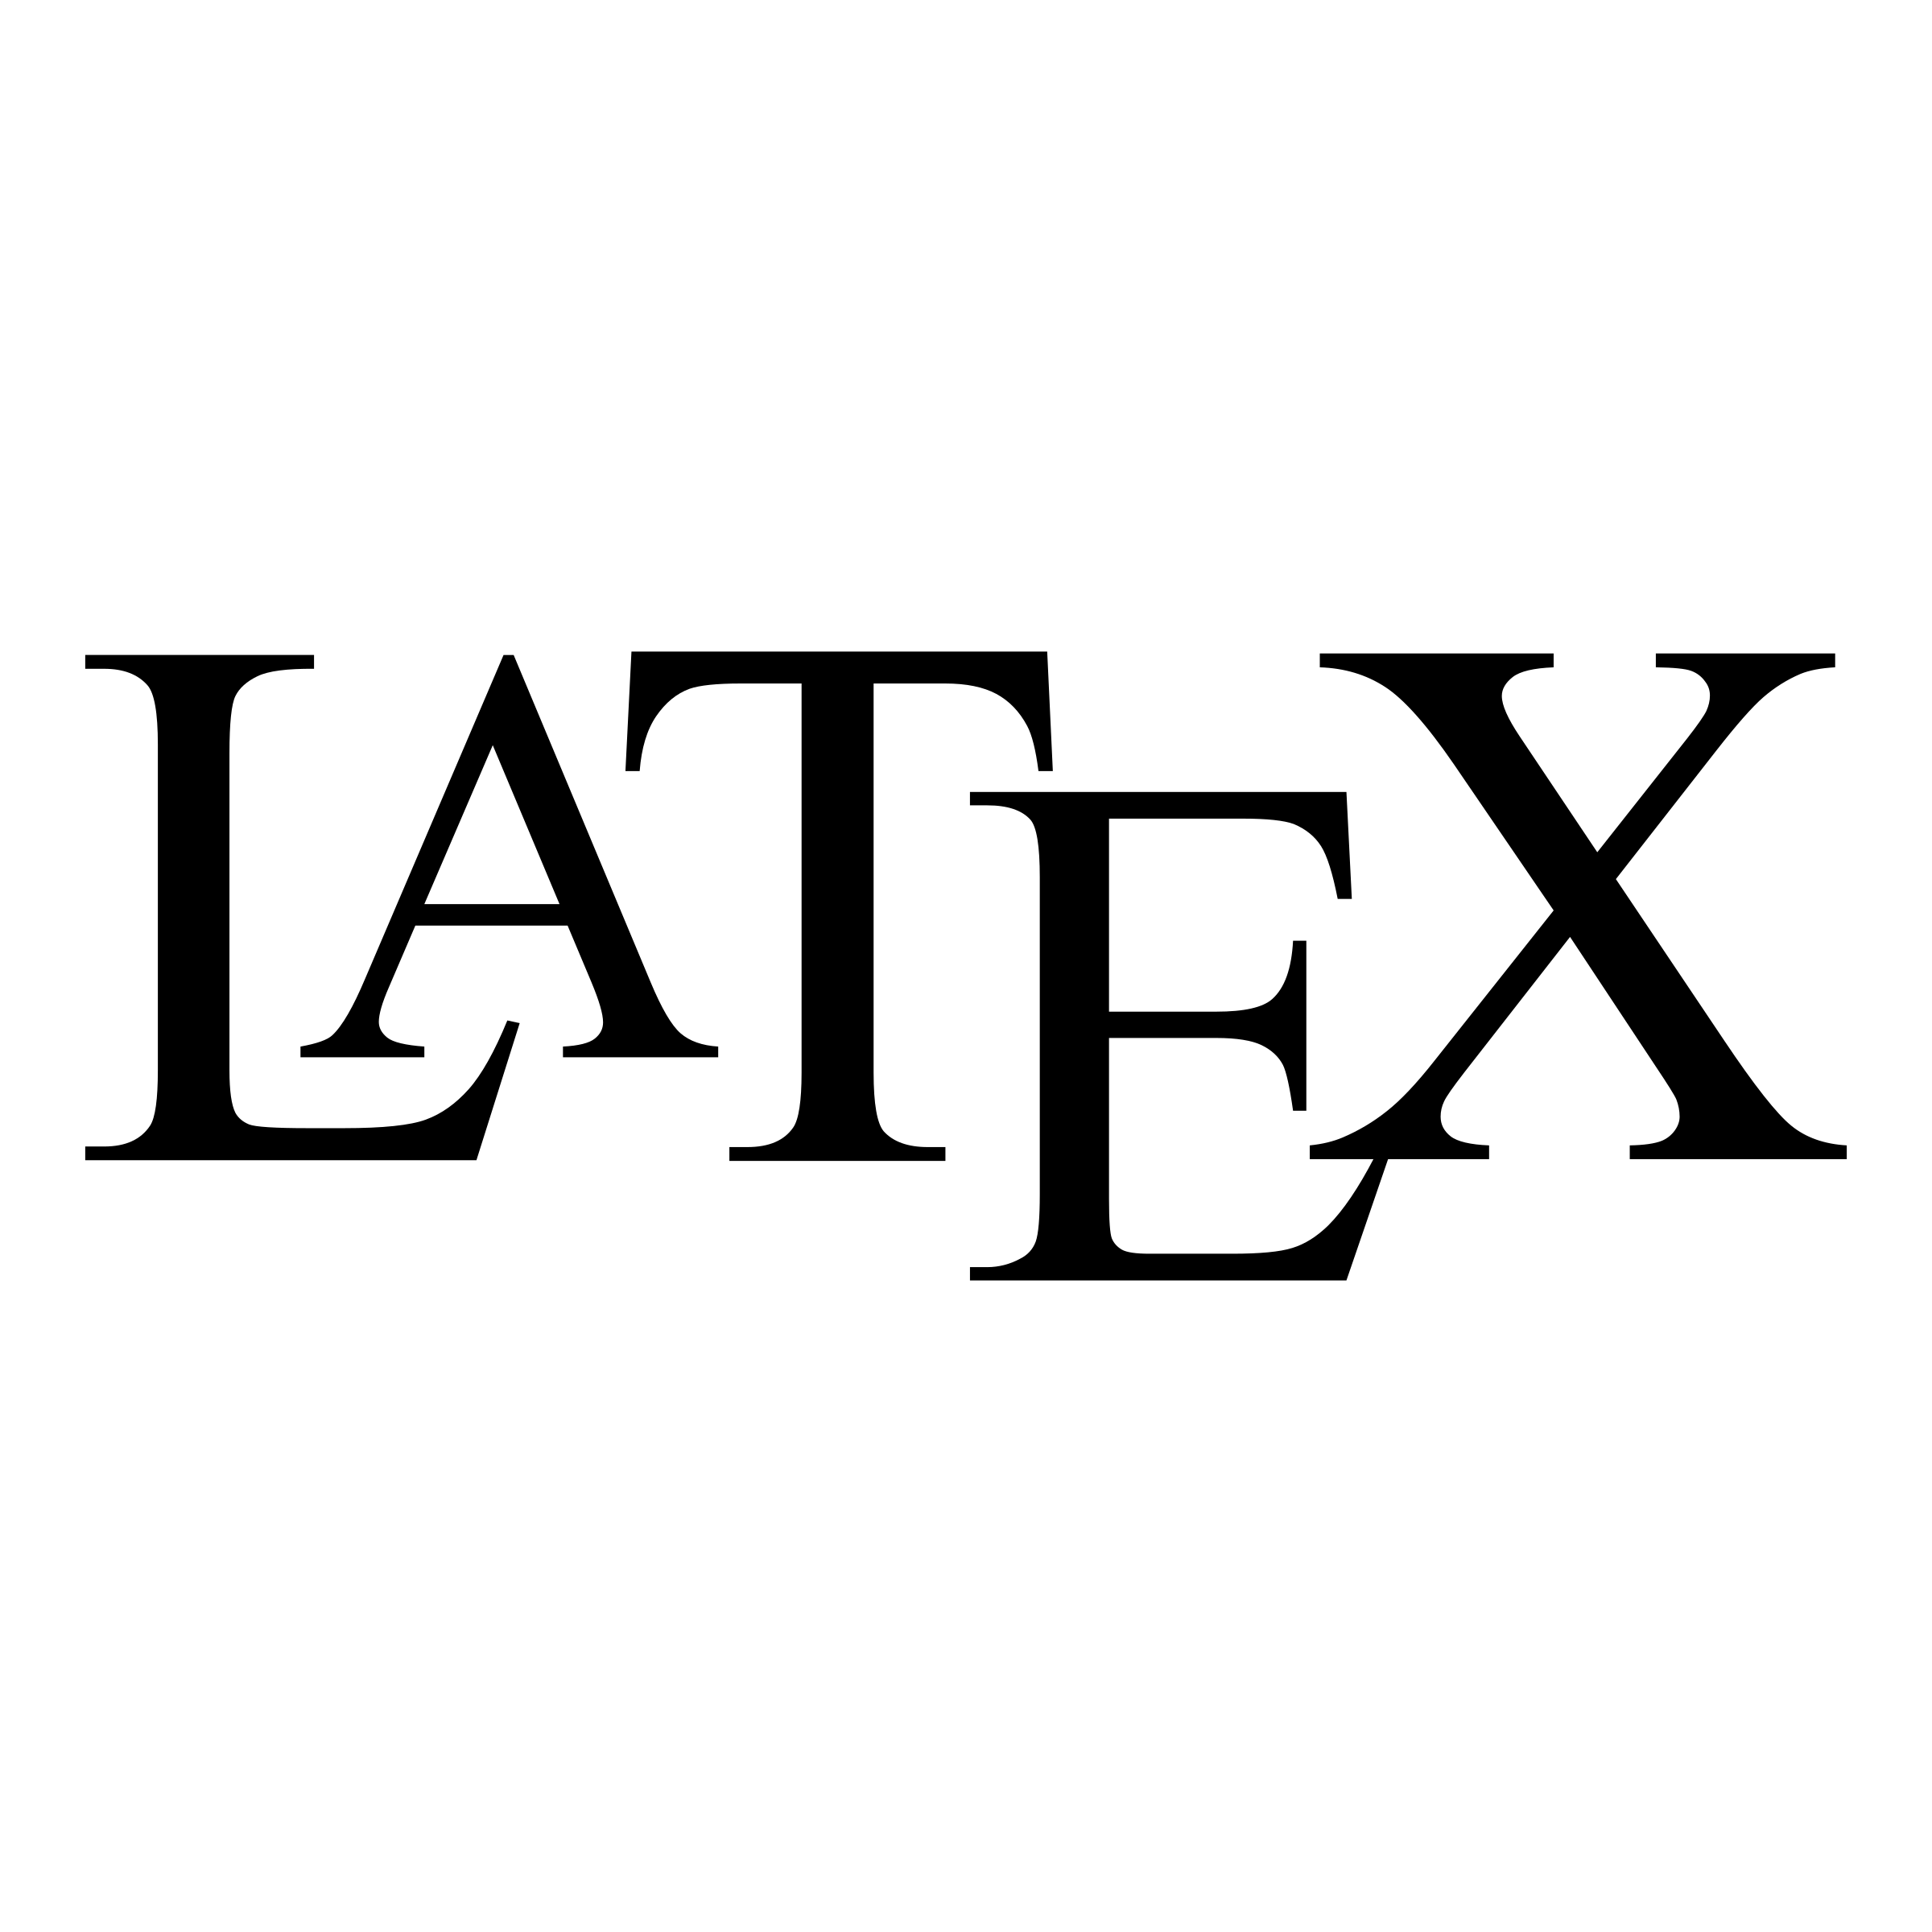
\includegraphics[scale=0.02]{LatexLogo.png}
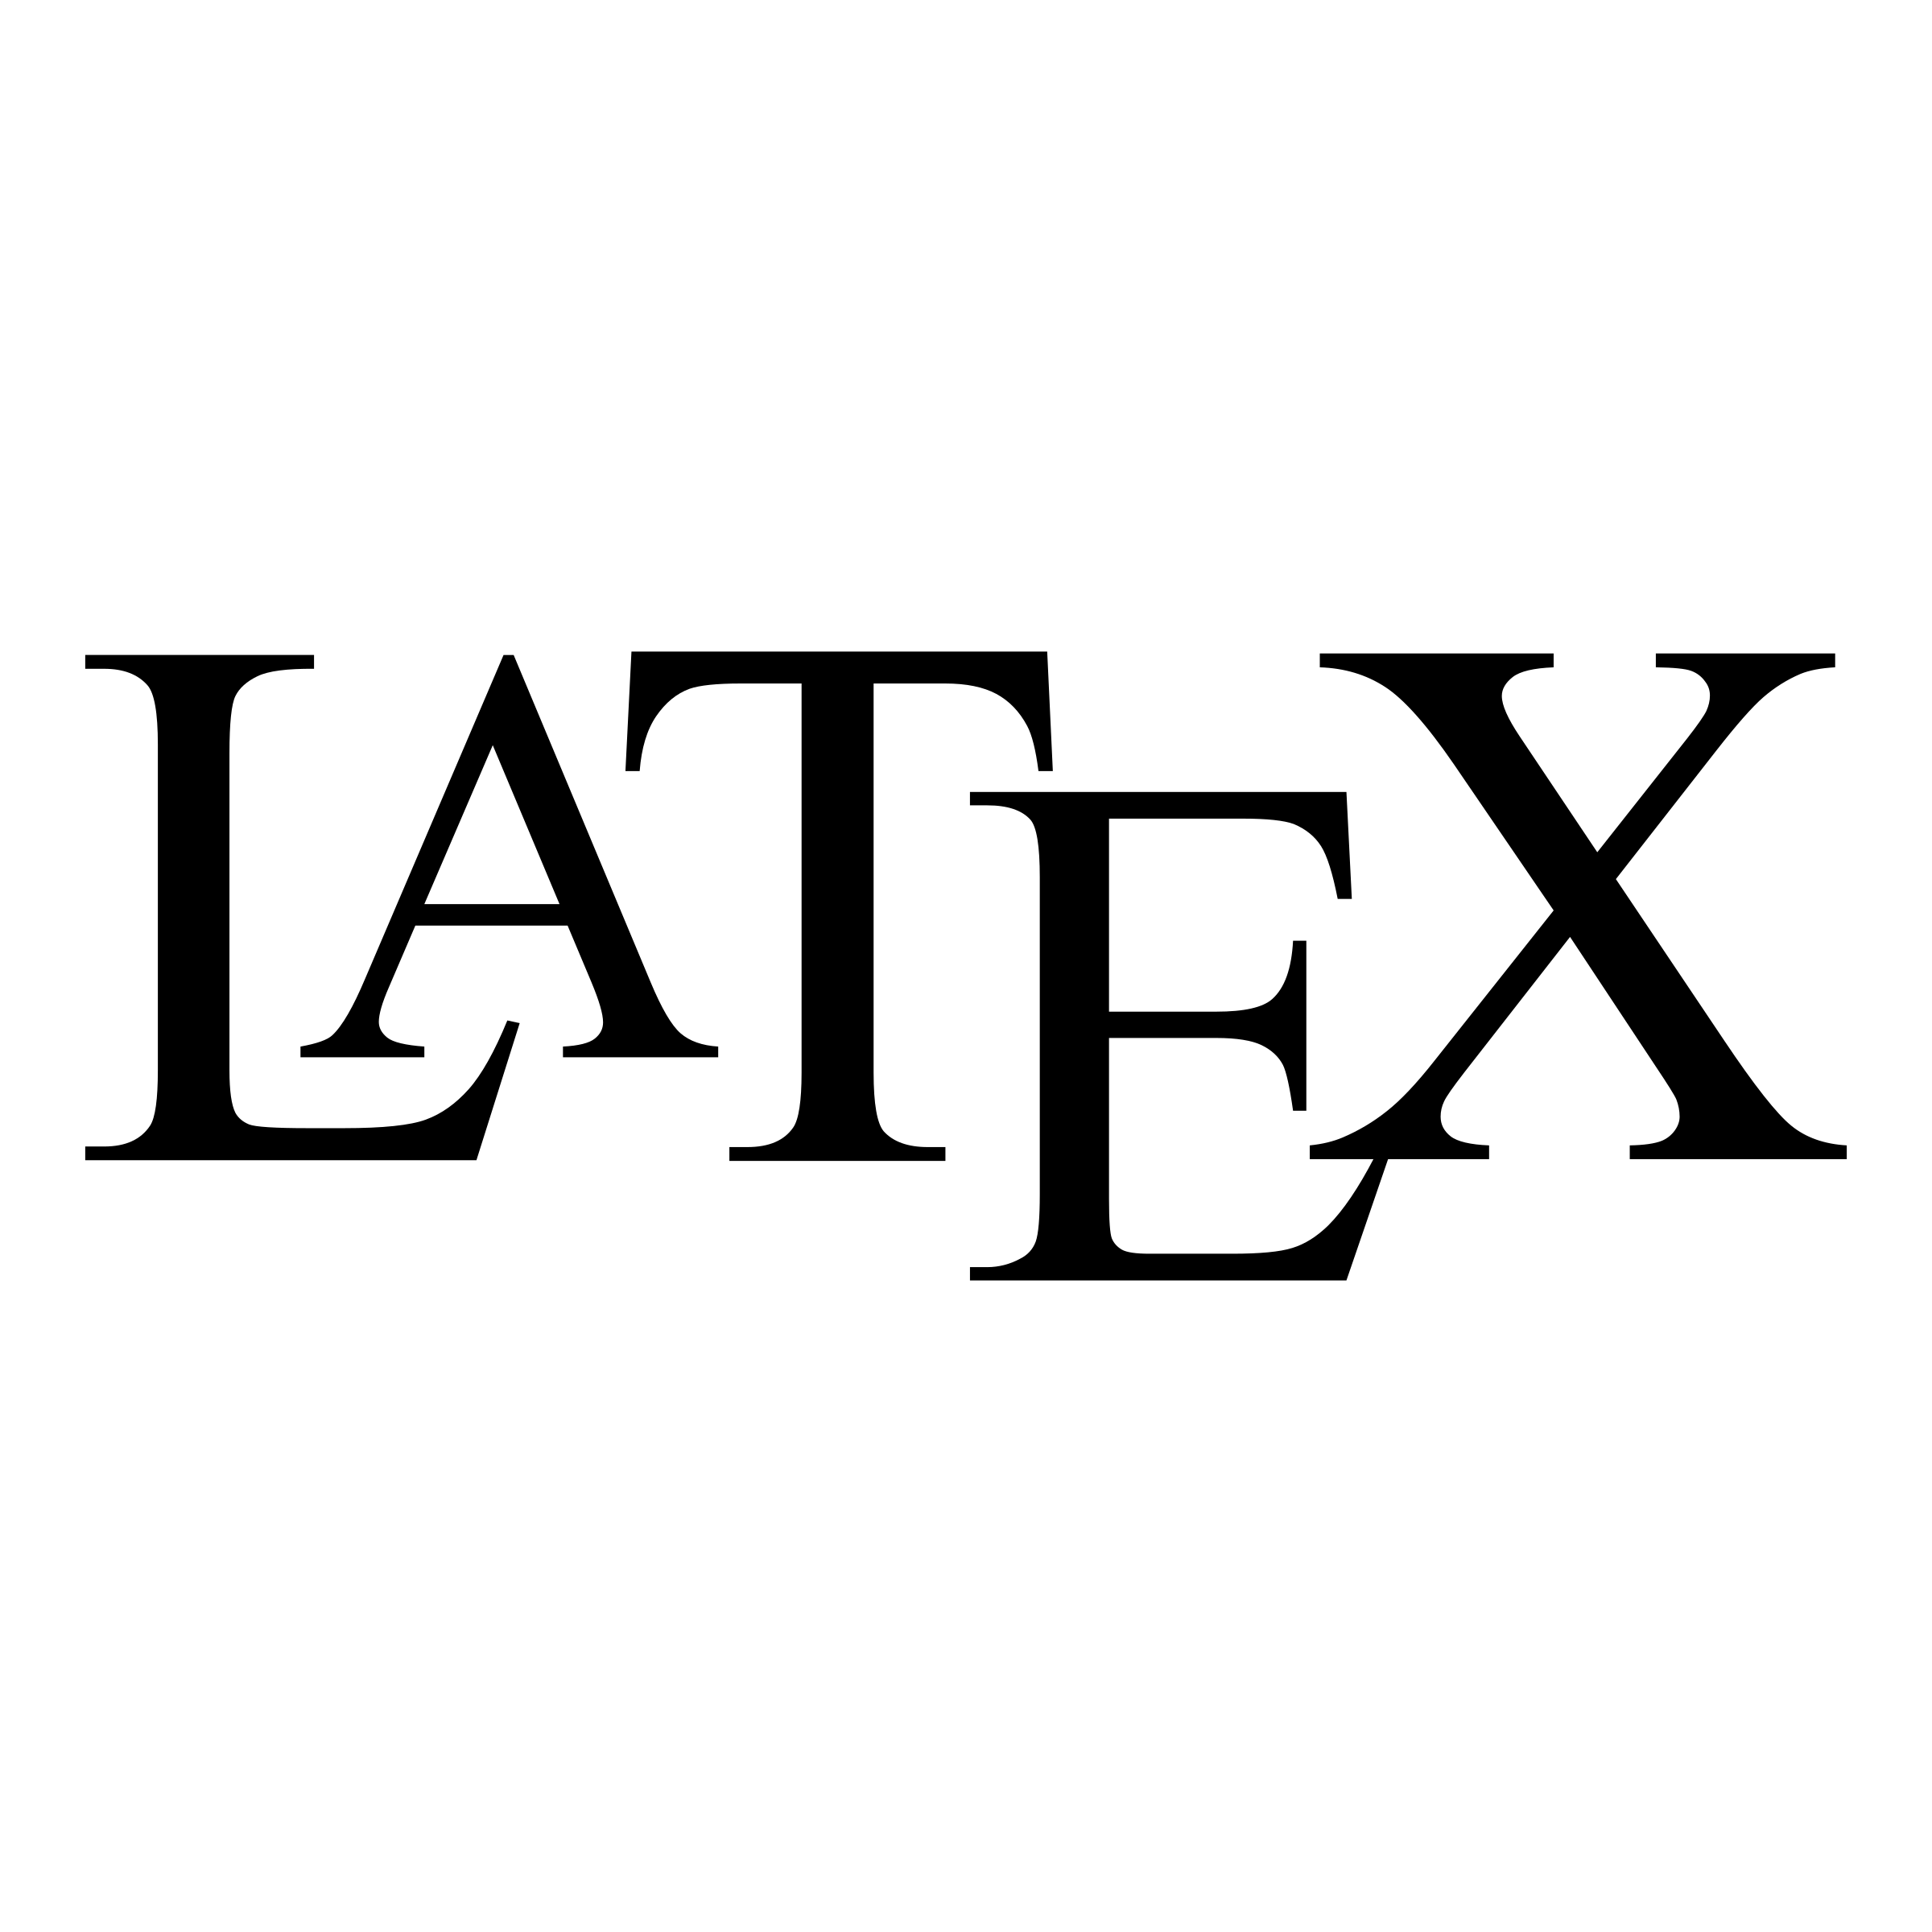
\includegraphics[width=2cm]{LatexLogo.png}
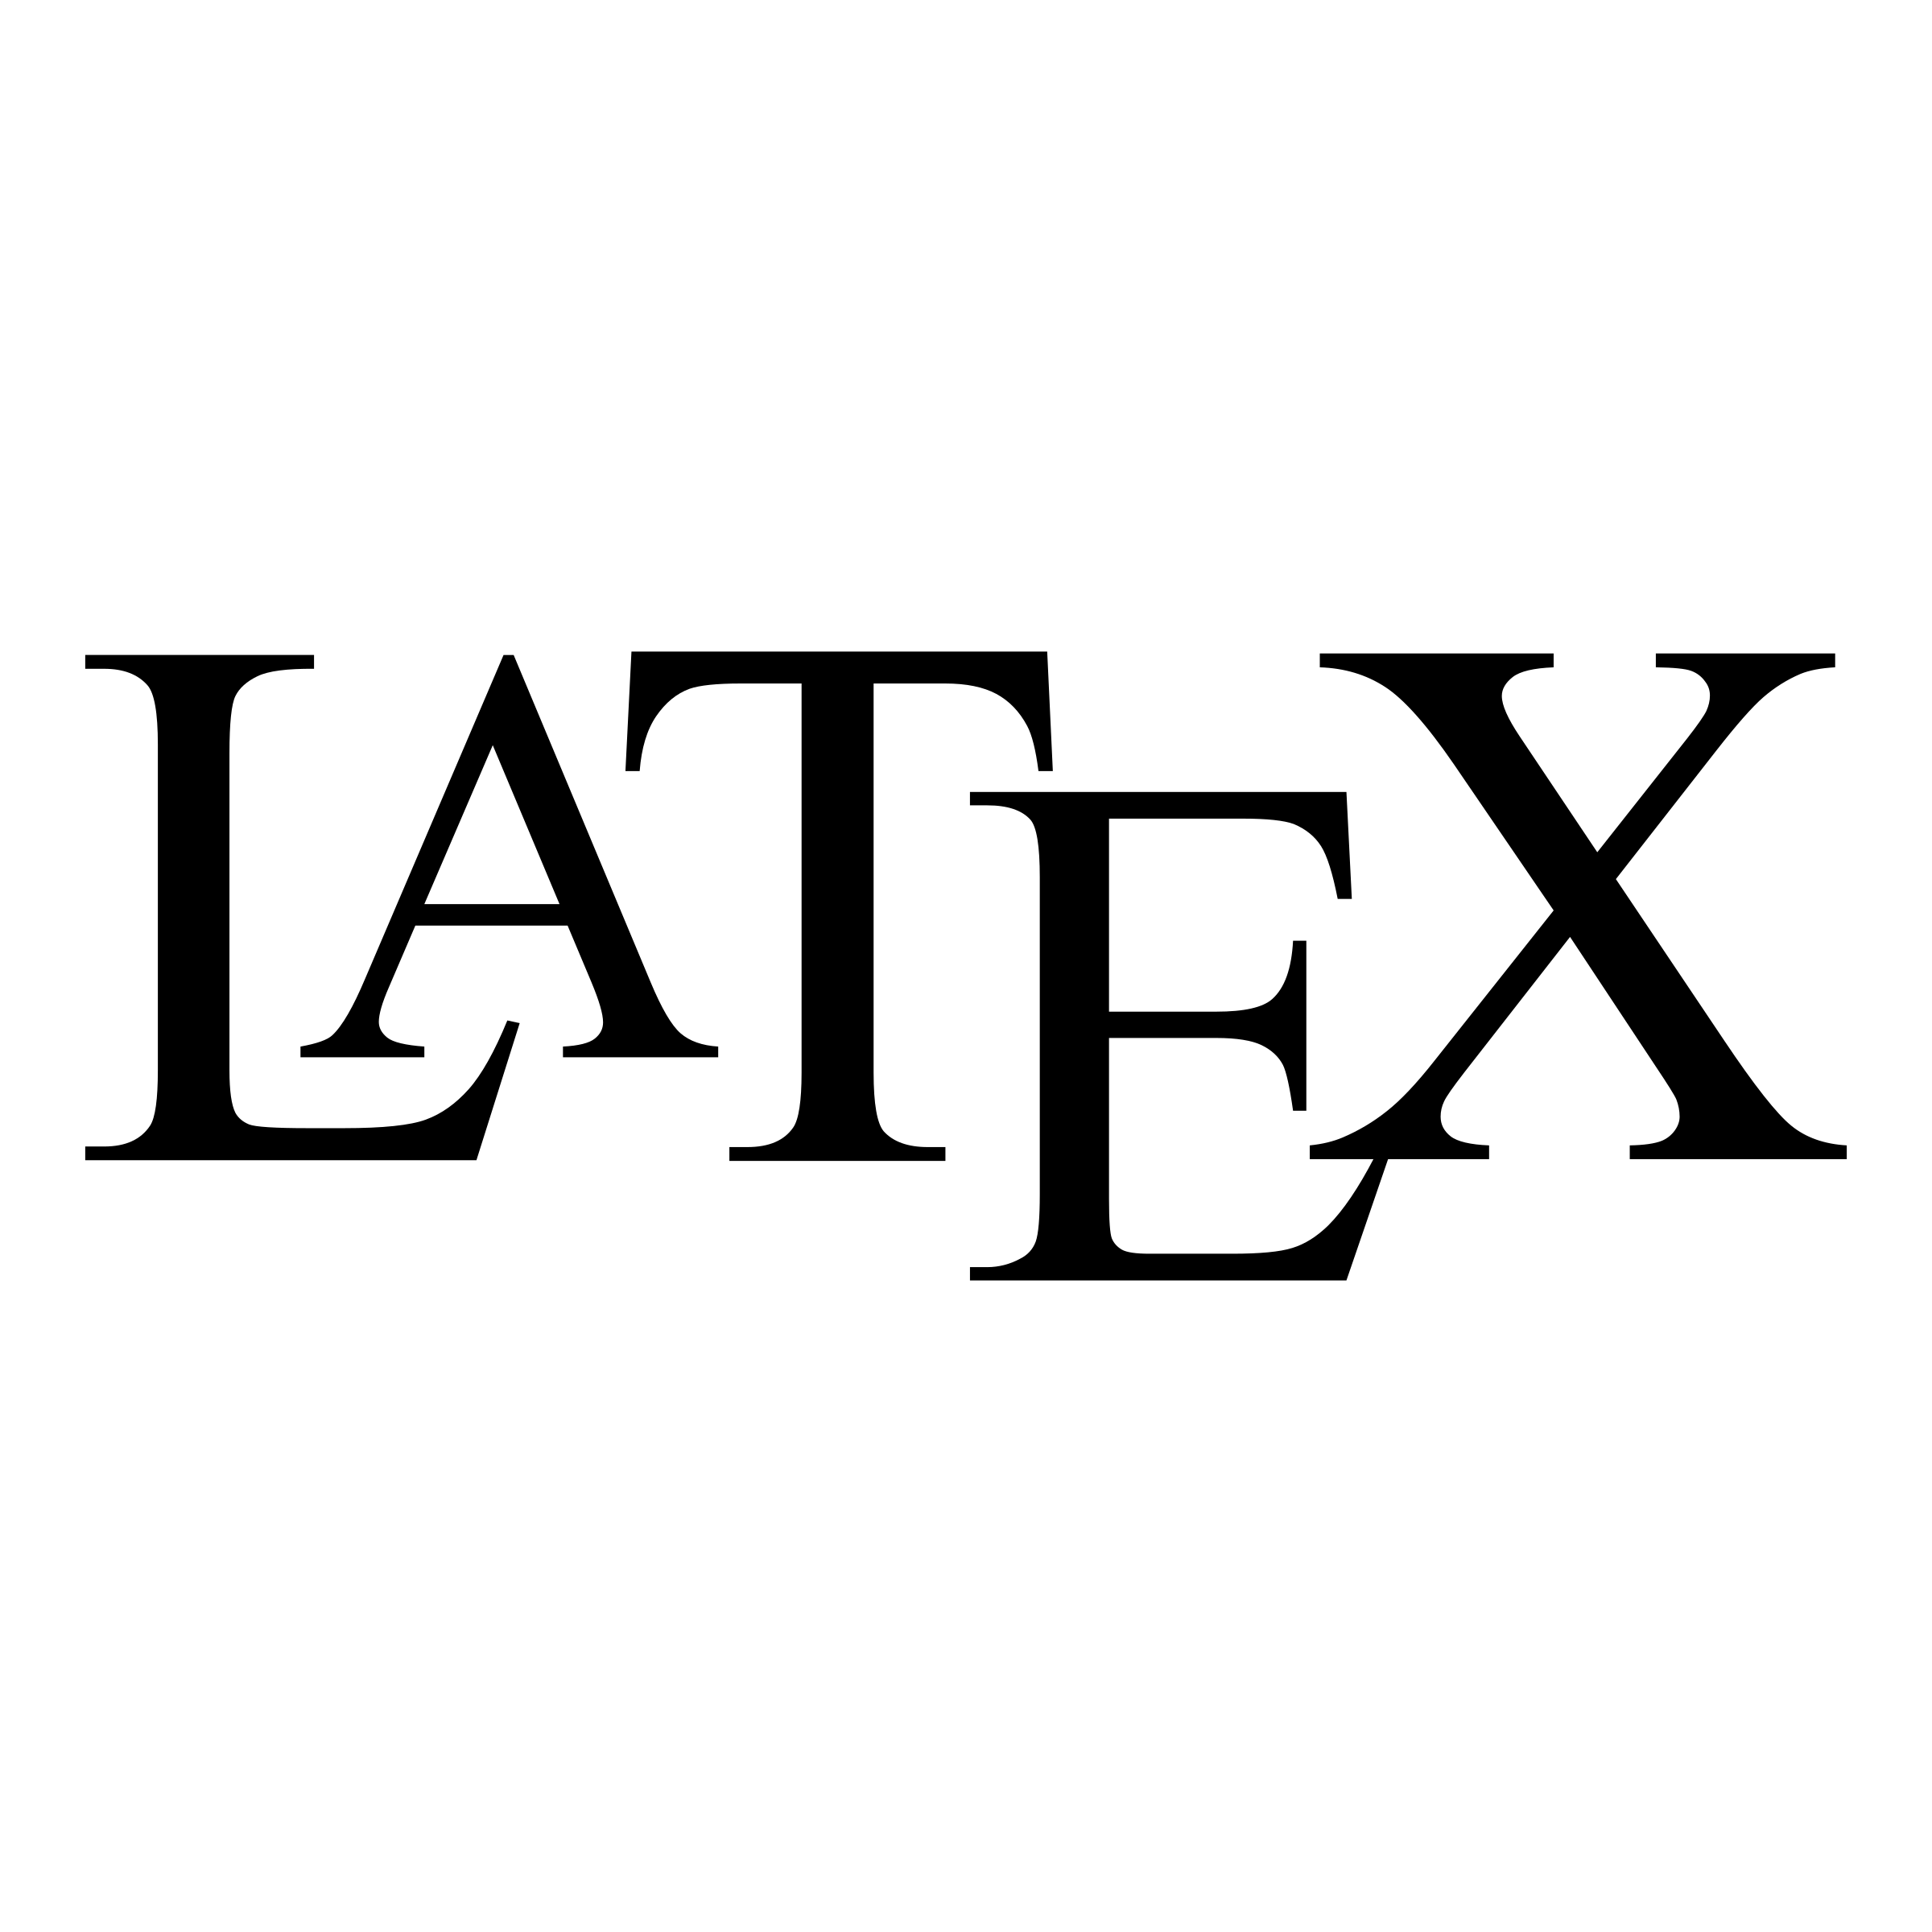
\includegraphics[height=2cm]{LatexLogo.png}
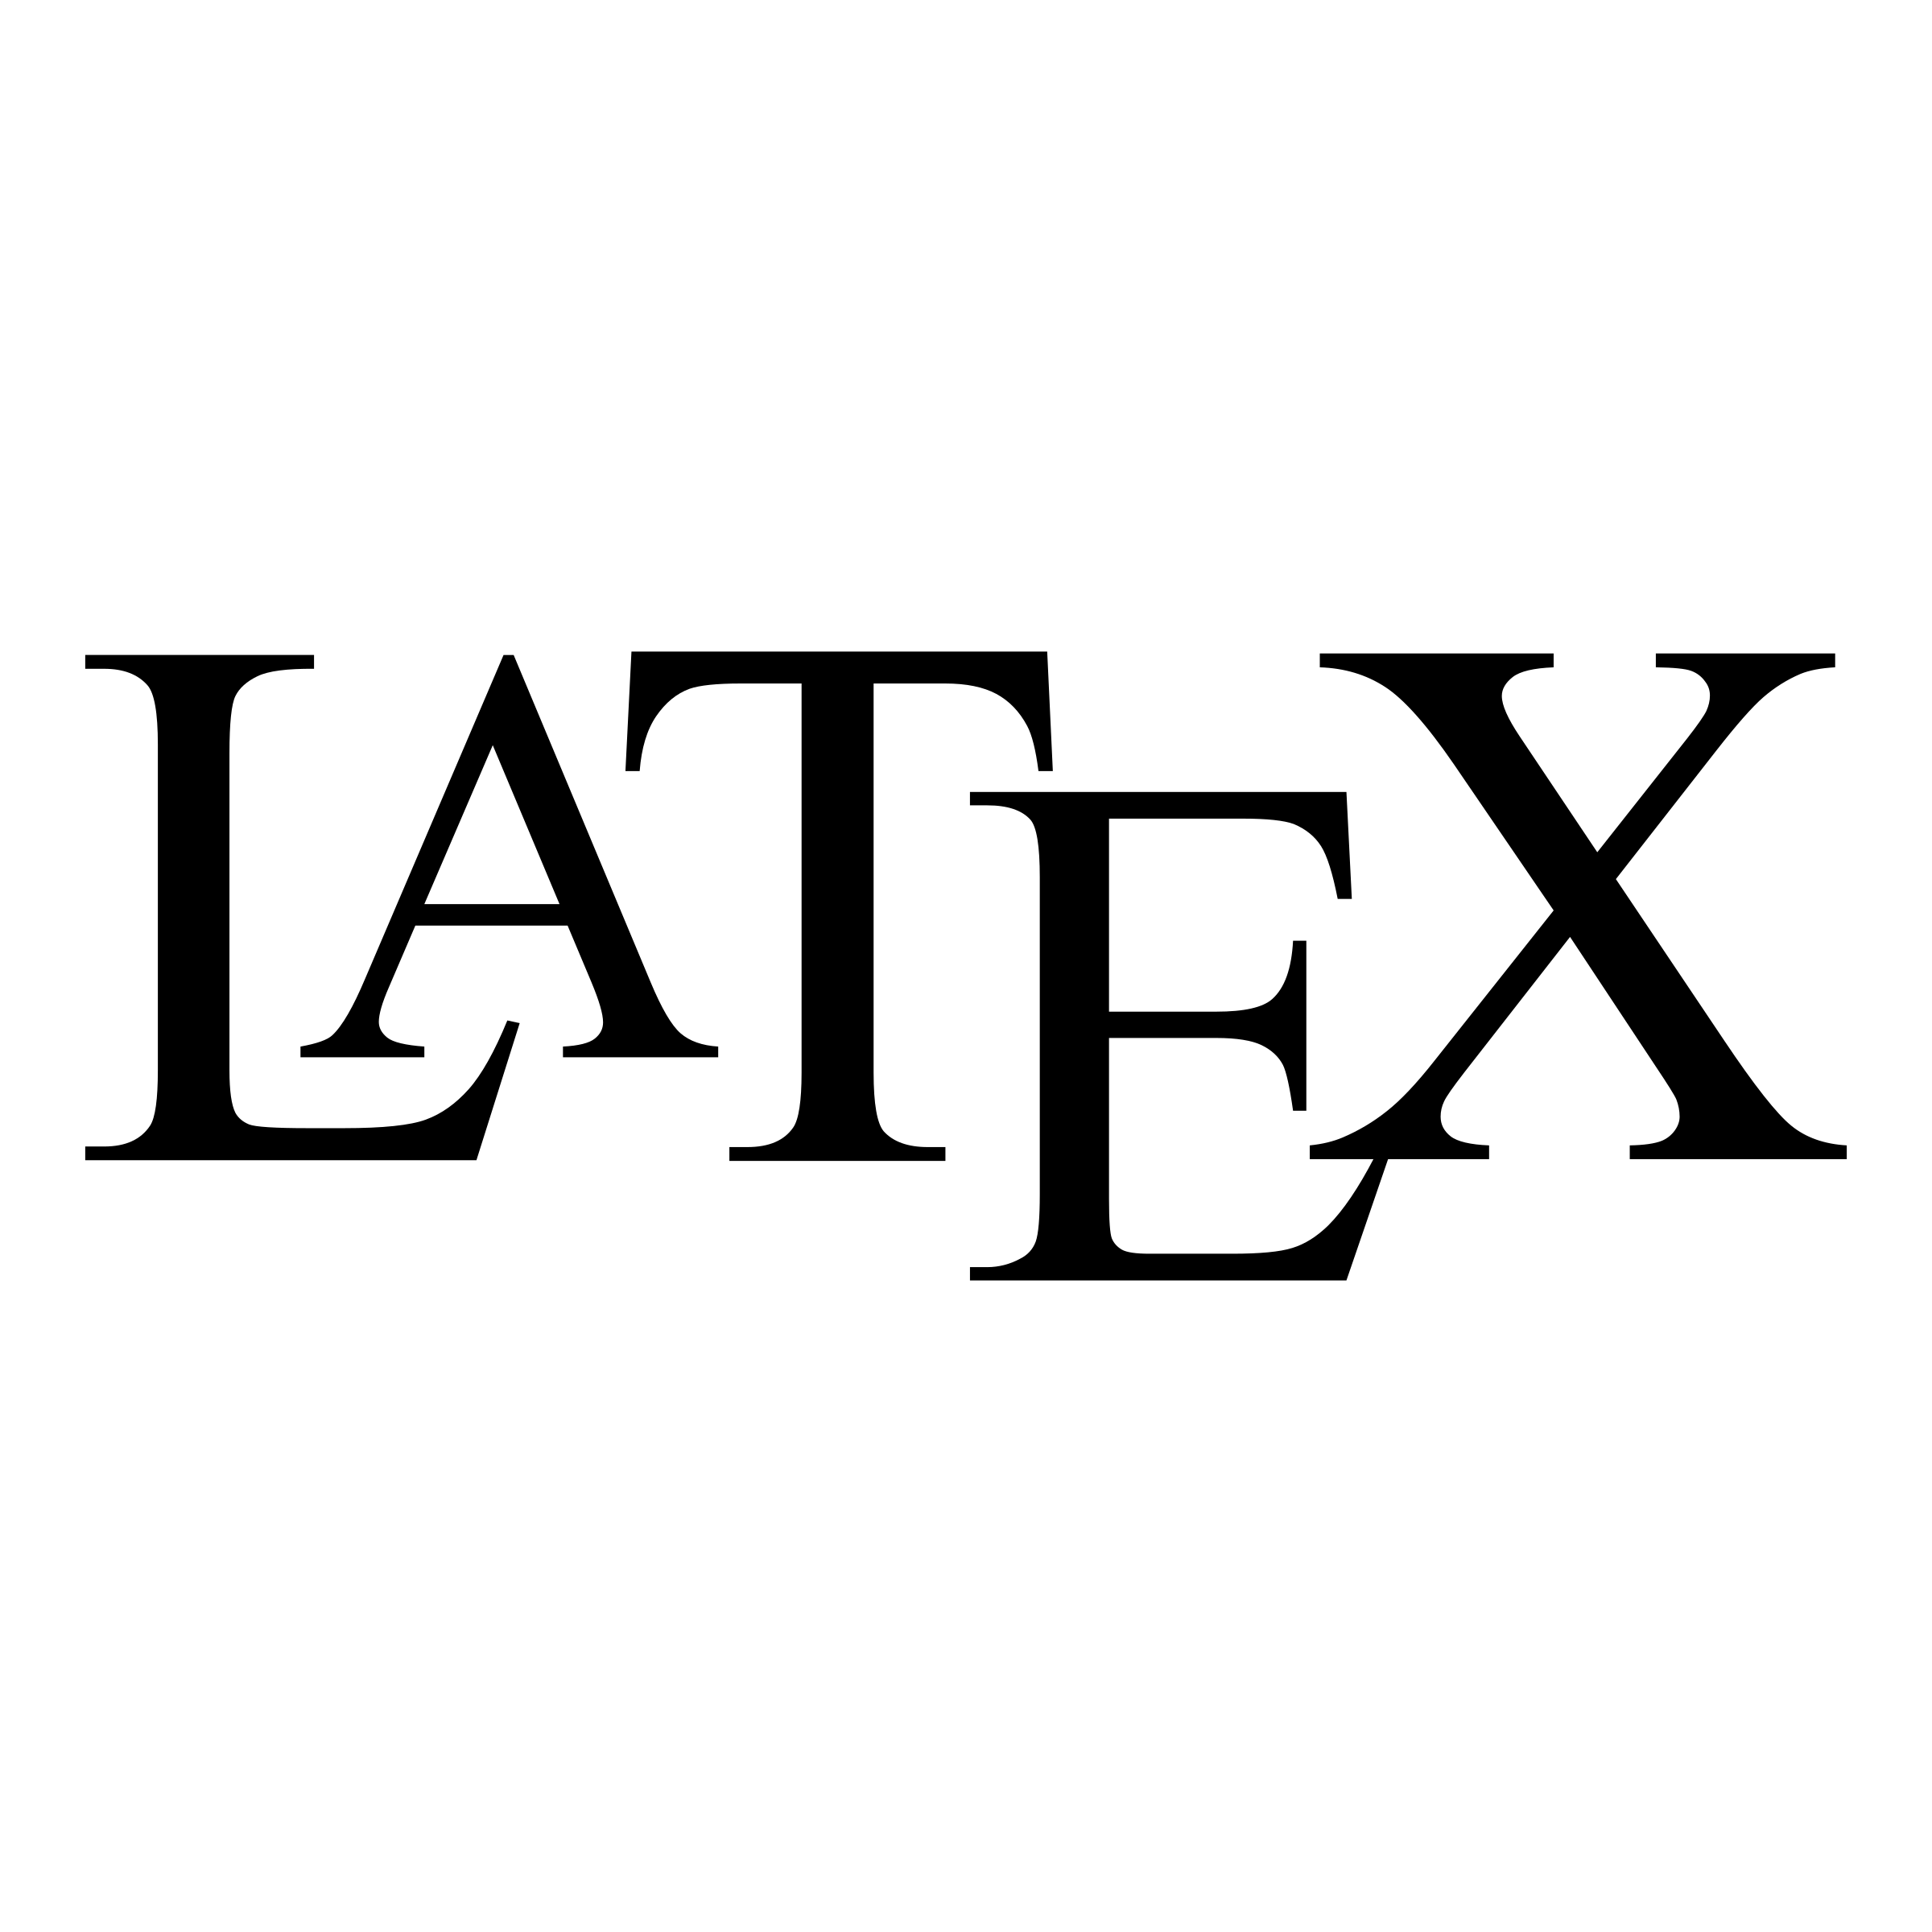
\includegraphics[angle=90, origin=c, scale=0.02]{LatexLogo.png}
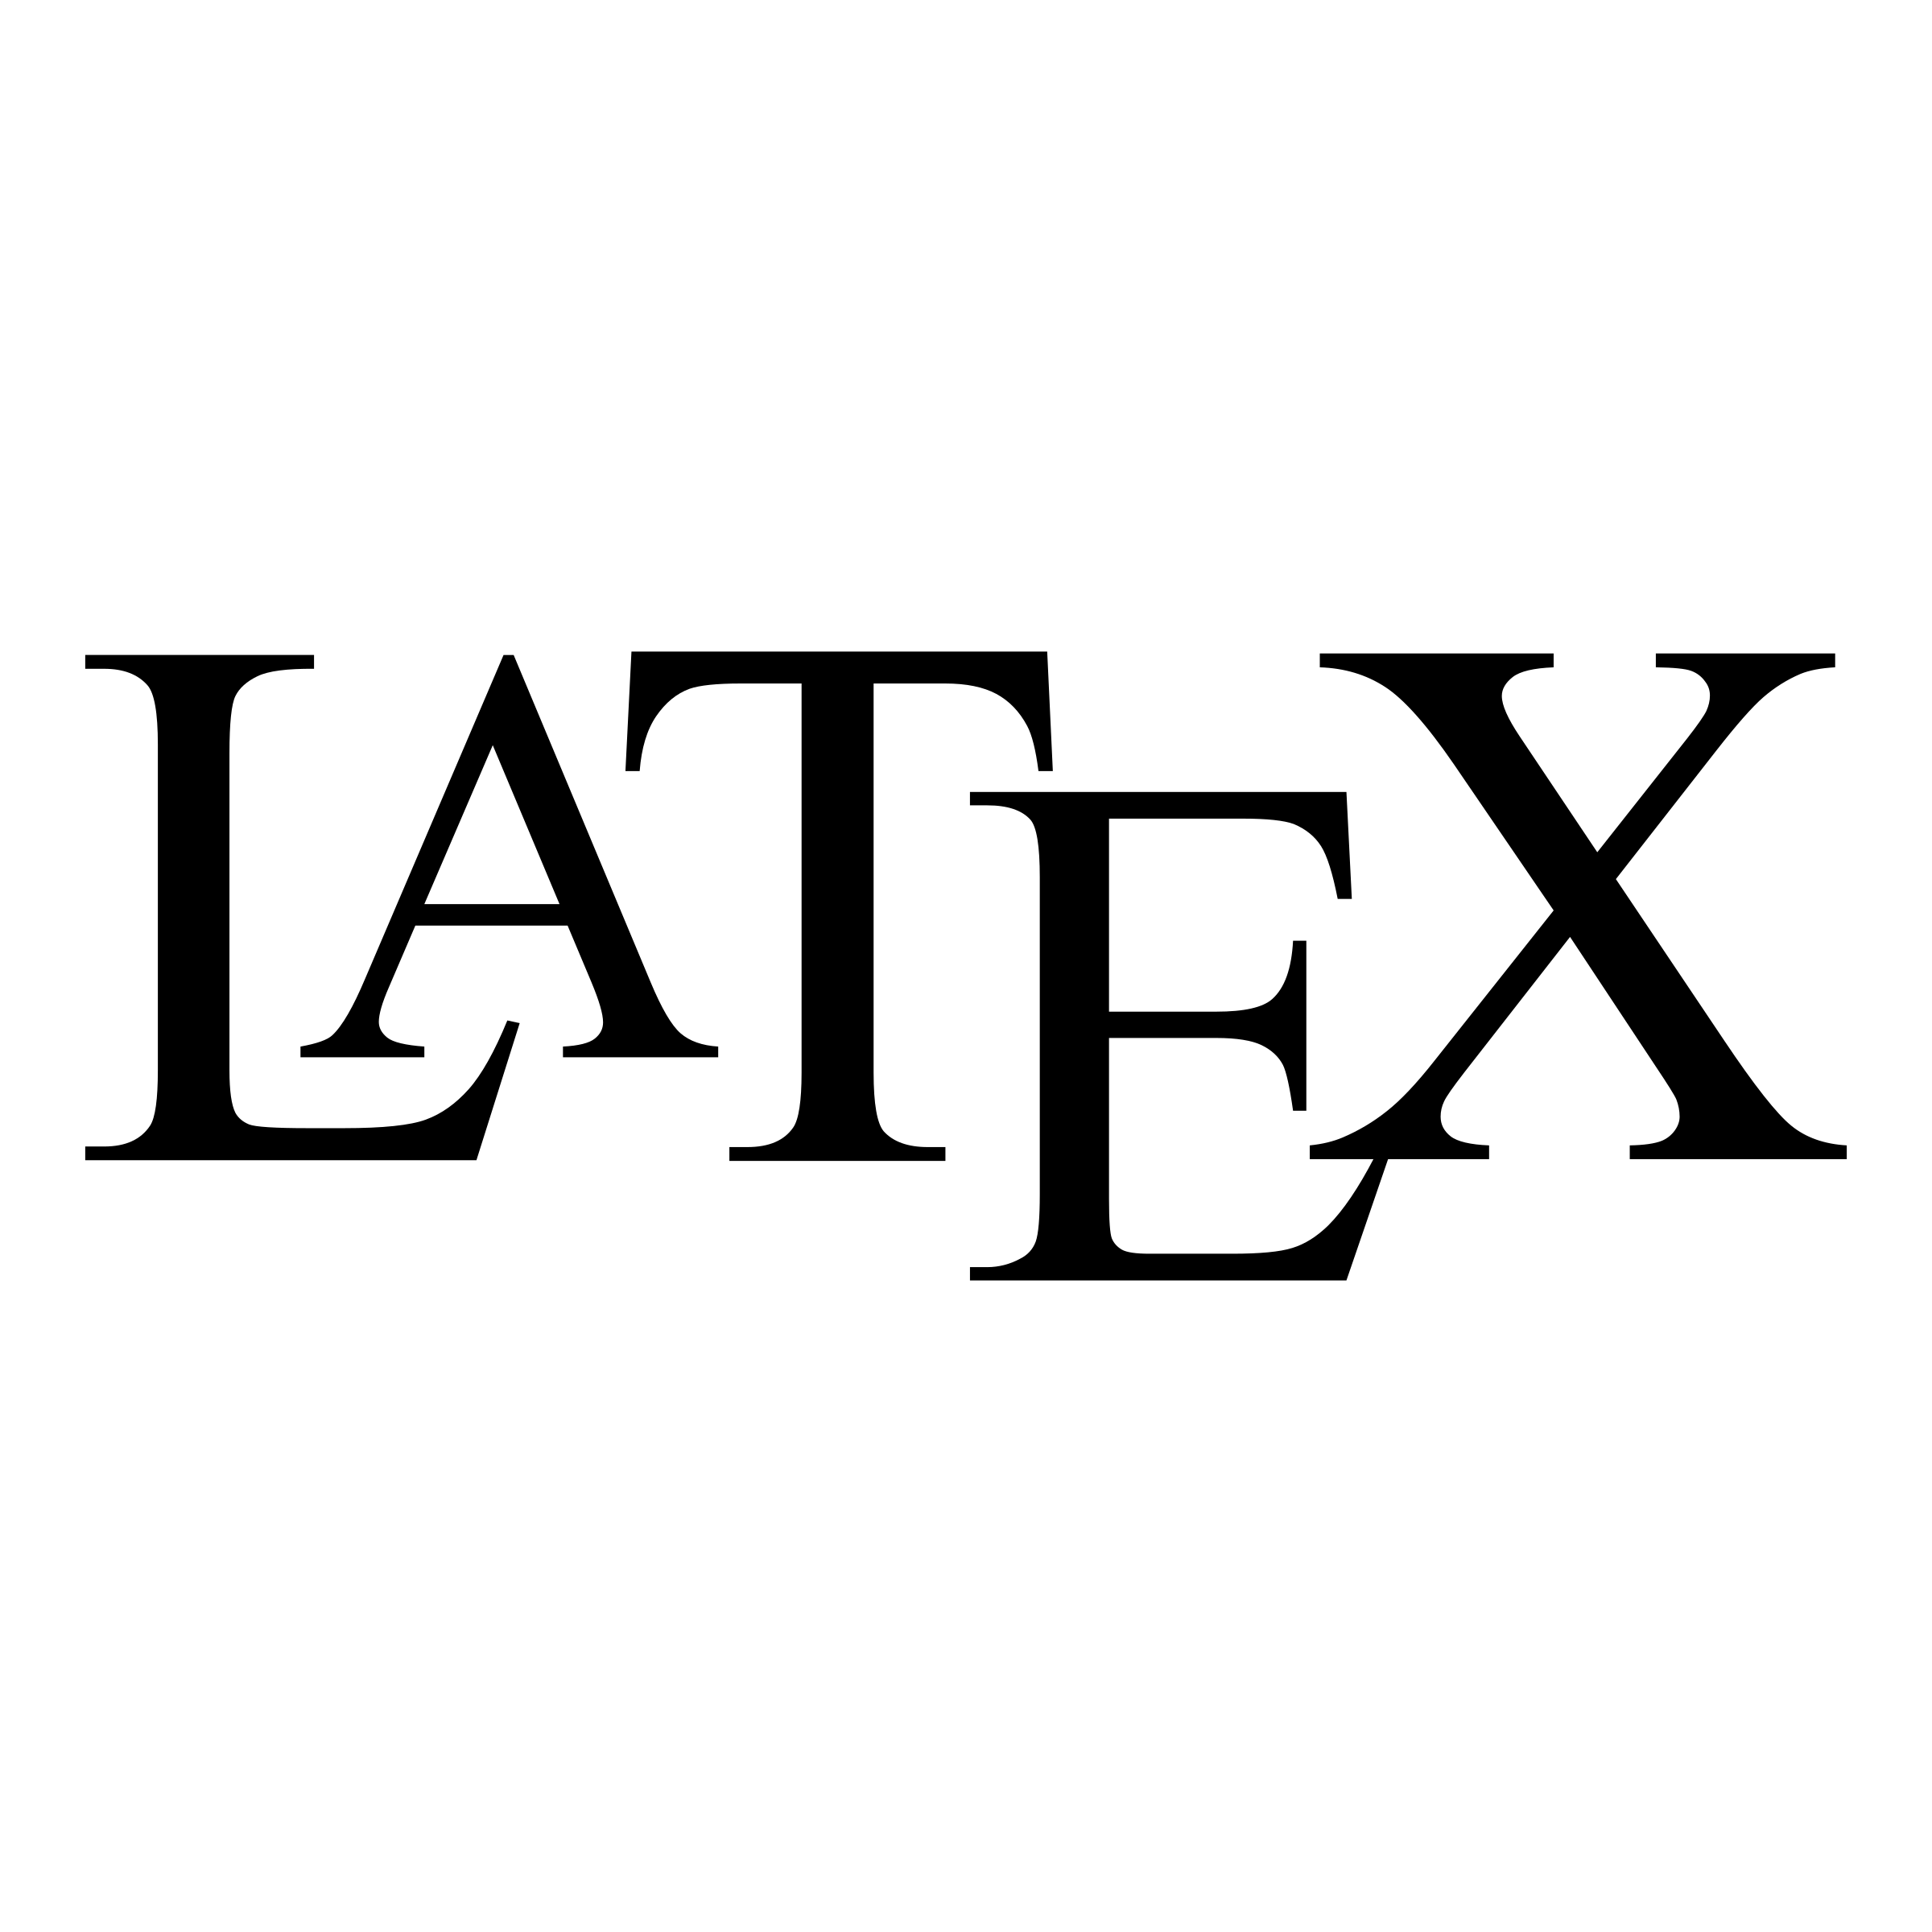
\includegraphics[draft, scale=0.02]{LatexLogo.png}

\subsection{Float Figure}
\subsubsection{Overview}
\begin{figure}[!htbp]
    \centering
    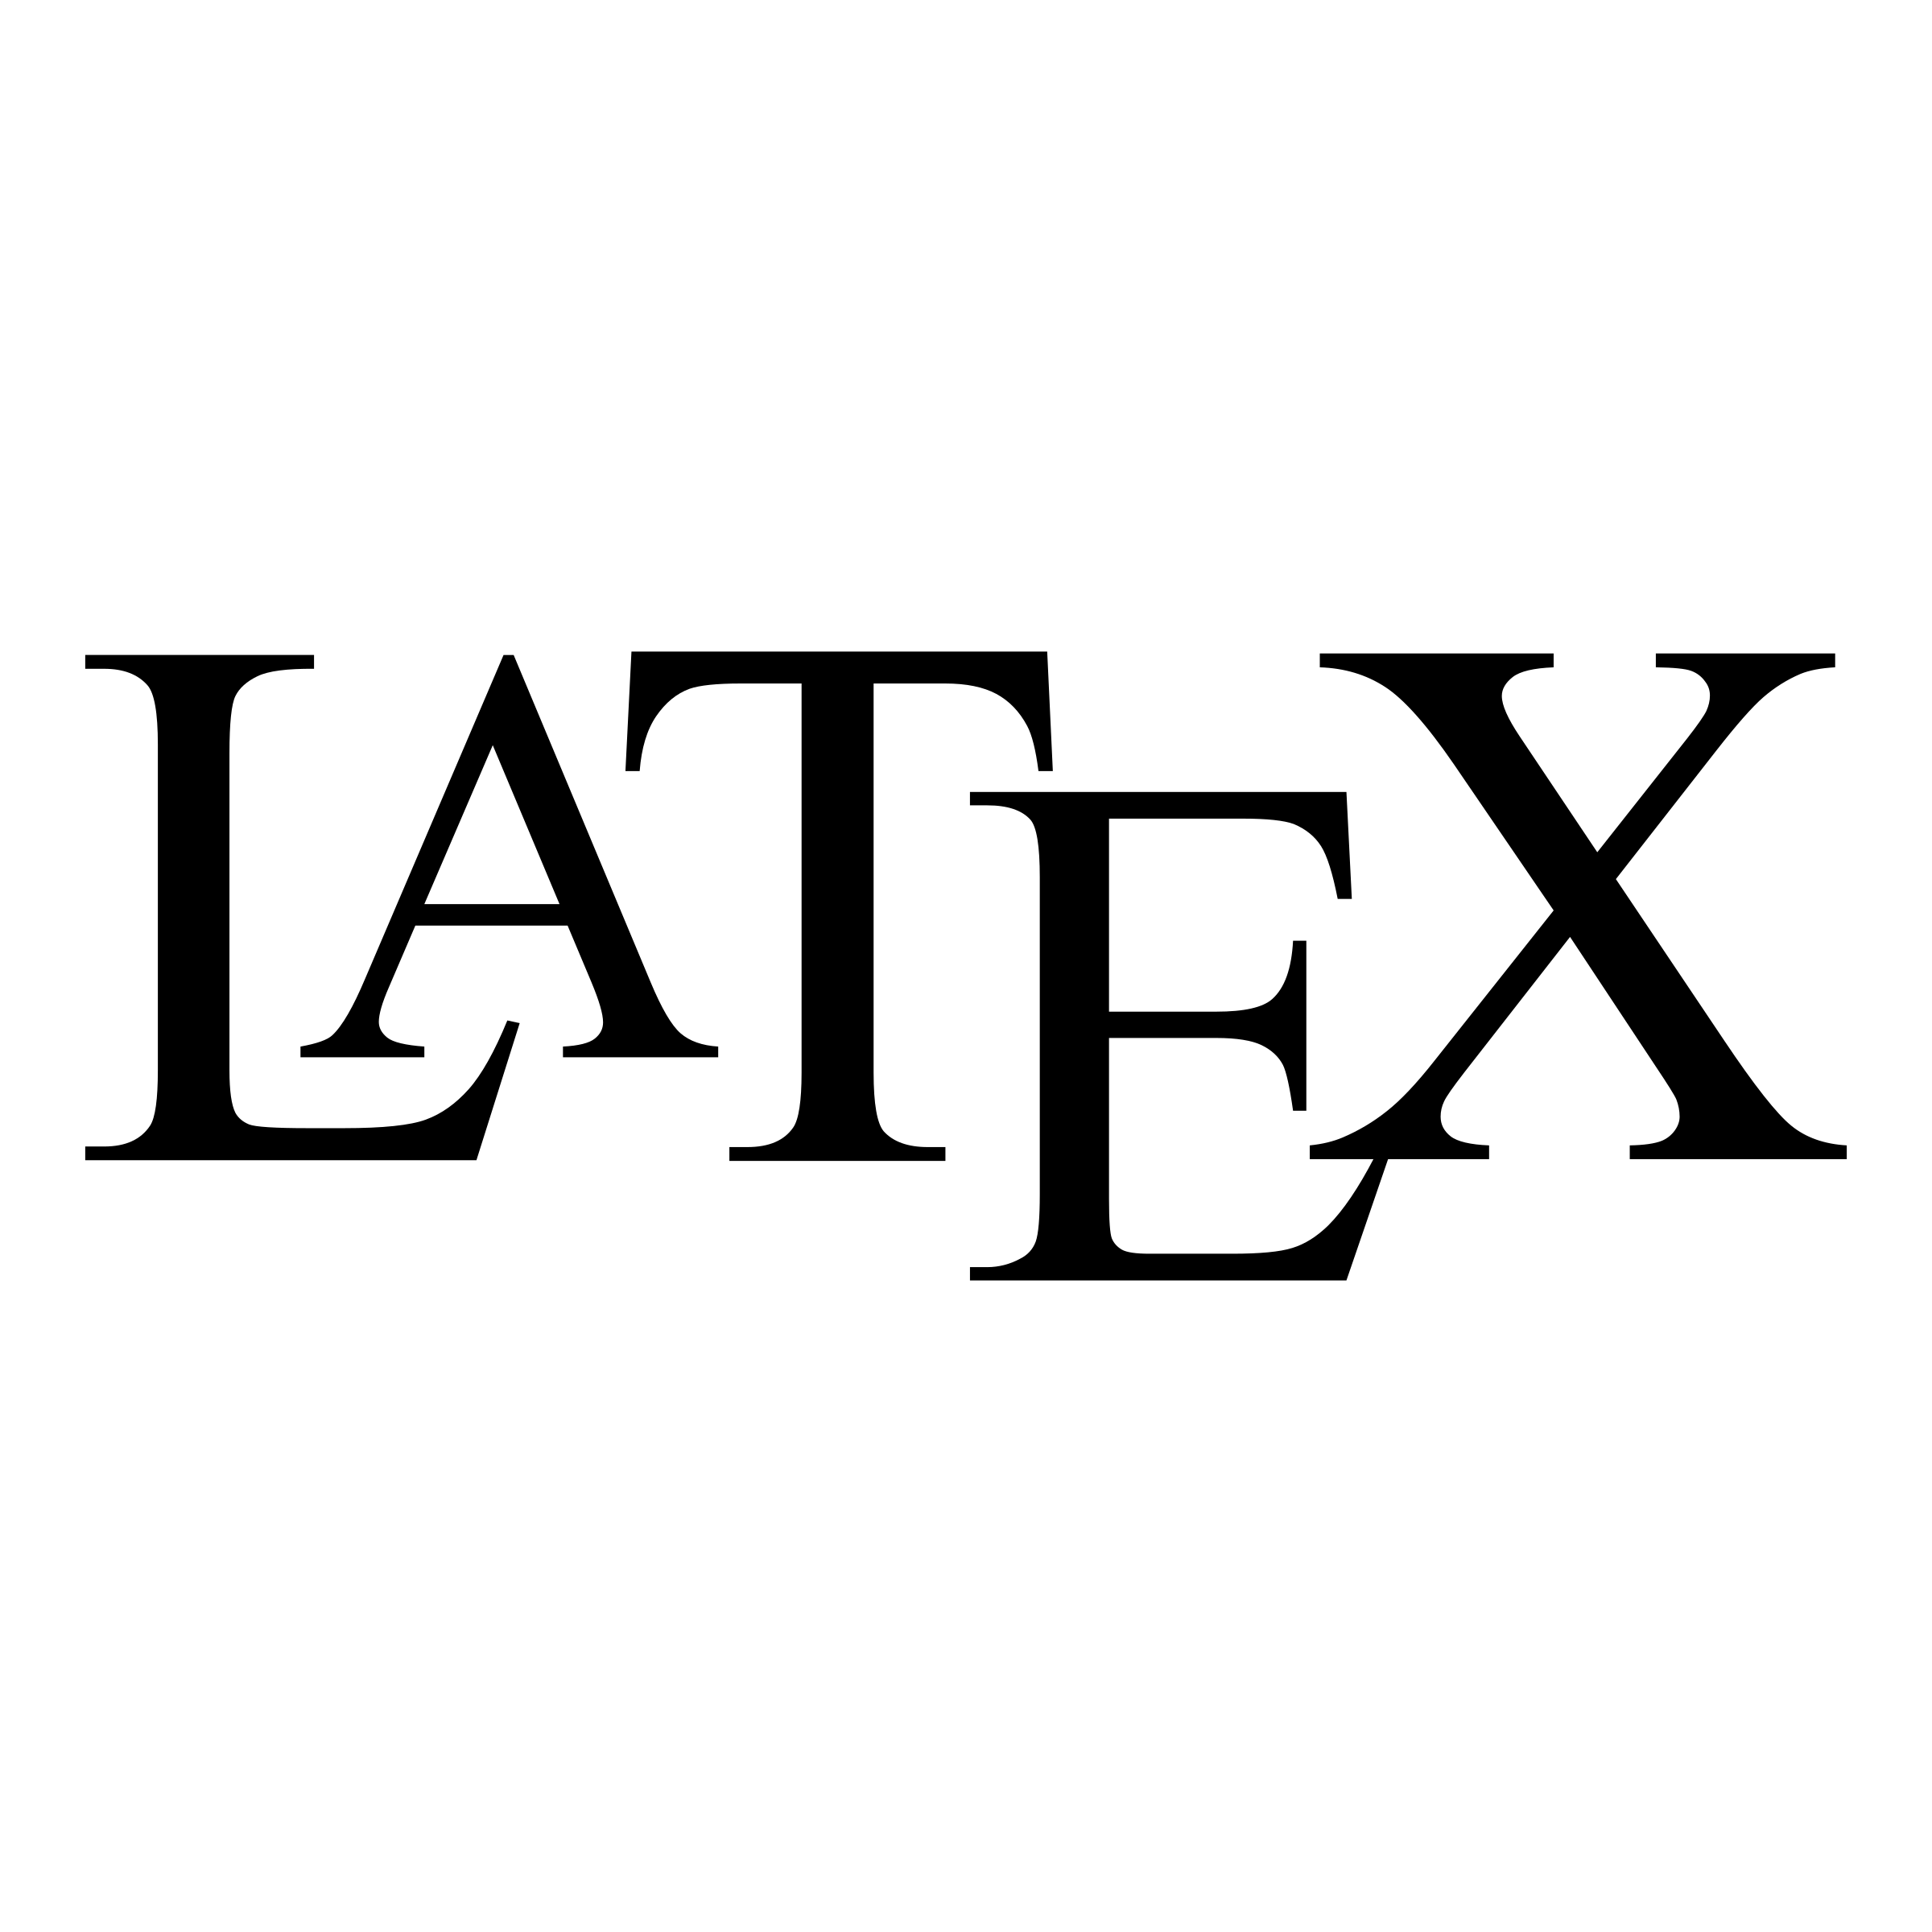
\includegraphics[scale=0.05]{LatexLogo.png}
    \bicaption[Latex Logo]{\label{fig-float} Latex Logo - Example Of Float Figure}[标志]{浮动图片的例子}
\end{figure}

\subsubsection{Rotated Figure}
% must usepackage rotfloat
\begin{sidewaysfigure}
    \centering
    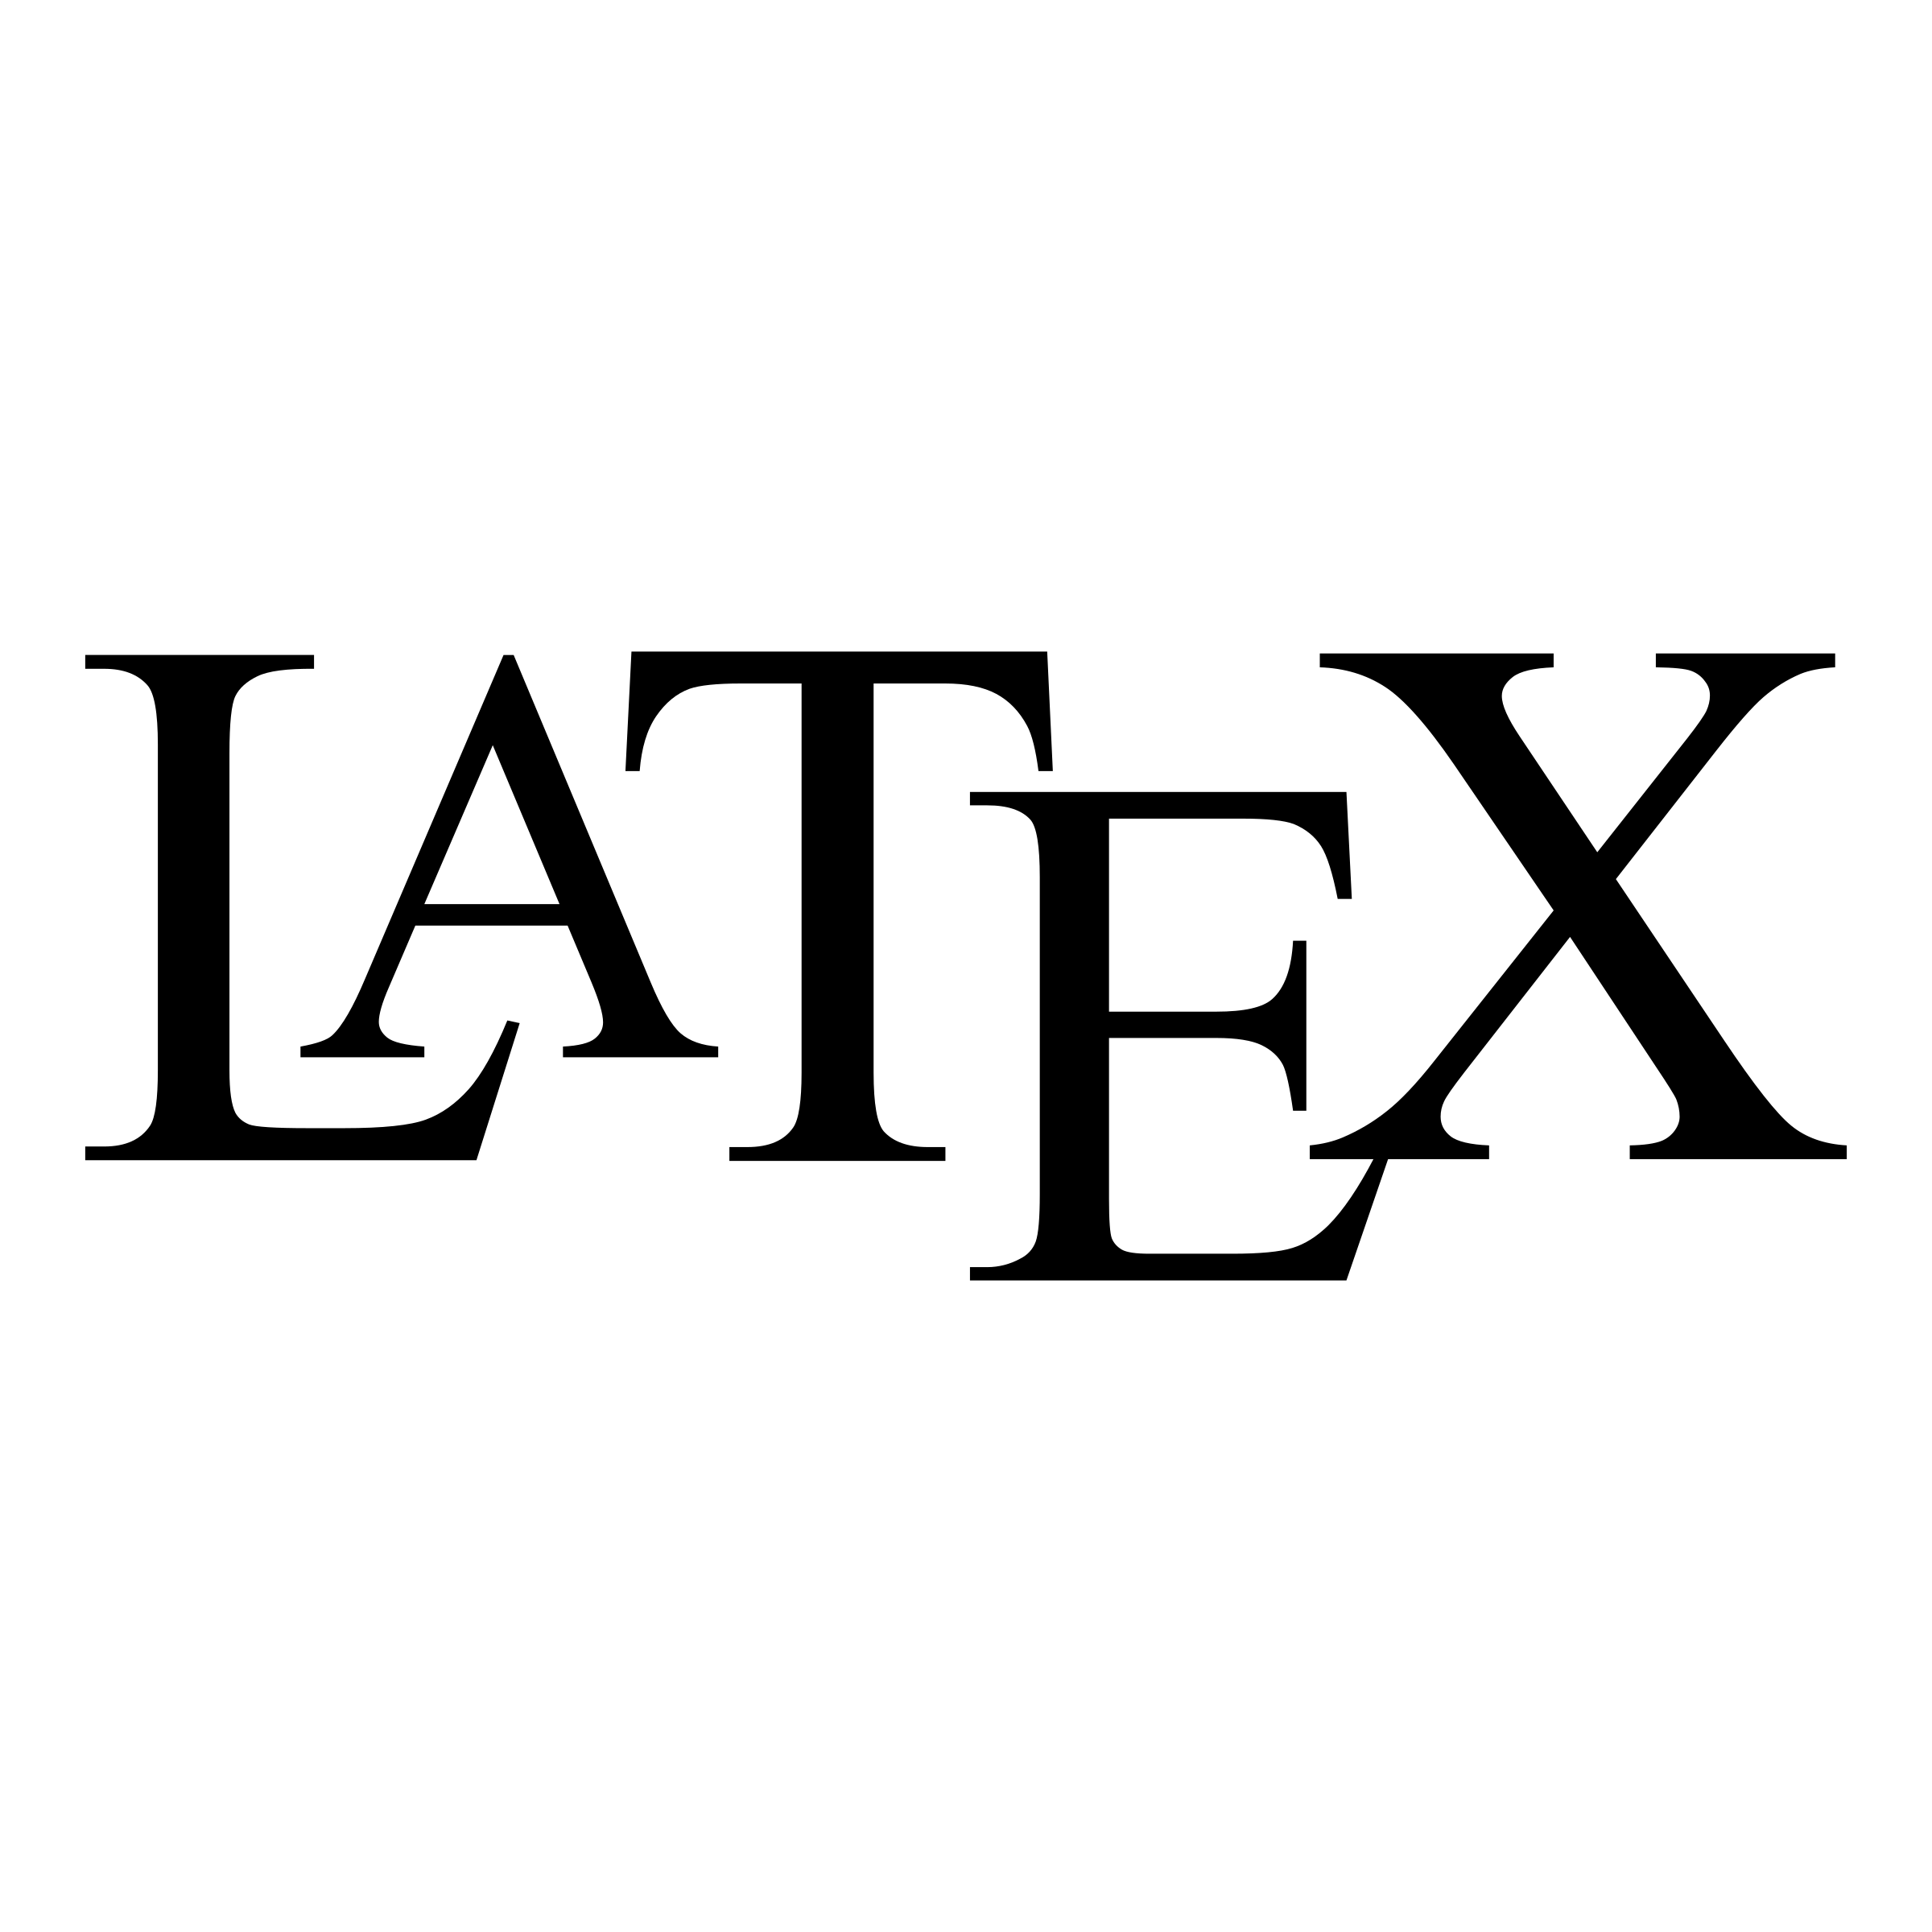
\includegraphics[scale=0.1]{LatexLogo.png}
    \caption{Latex Logo}
\end{sidewaysfigure}

\subsubsection{Side By Side}
\paragraph{Figure With Words}
\begin{figure}[H]
    \centering
    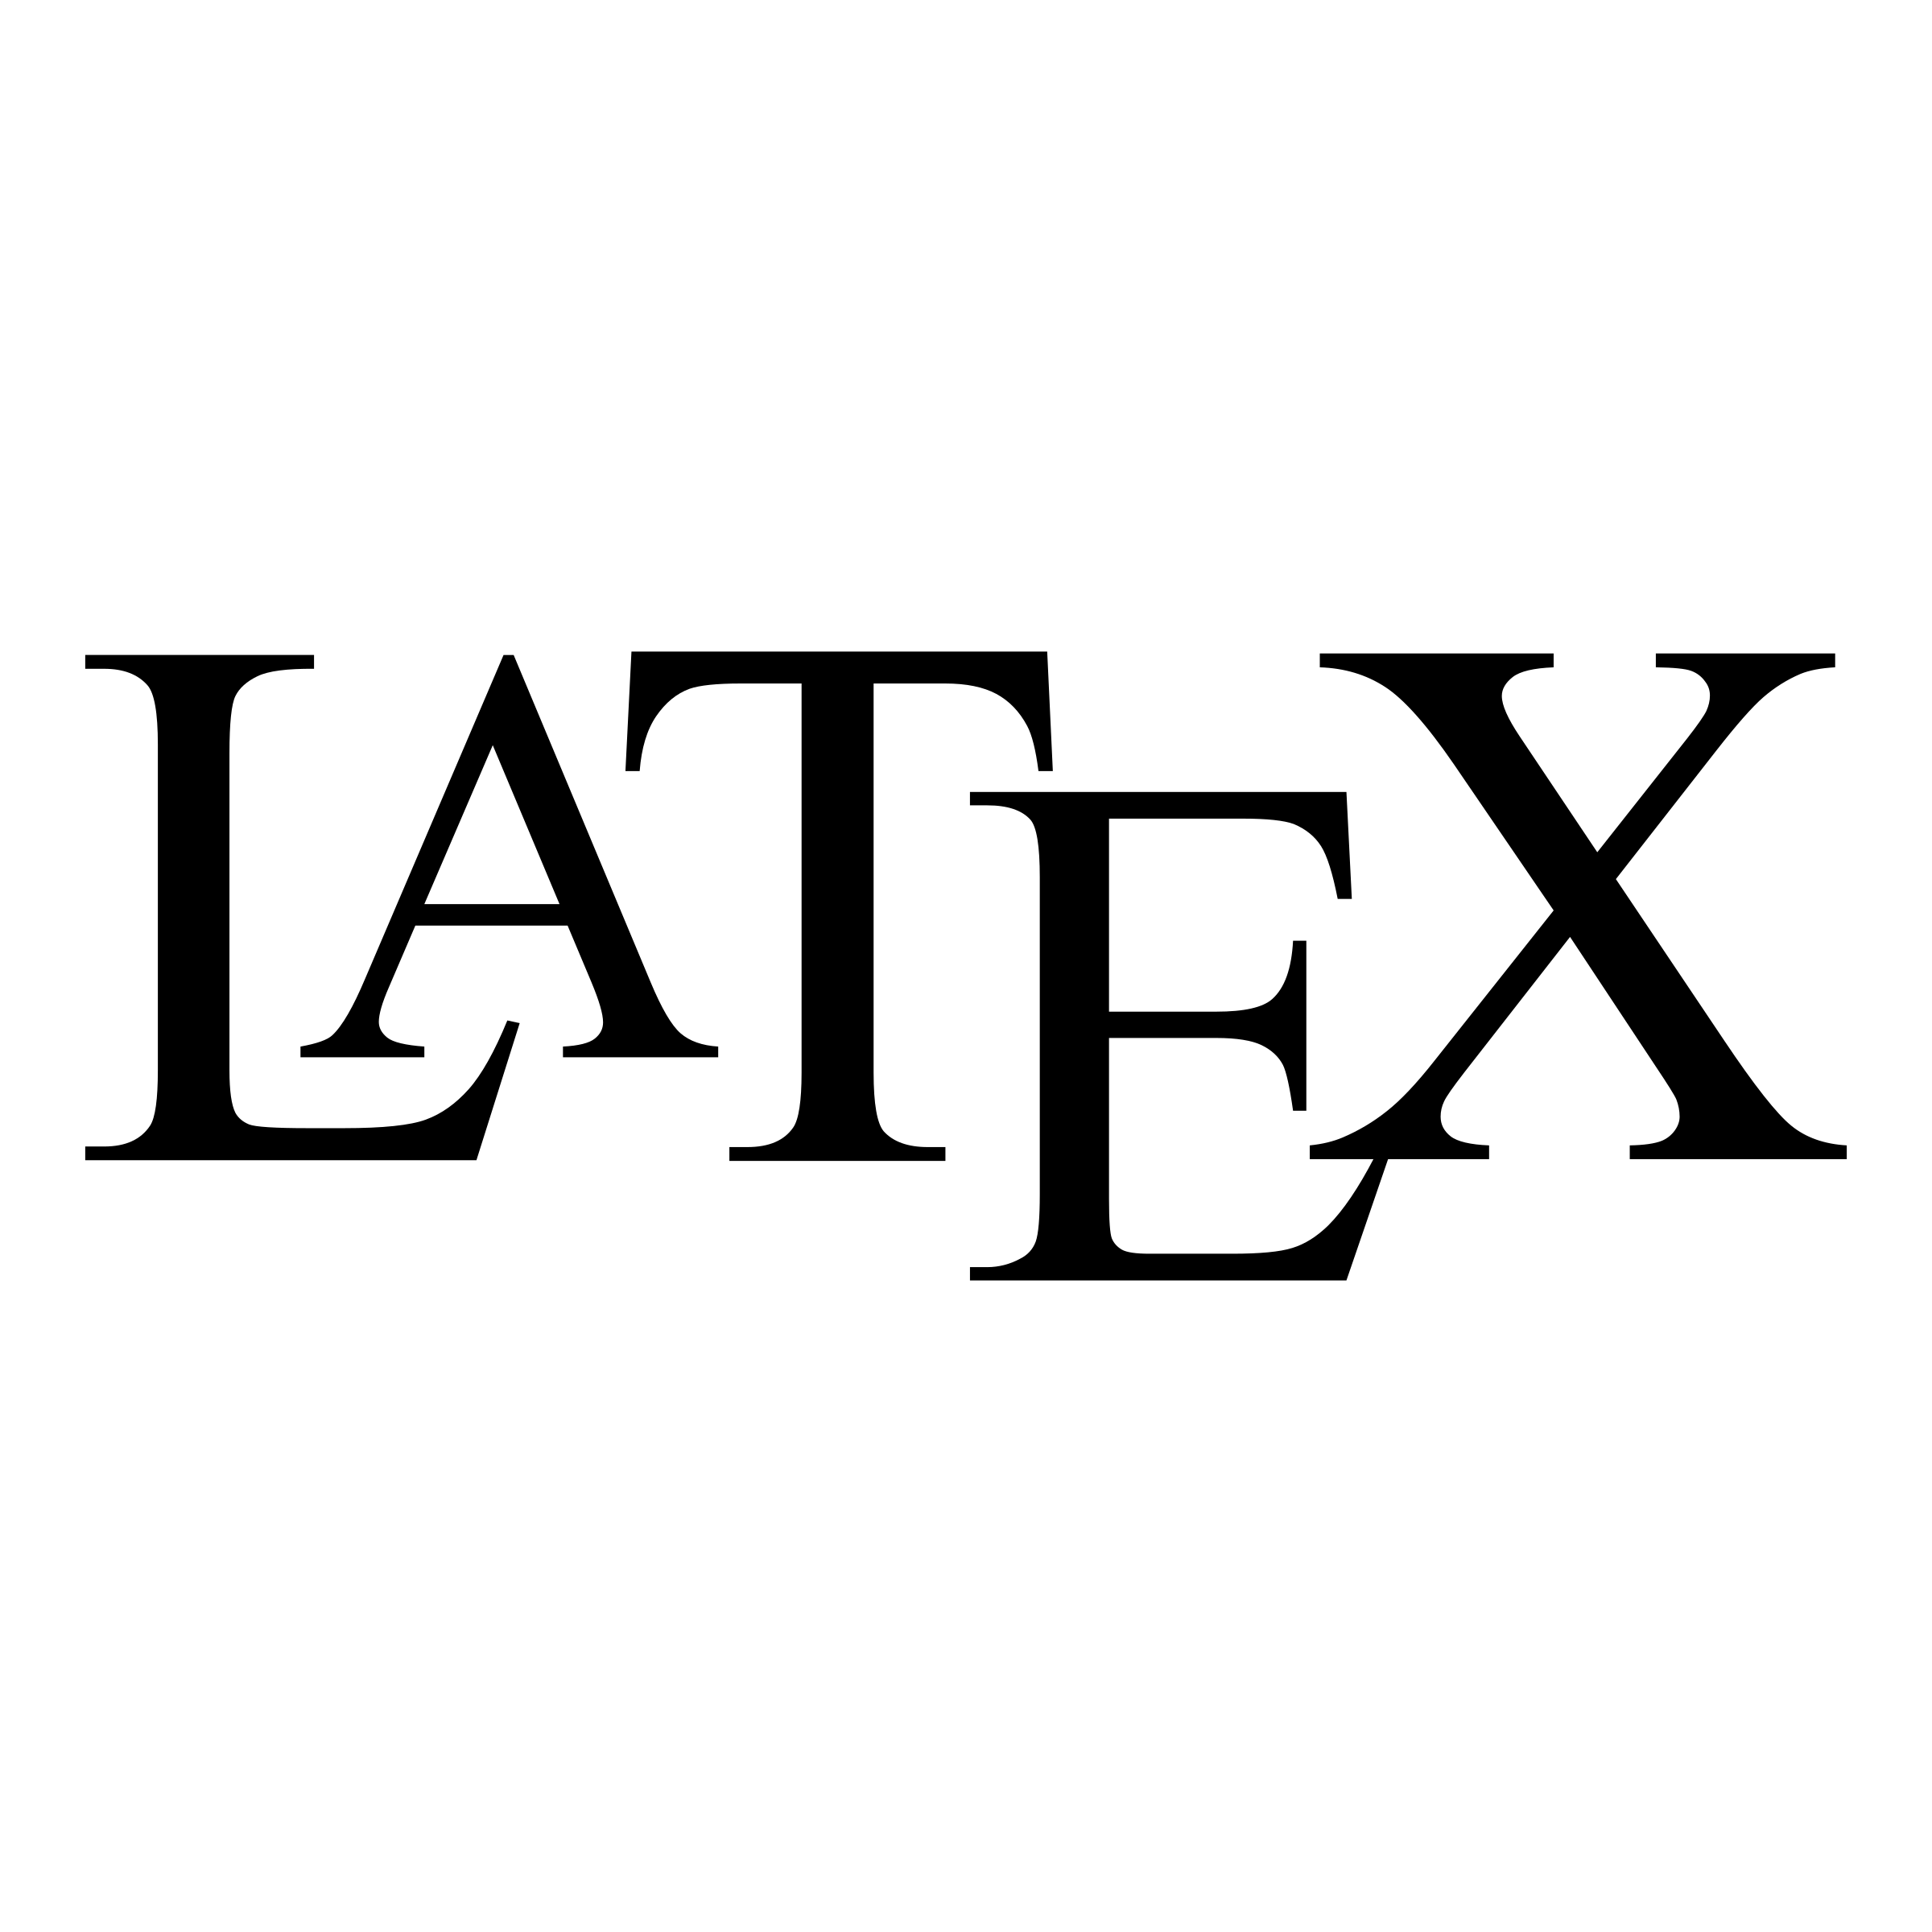
\includegraphics[width=0.4\textwidth]{LatexLogo.png}
    \qquad
    \parbox[b]{0.4\textwidth}{This is the comment on the figure.}
    \caption{Figure With Words Example}
\end{figure}

\paragraph{Figures Side By Side}
\begin{figure}[H]
    \centering
    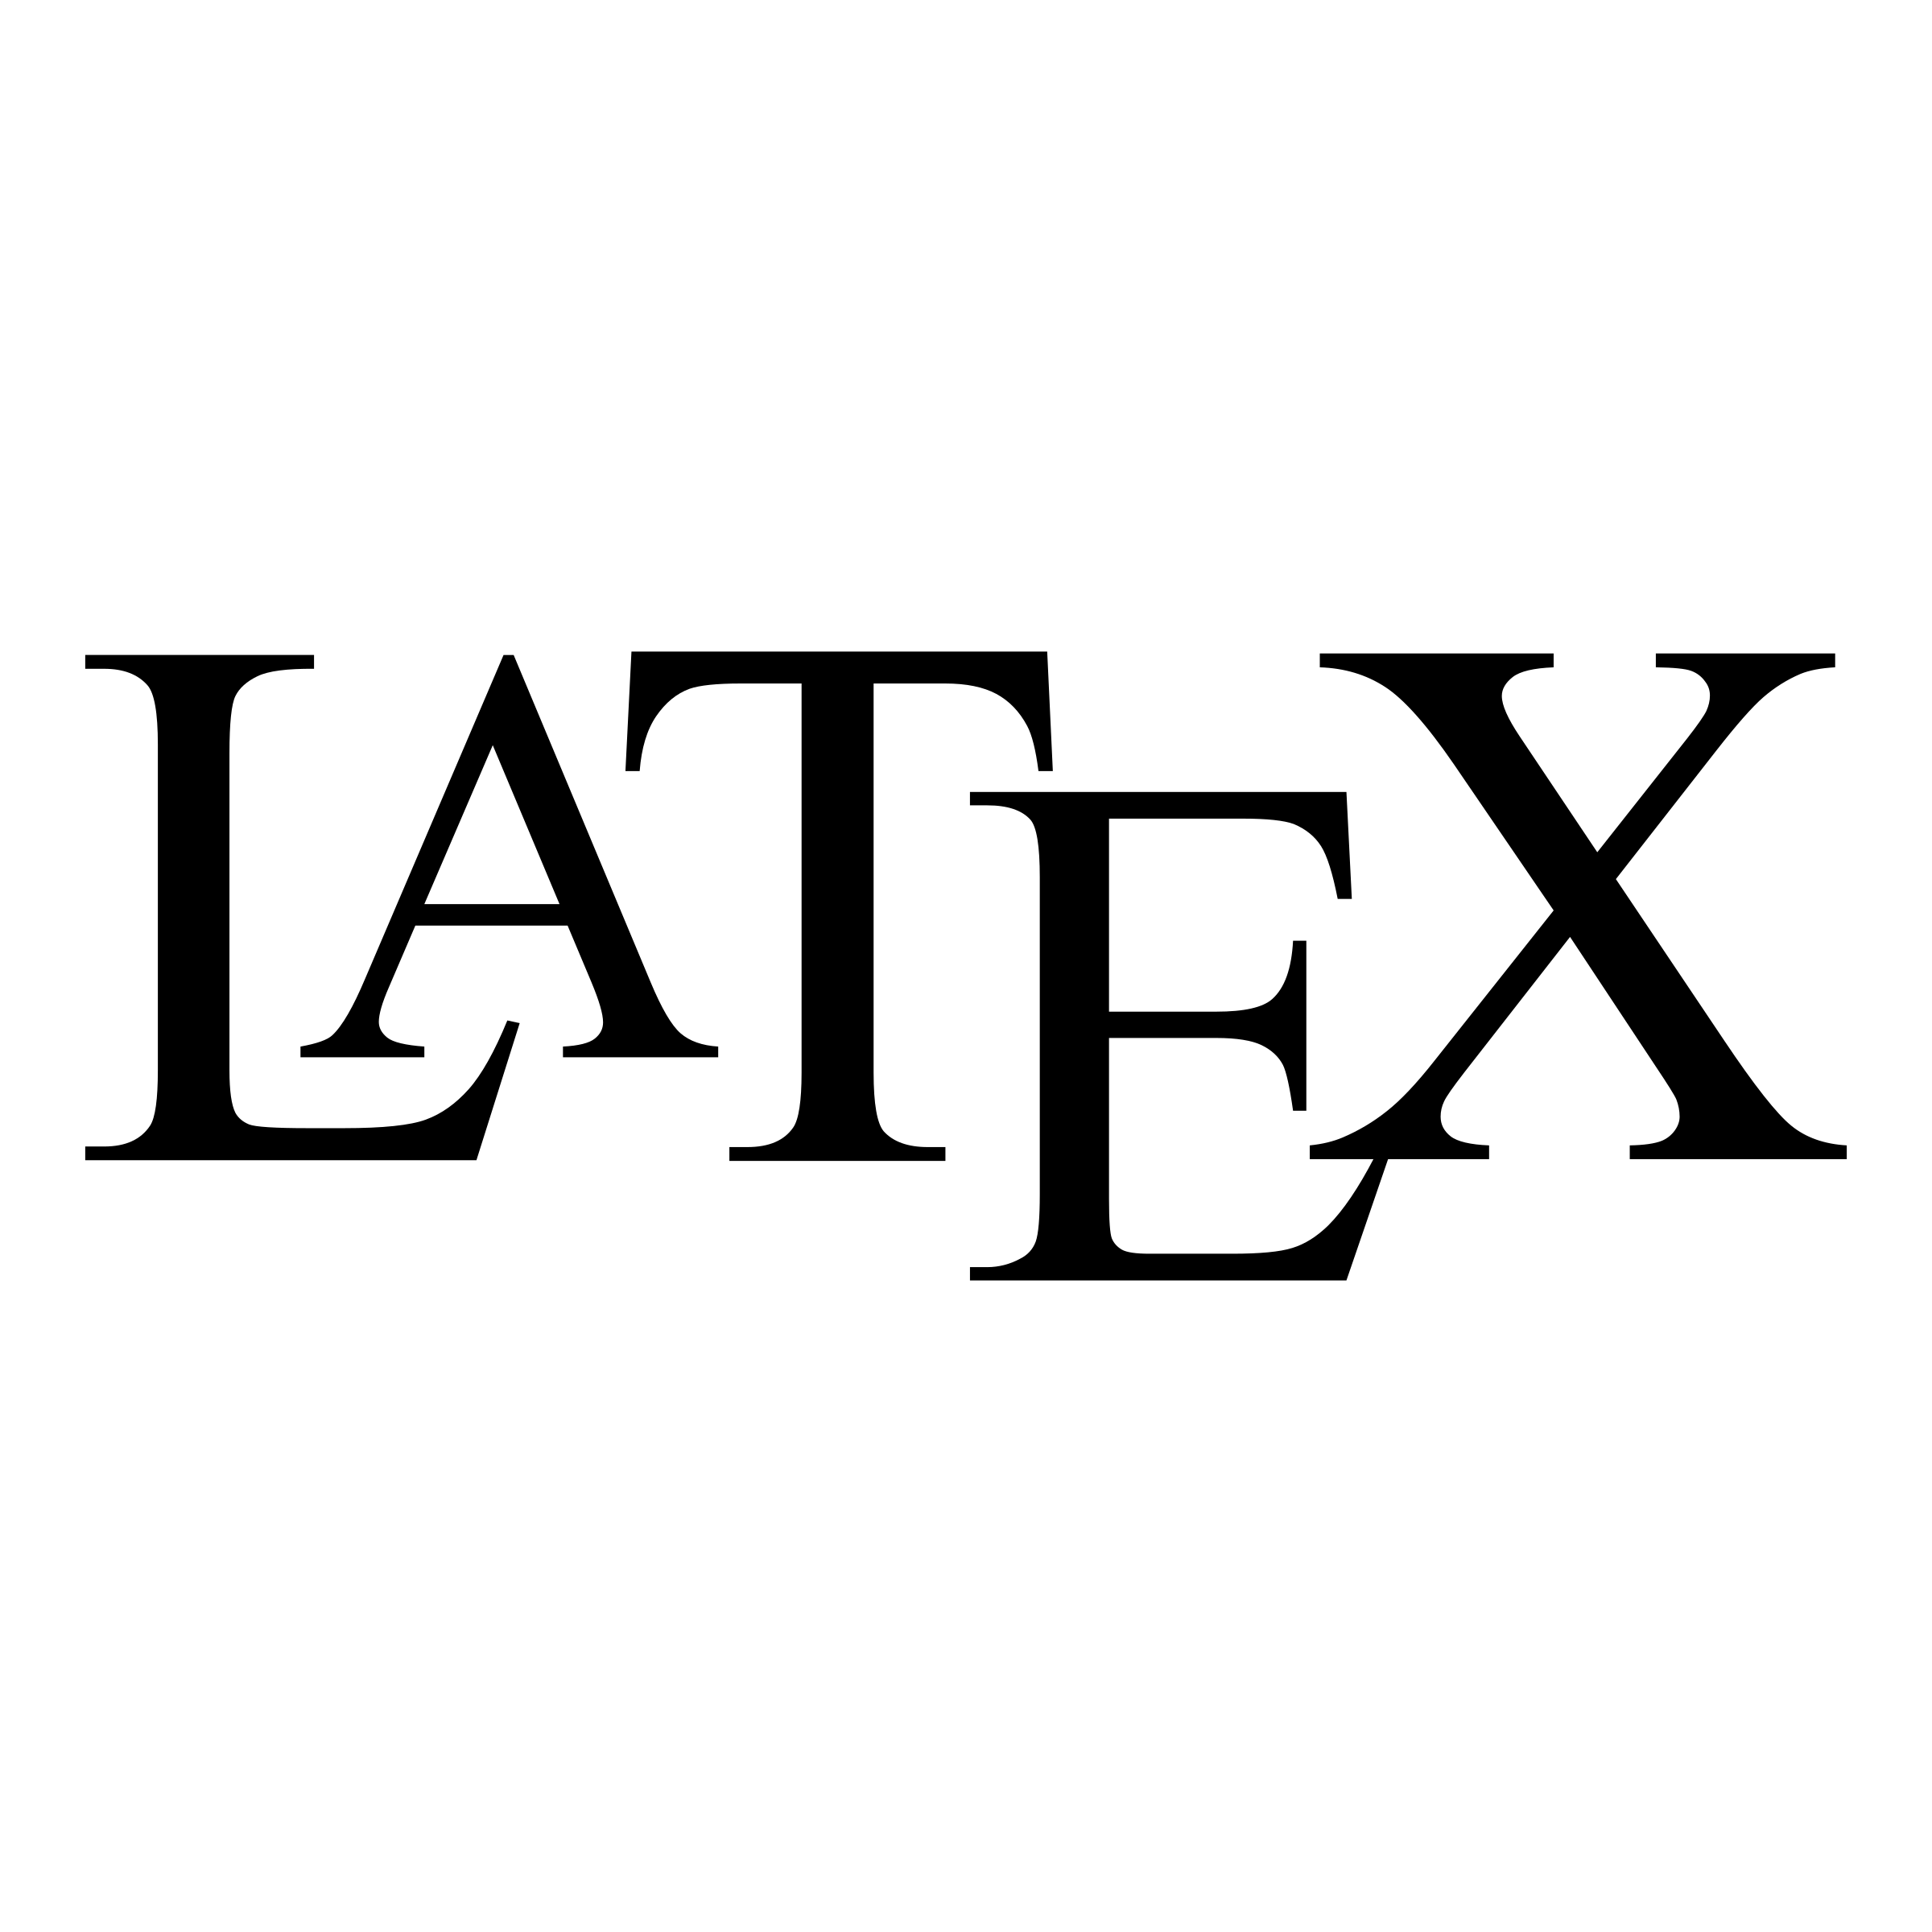
\includegraphics[width=0.4\textwidth]{LatexLogo.png}
    \qquad
    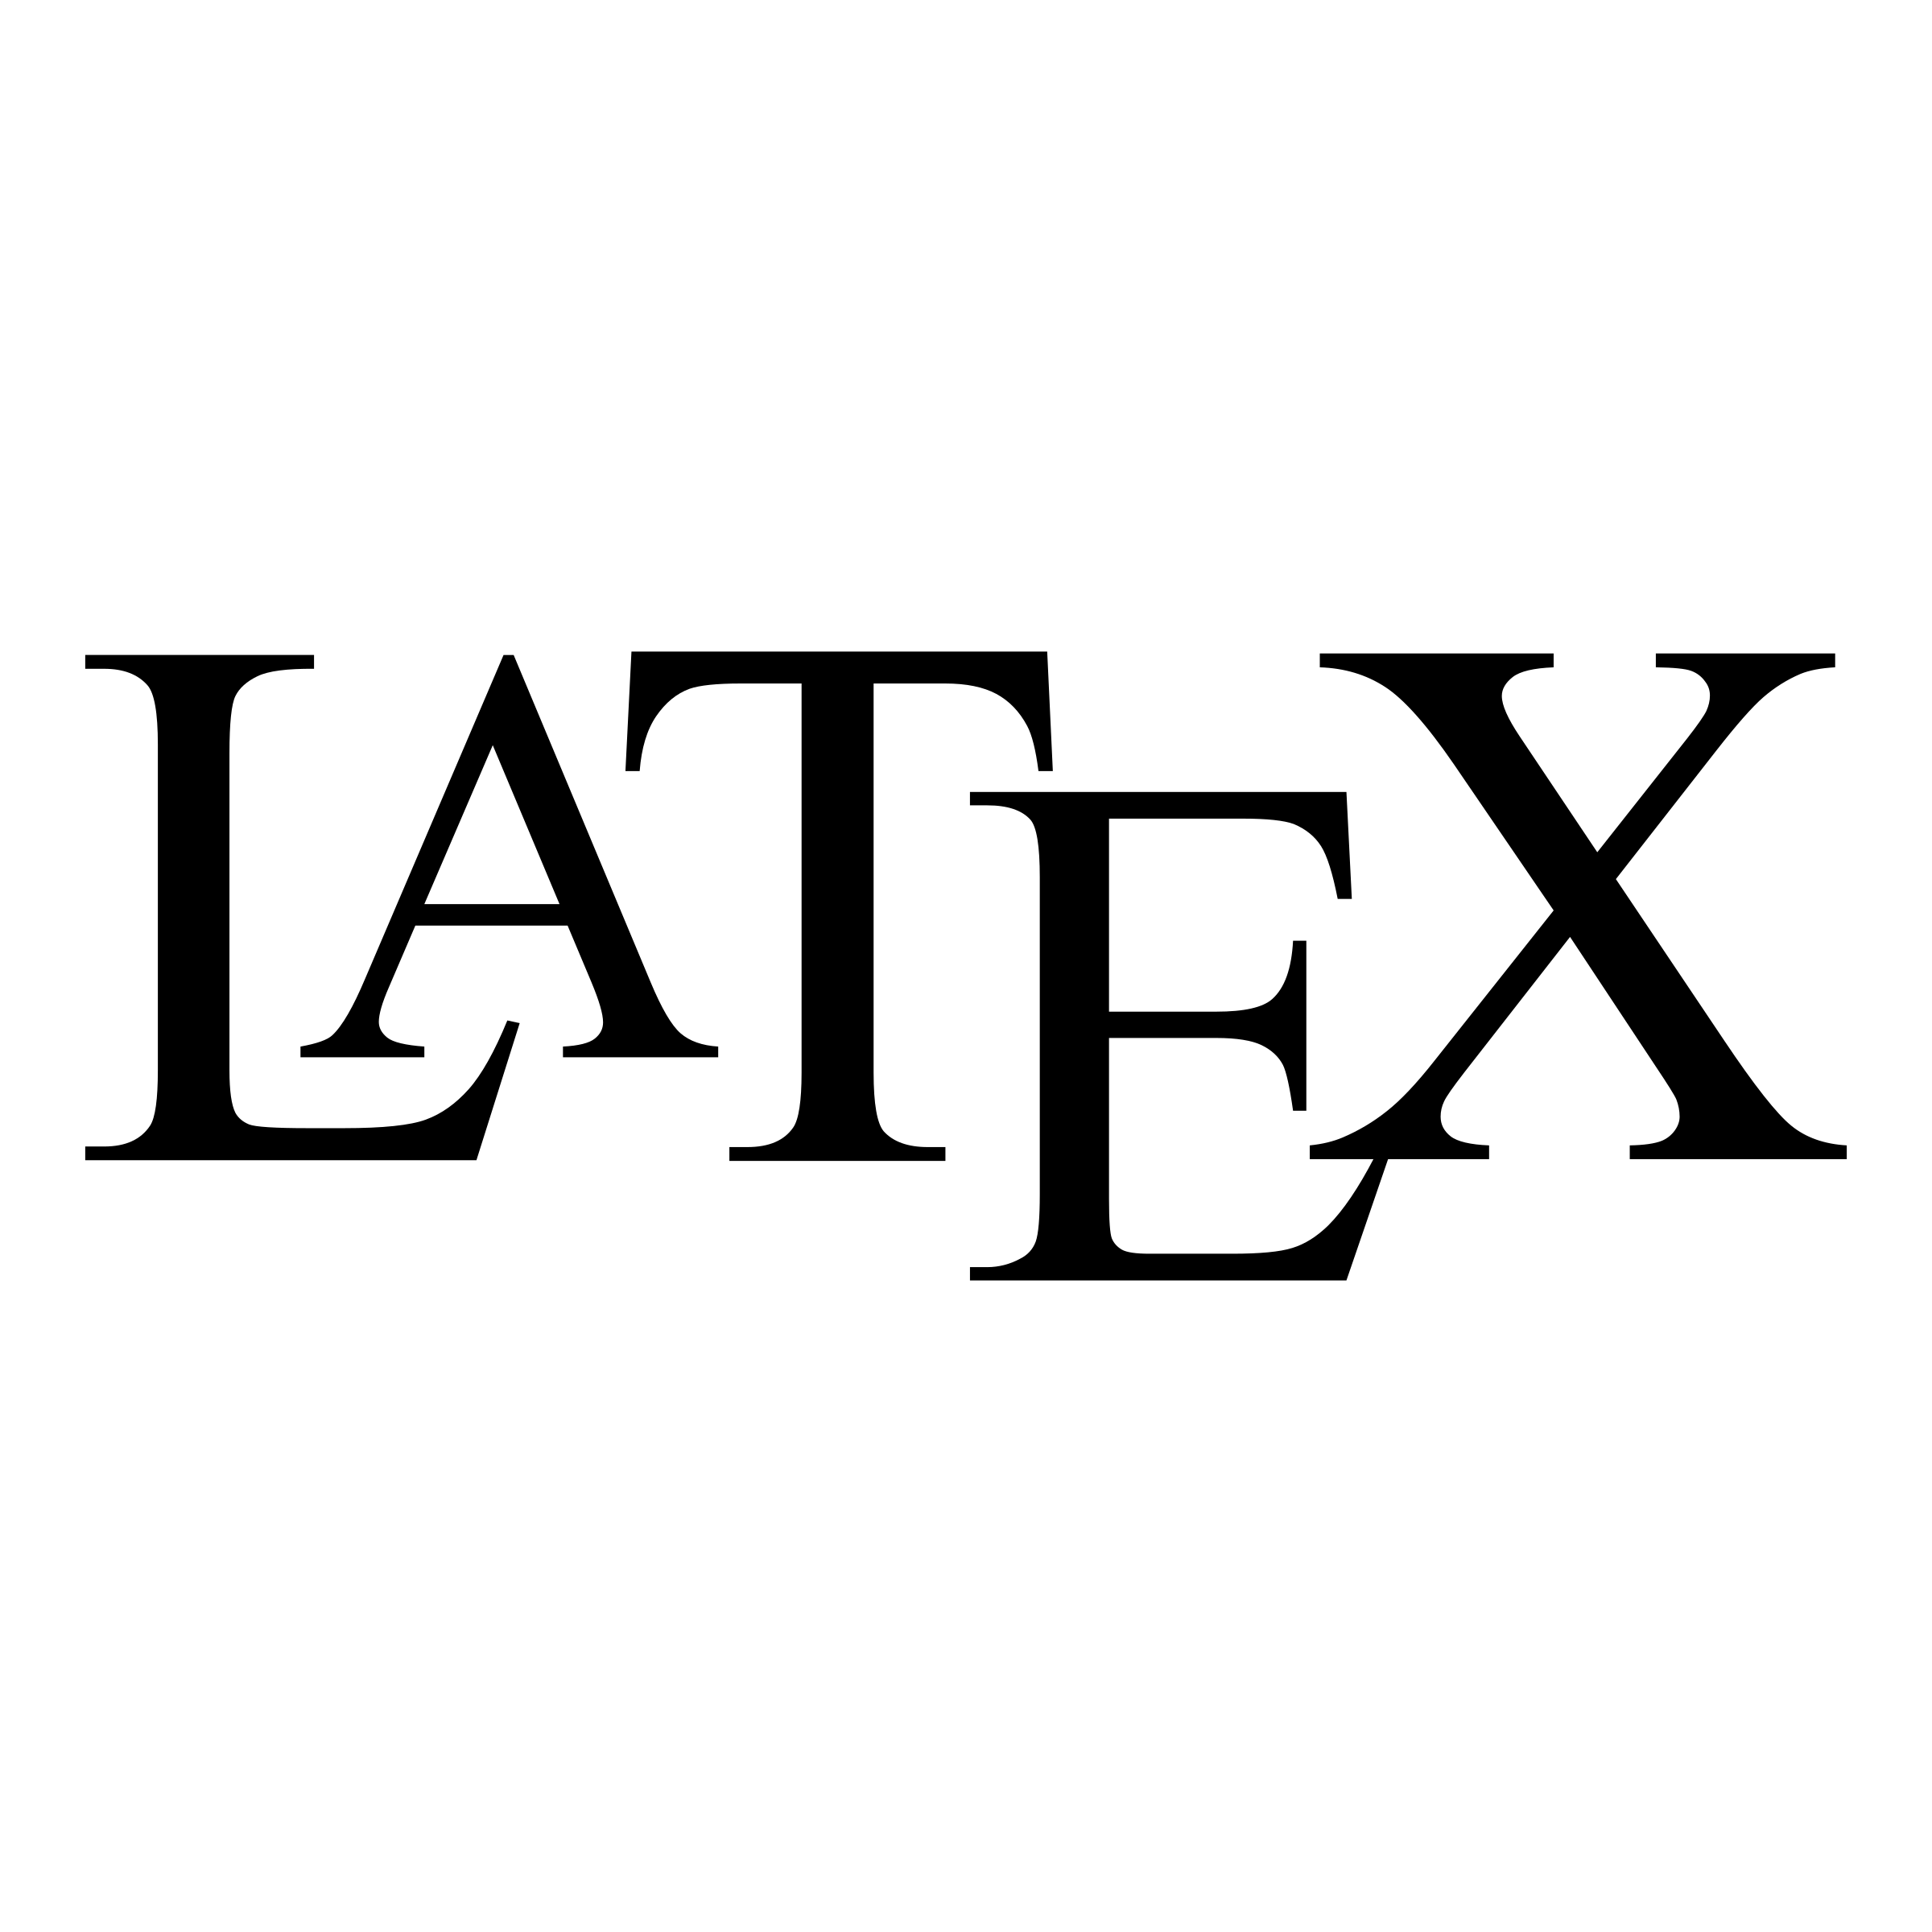
\includegraphics[width=0.4\textwidth]{LatexLogo.png}
    \caption{Figure Side By Side Example}
\end{figure}

\paragraph{Captions For Side By Side}
\begin{figure}[H]
    \caption{Title For Both}
    \parbox[b]{0.5\textwidth}{\centering
        \caption{Title For Left}
        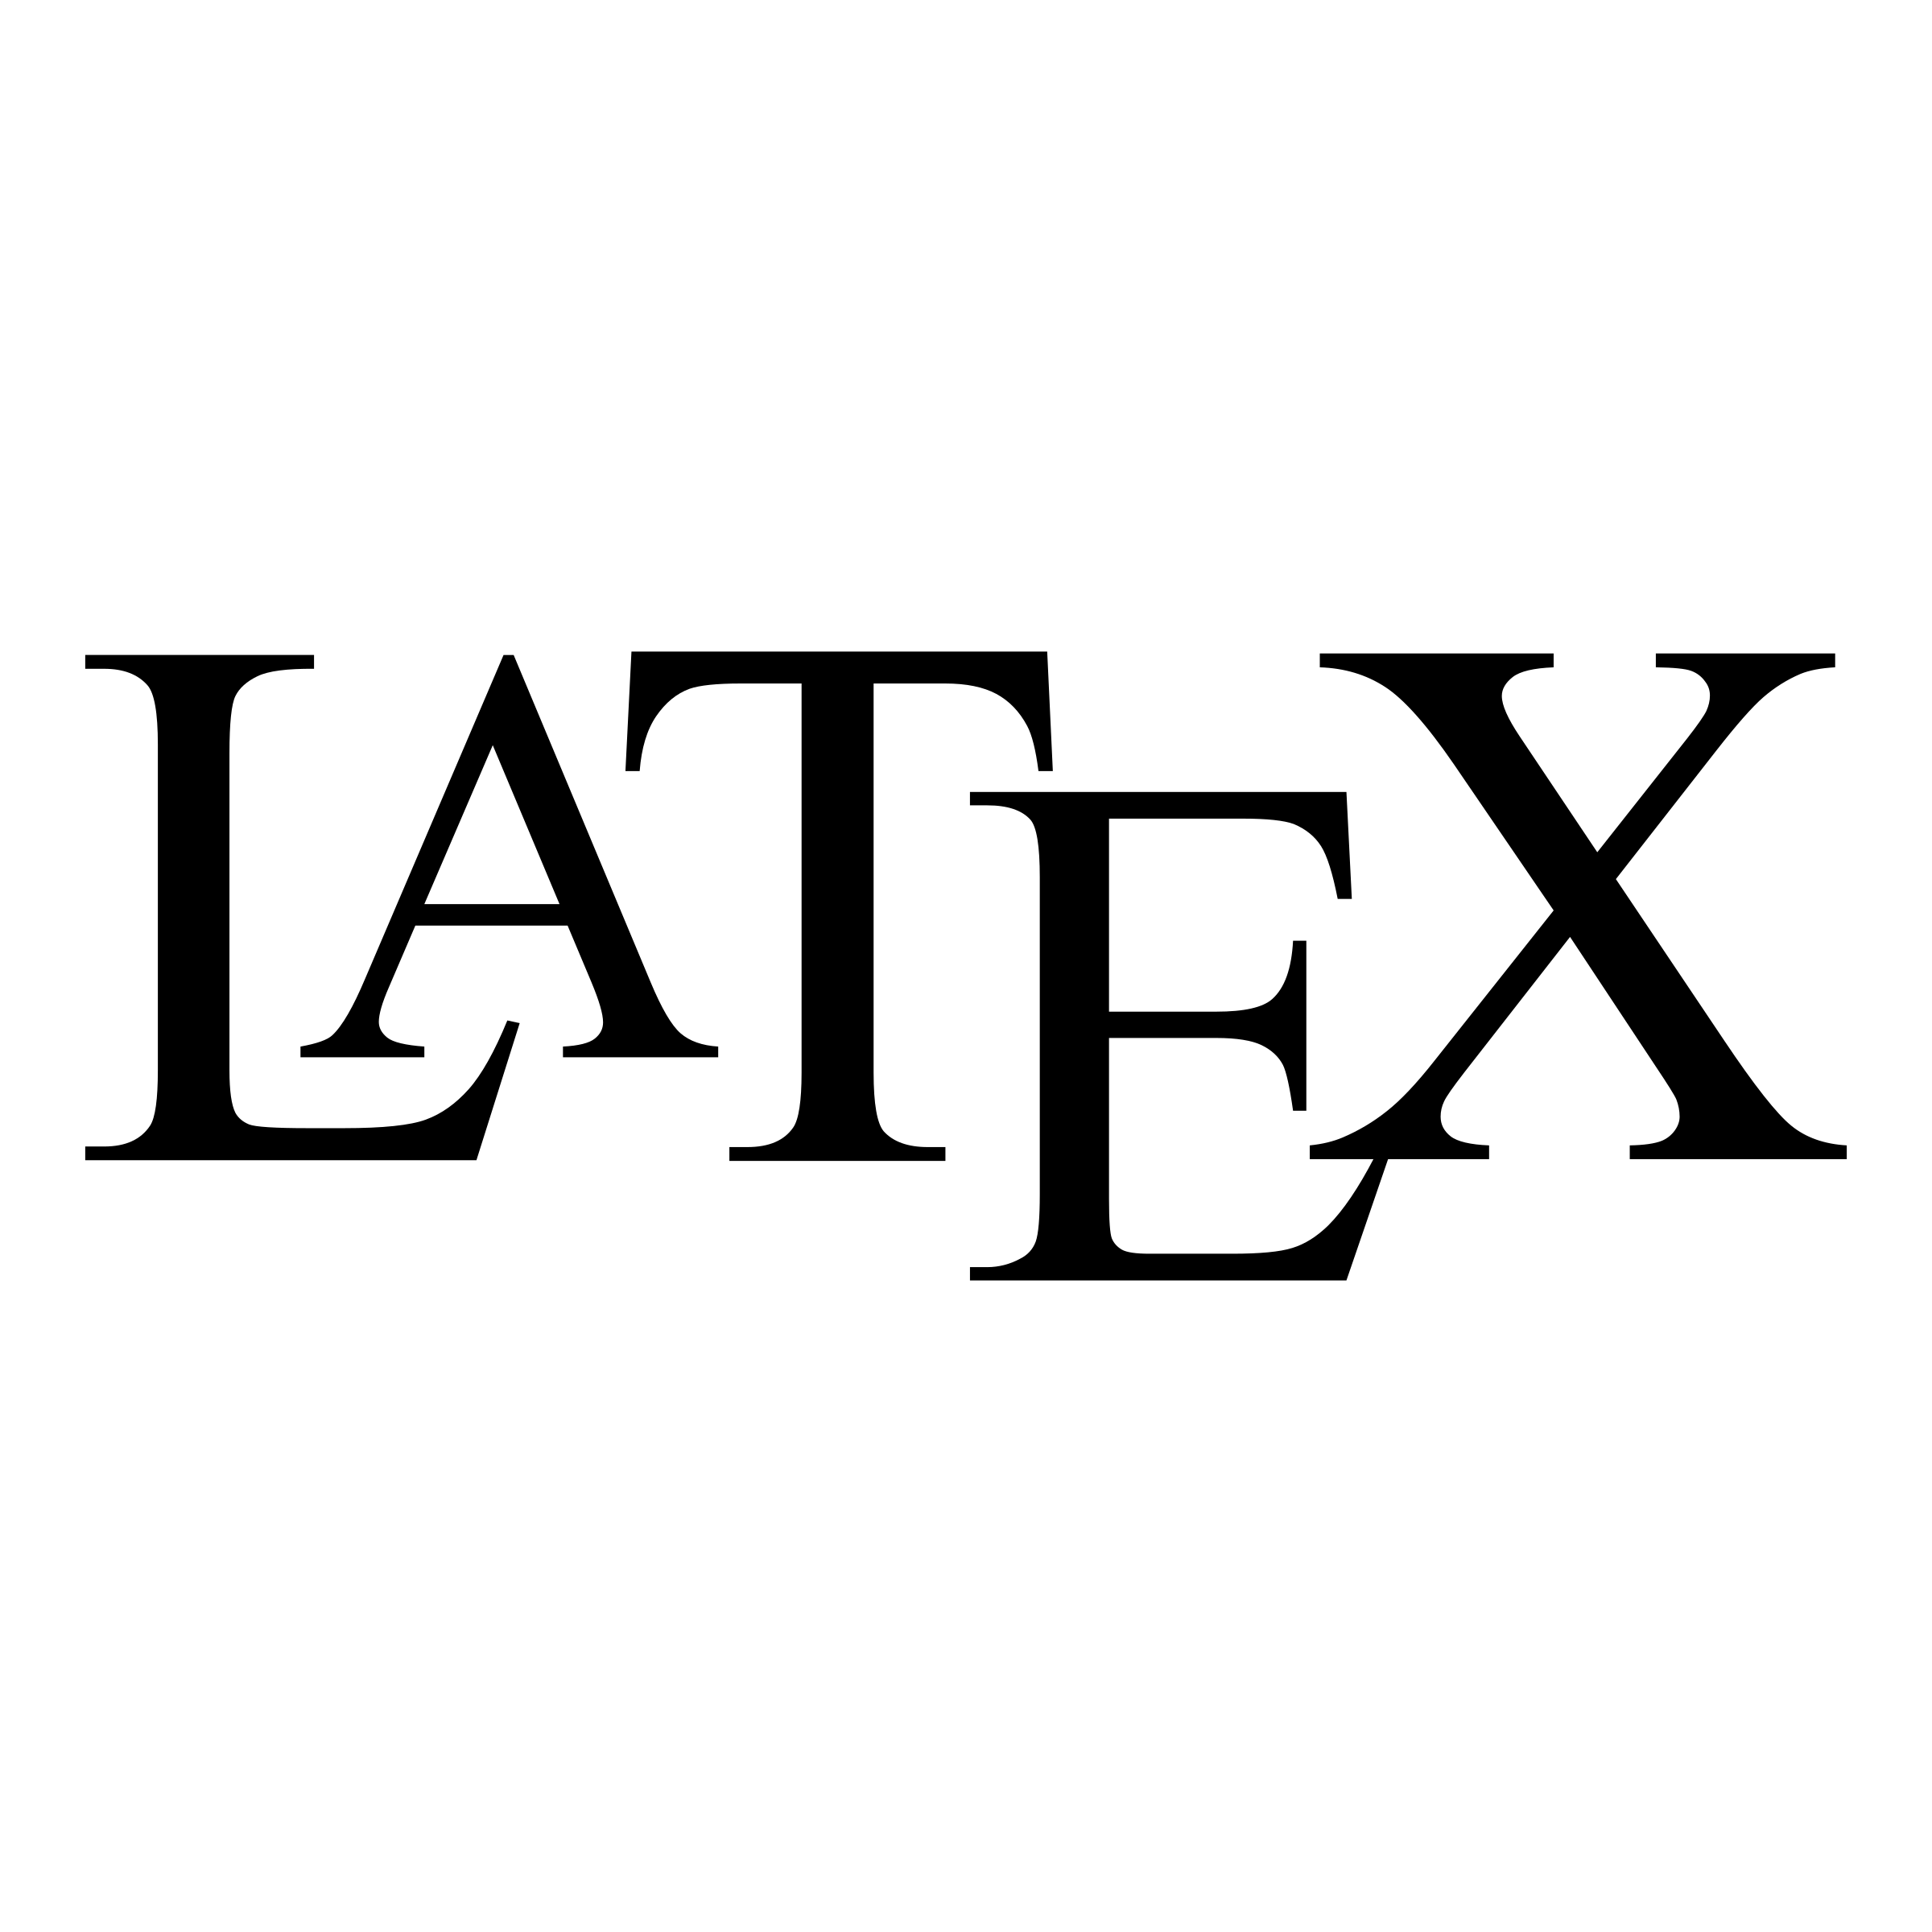
\includegraphics[width=0.4\textwidth]{LatexLogo.png}}
    \parbox[b]{0.5\textwidth}{\centering
        \caption{Title For Right}
        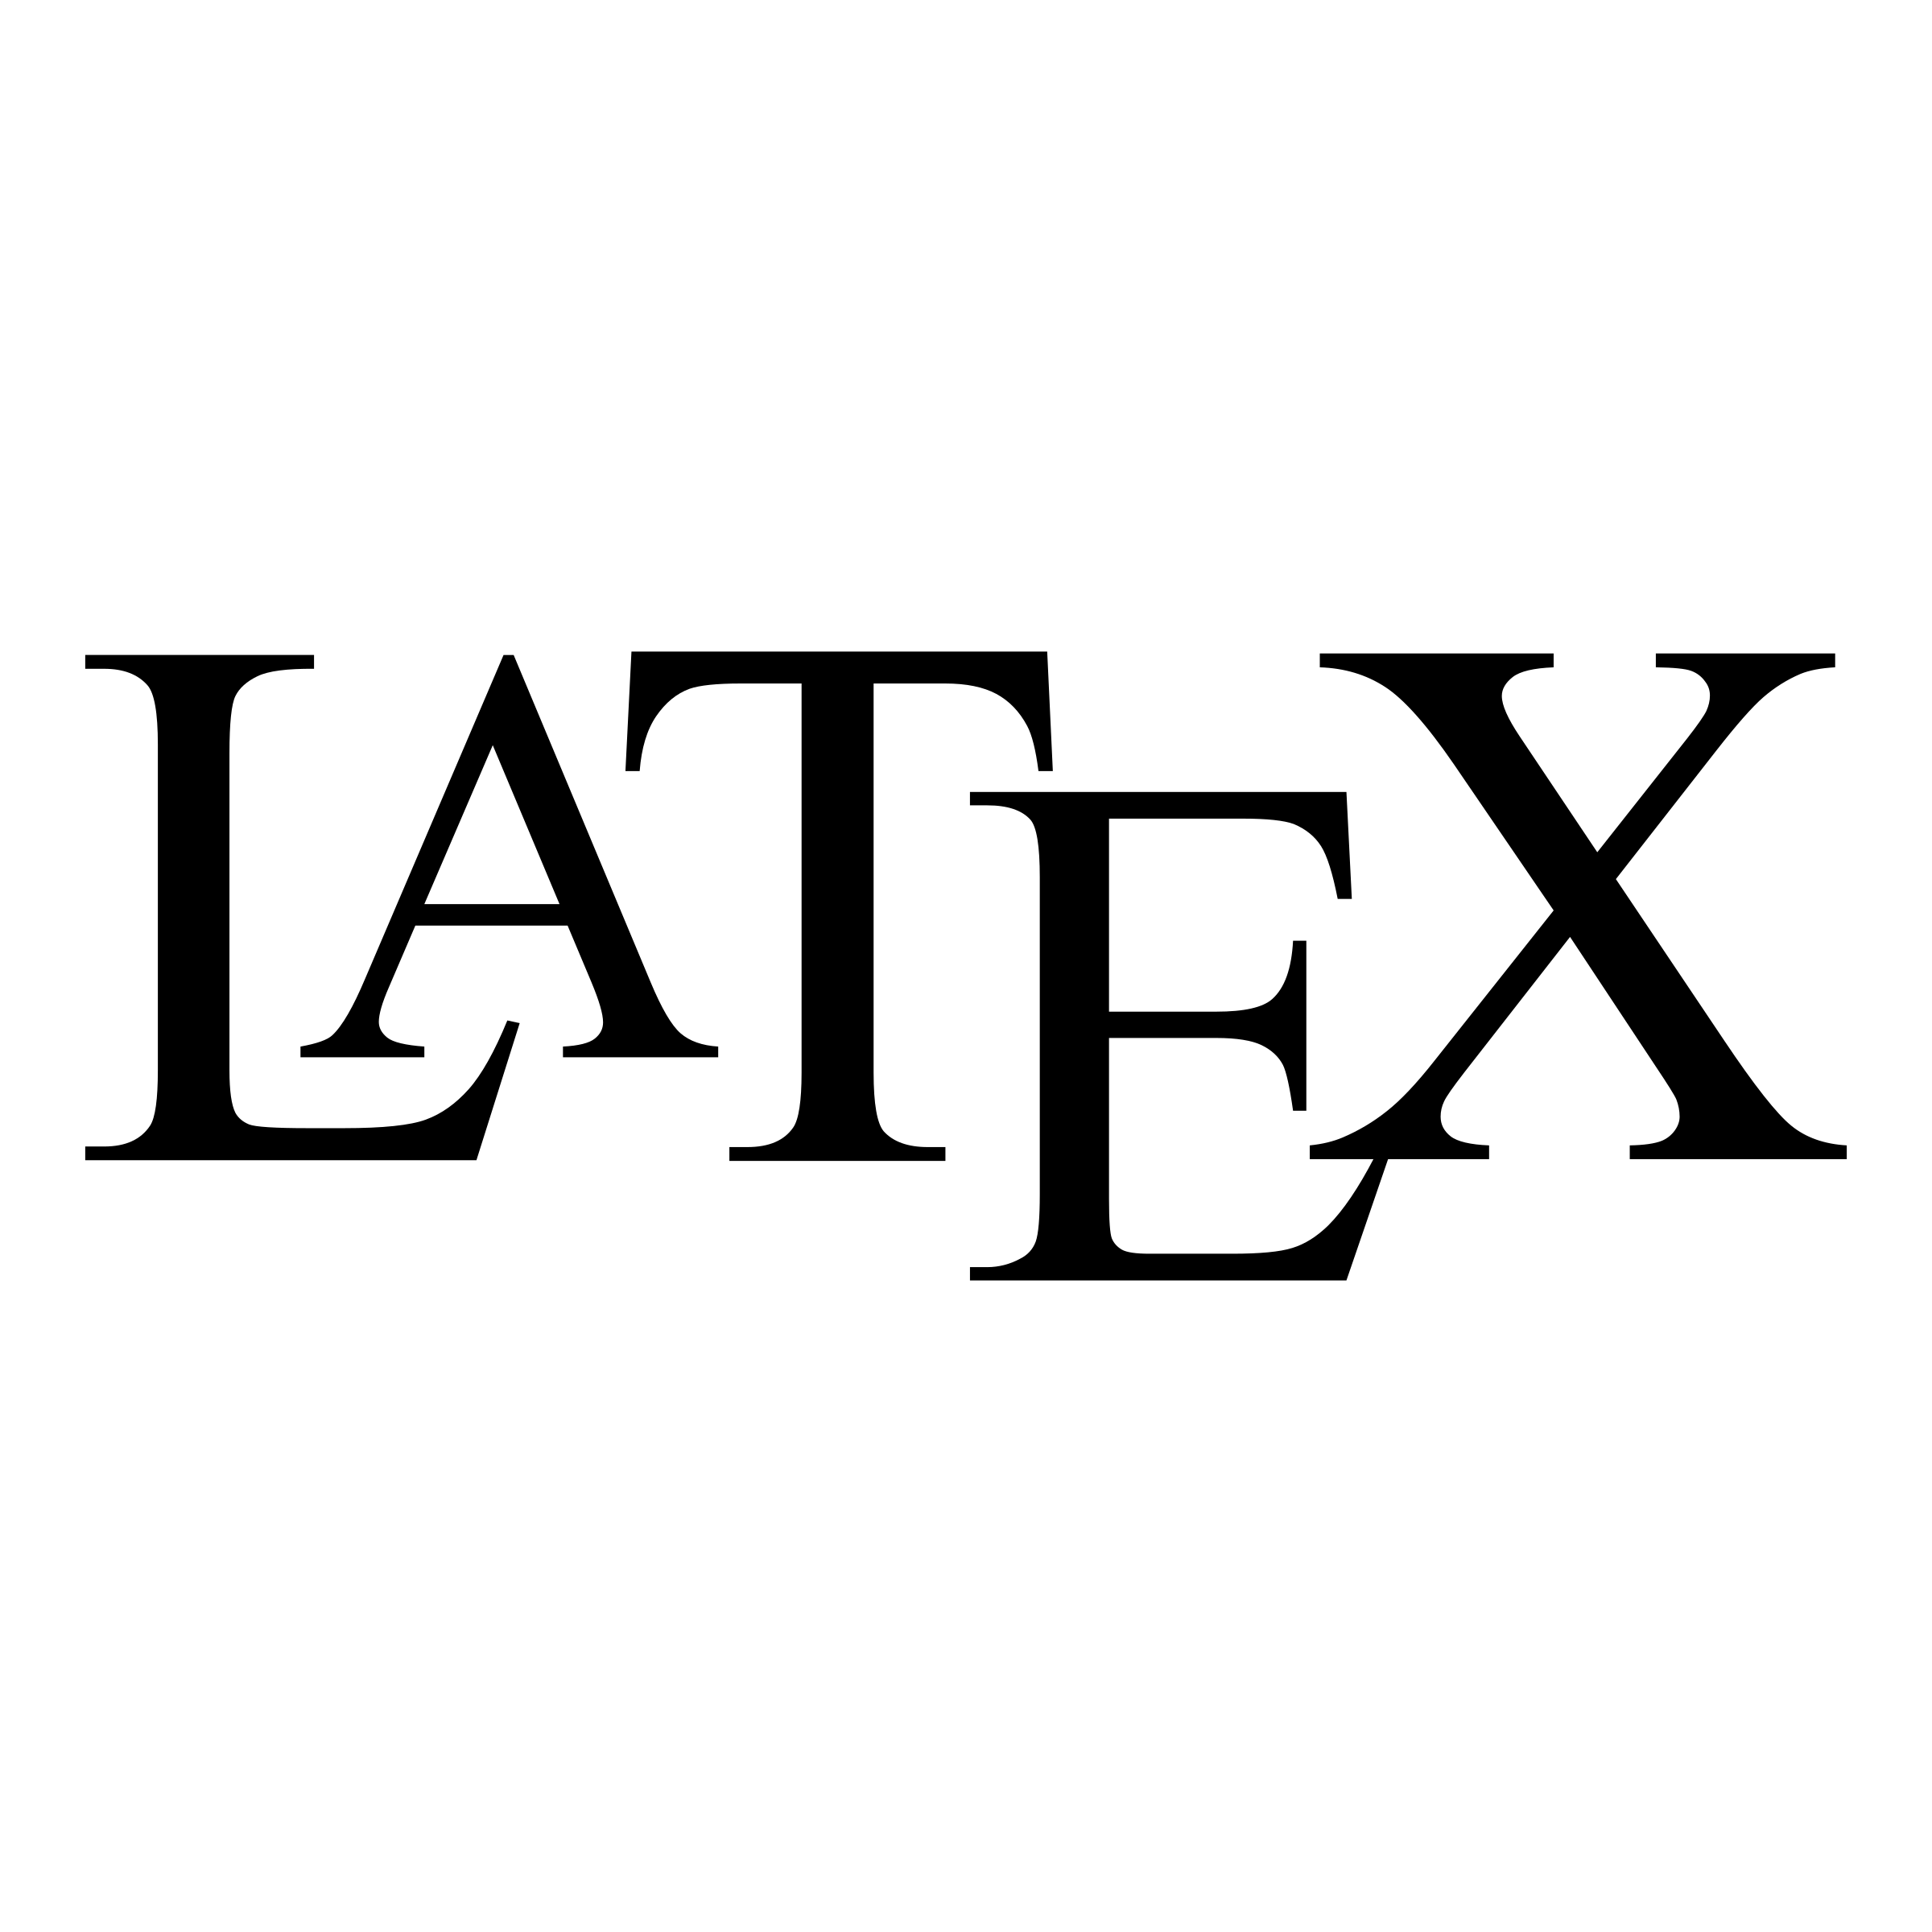
\includegraphics[width=0.4\textwidth]{LatexLogo.png}}
\end{figure}

\begin{figure}[H]
    % must usepackage subcaption
    \caption{Title For Both}
    \begin{subfigure}[b]{0.5\textwidth}
        \centering
        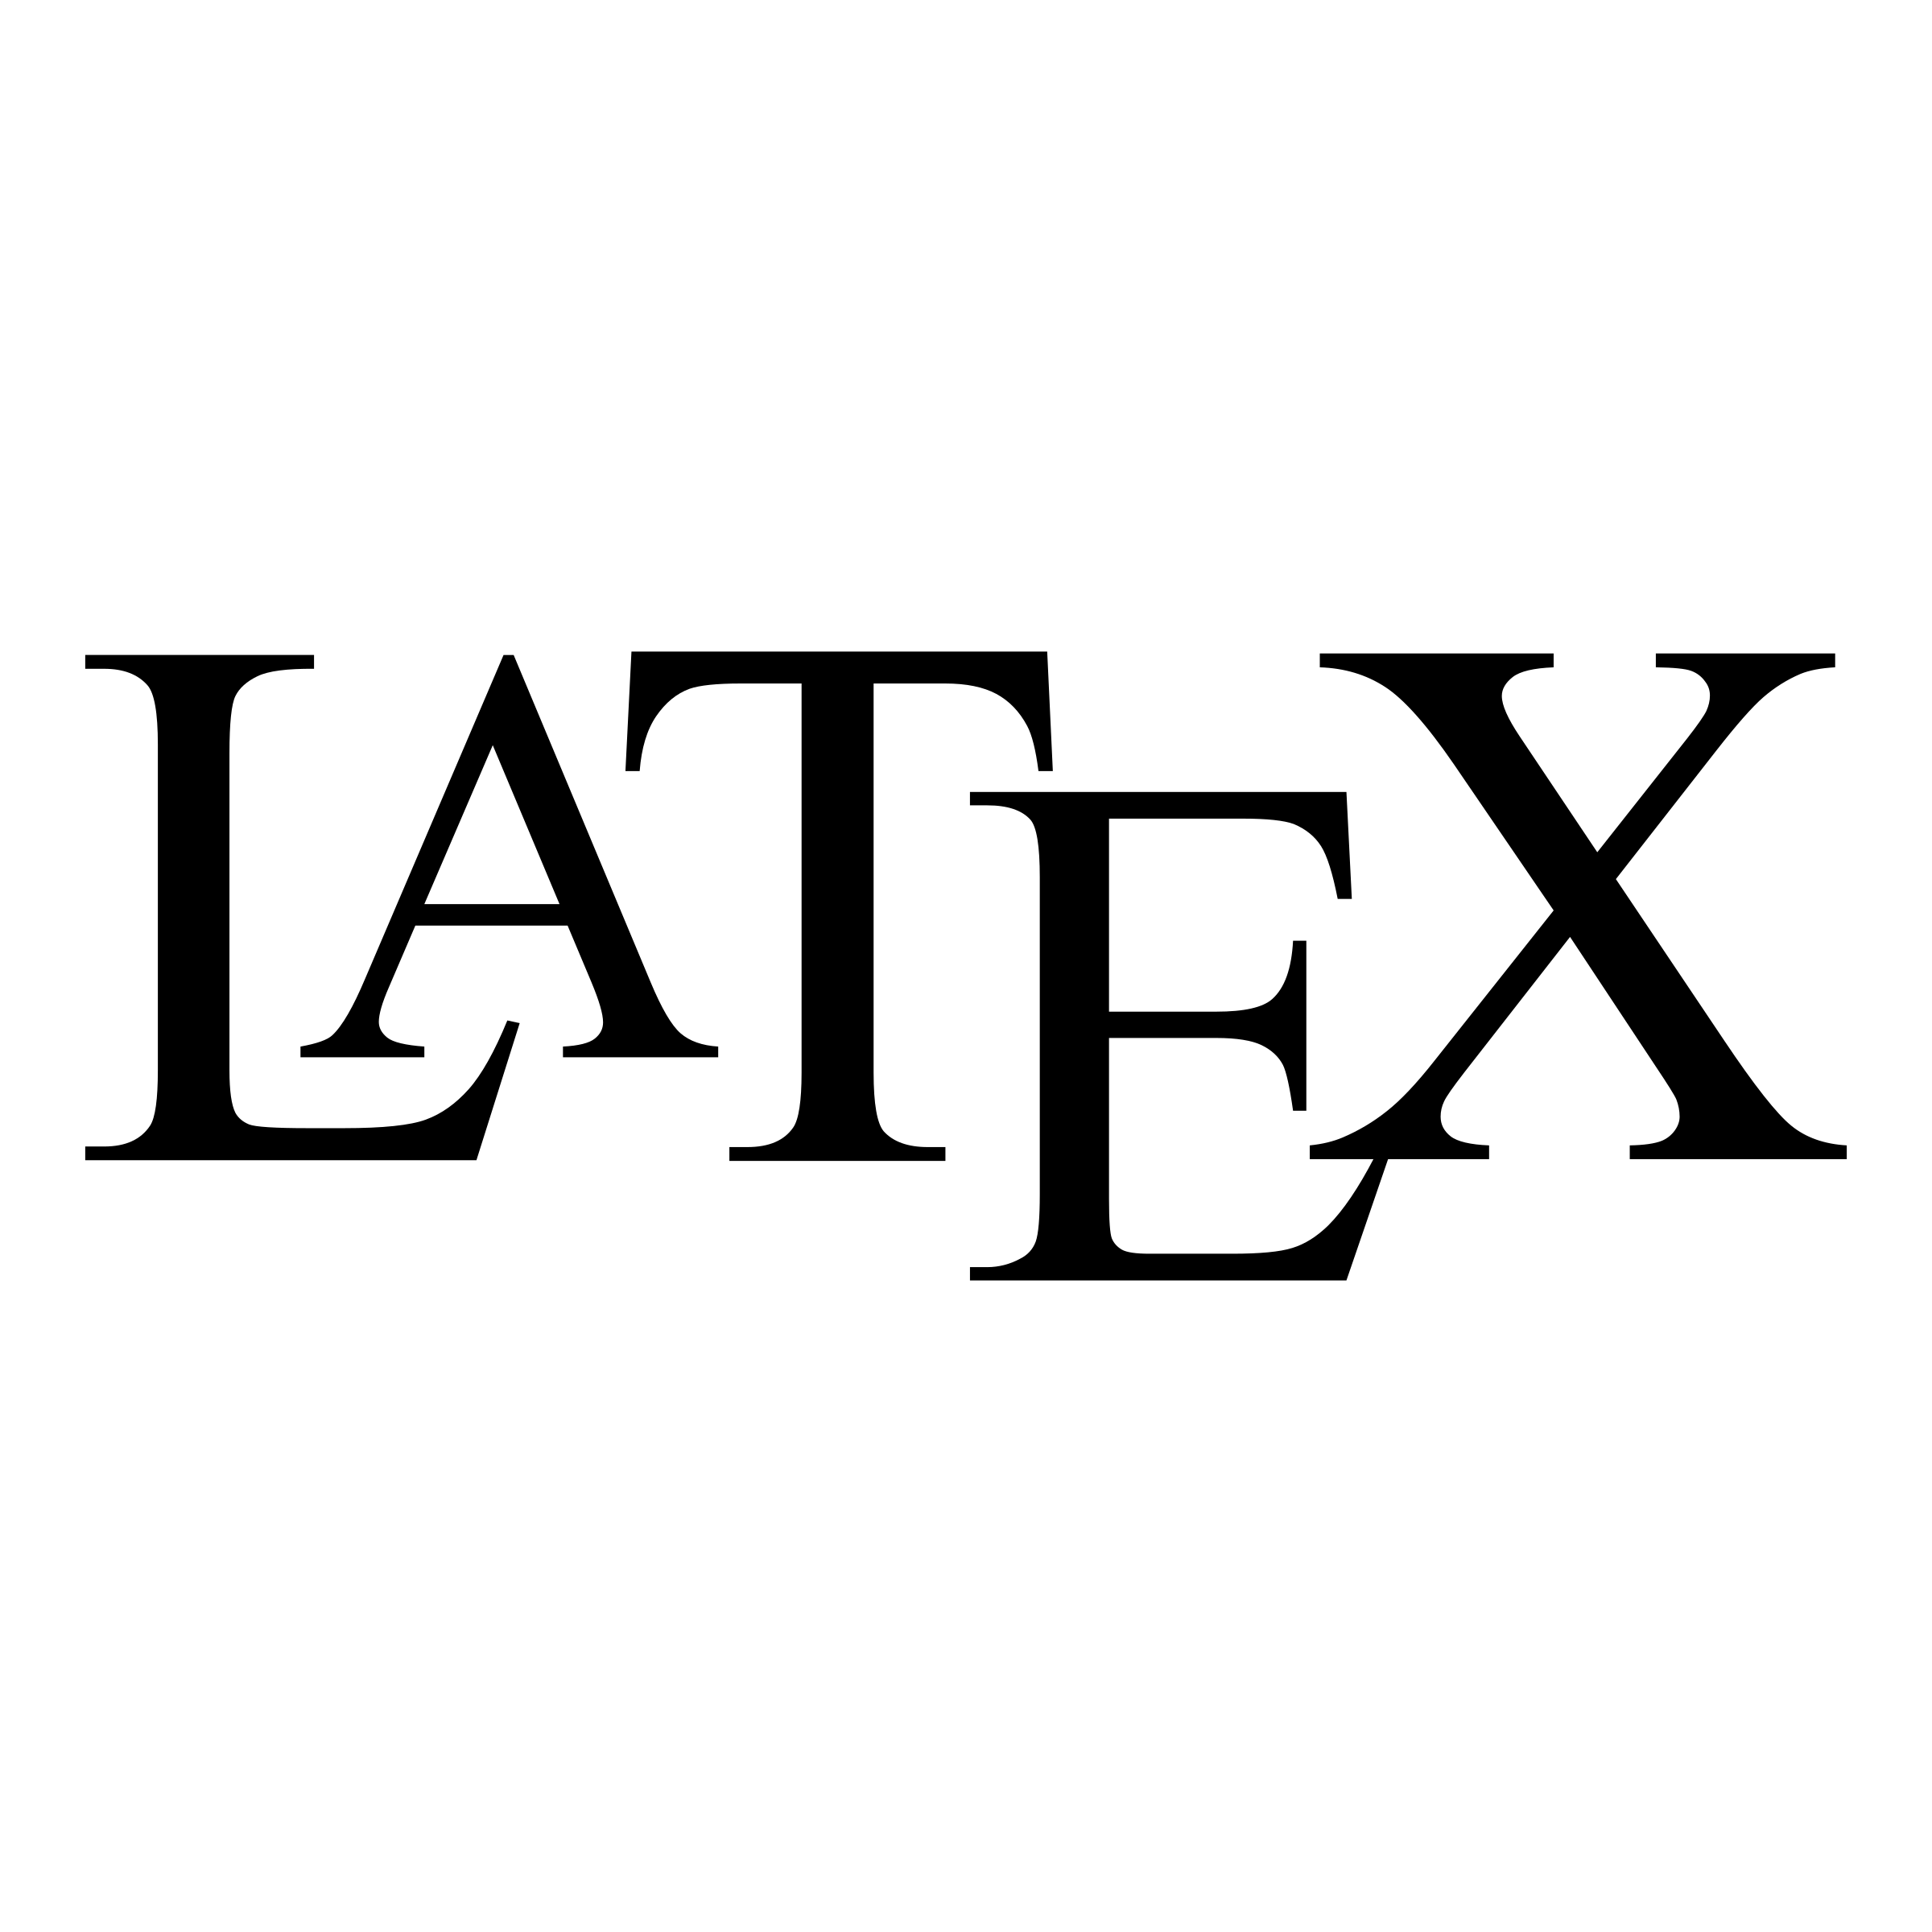
\includegraphics[width=0.4\textwidth]{LatexLogo.png}
        \caption{Title For Left}
    \end{subfigure}
    \begin{subfigure}[b]{0.5\textwidth}
        \centering
        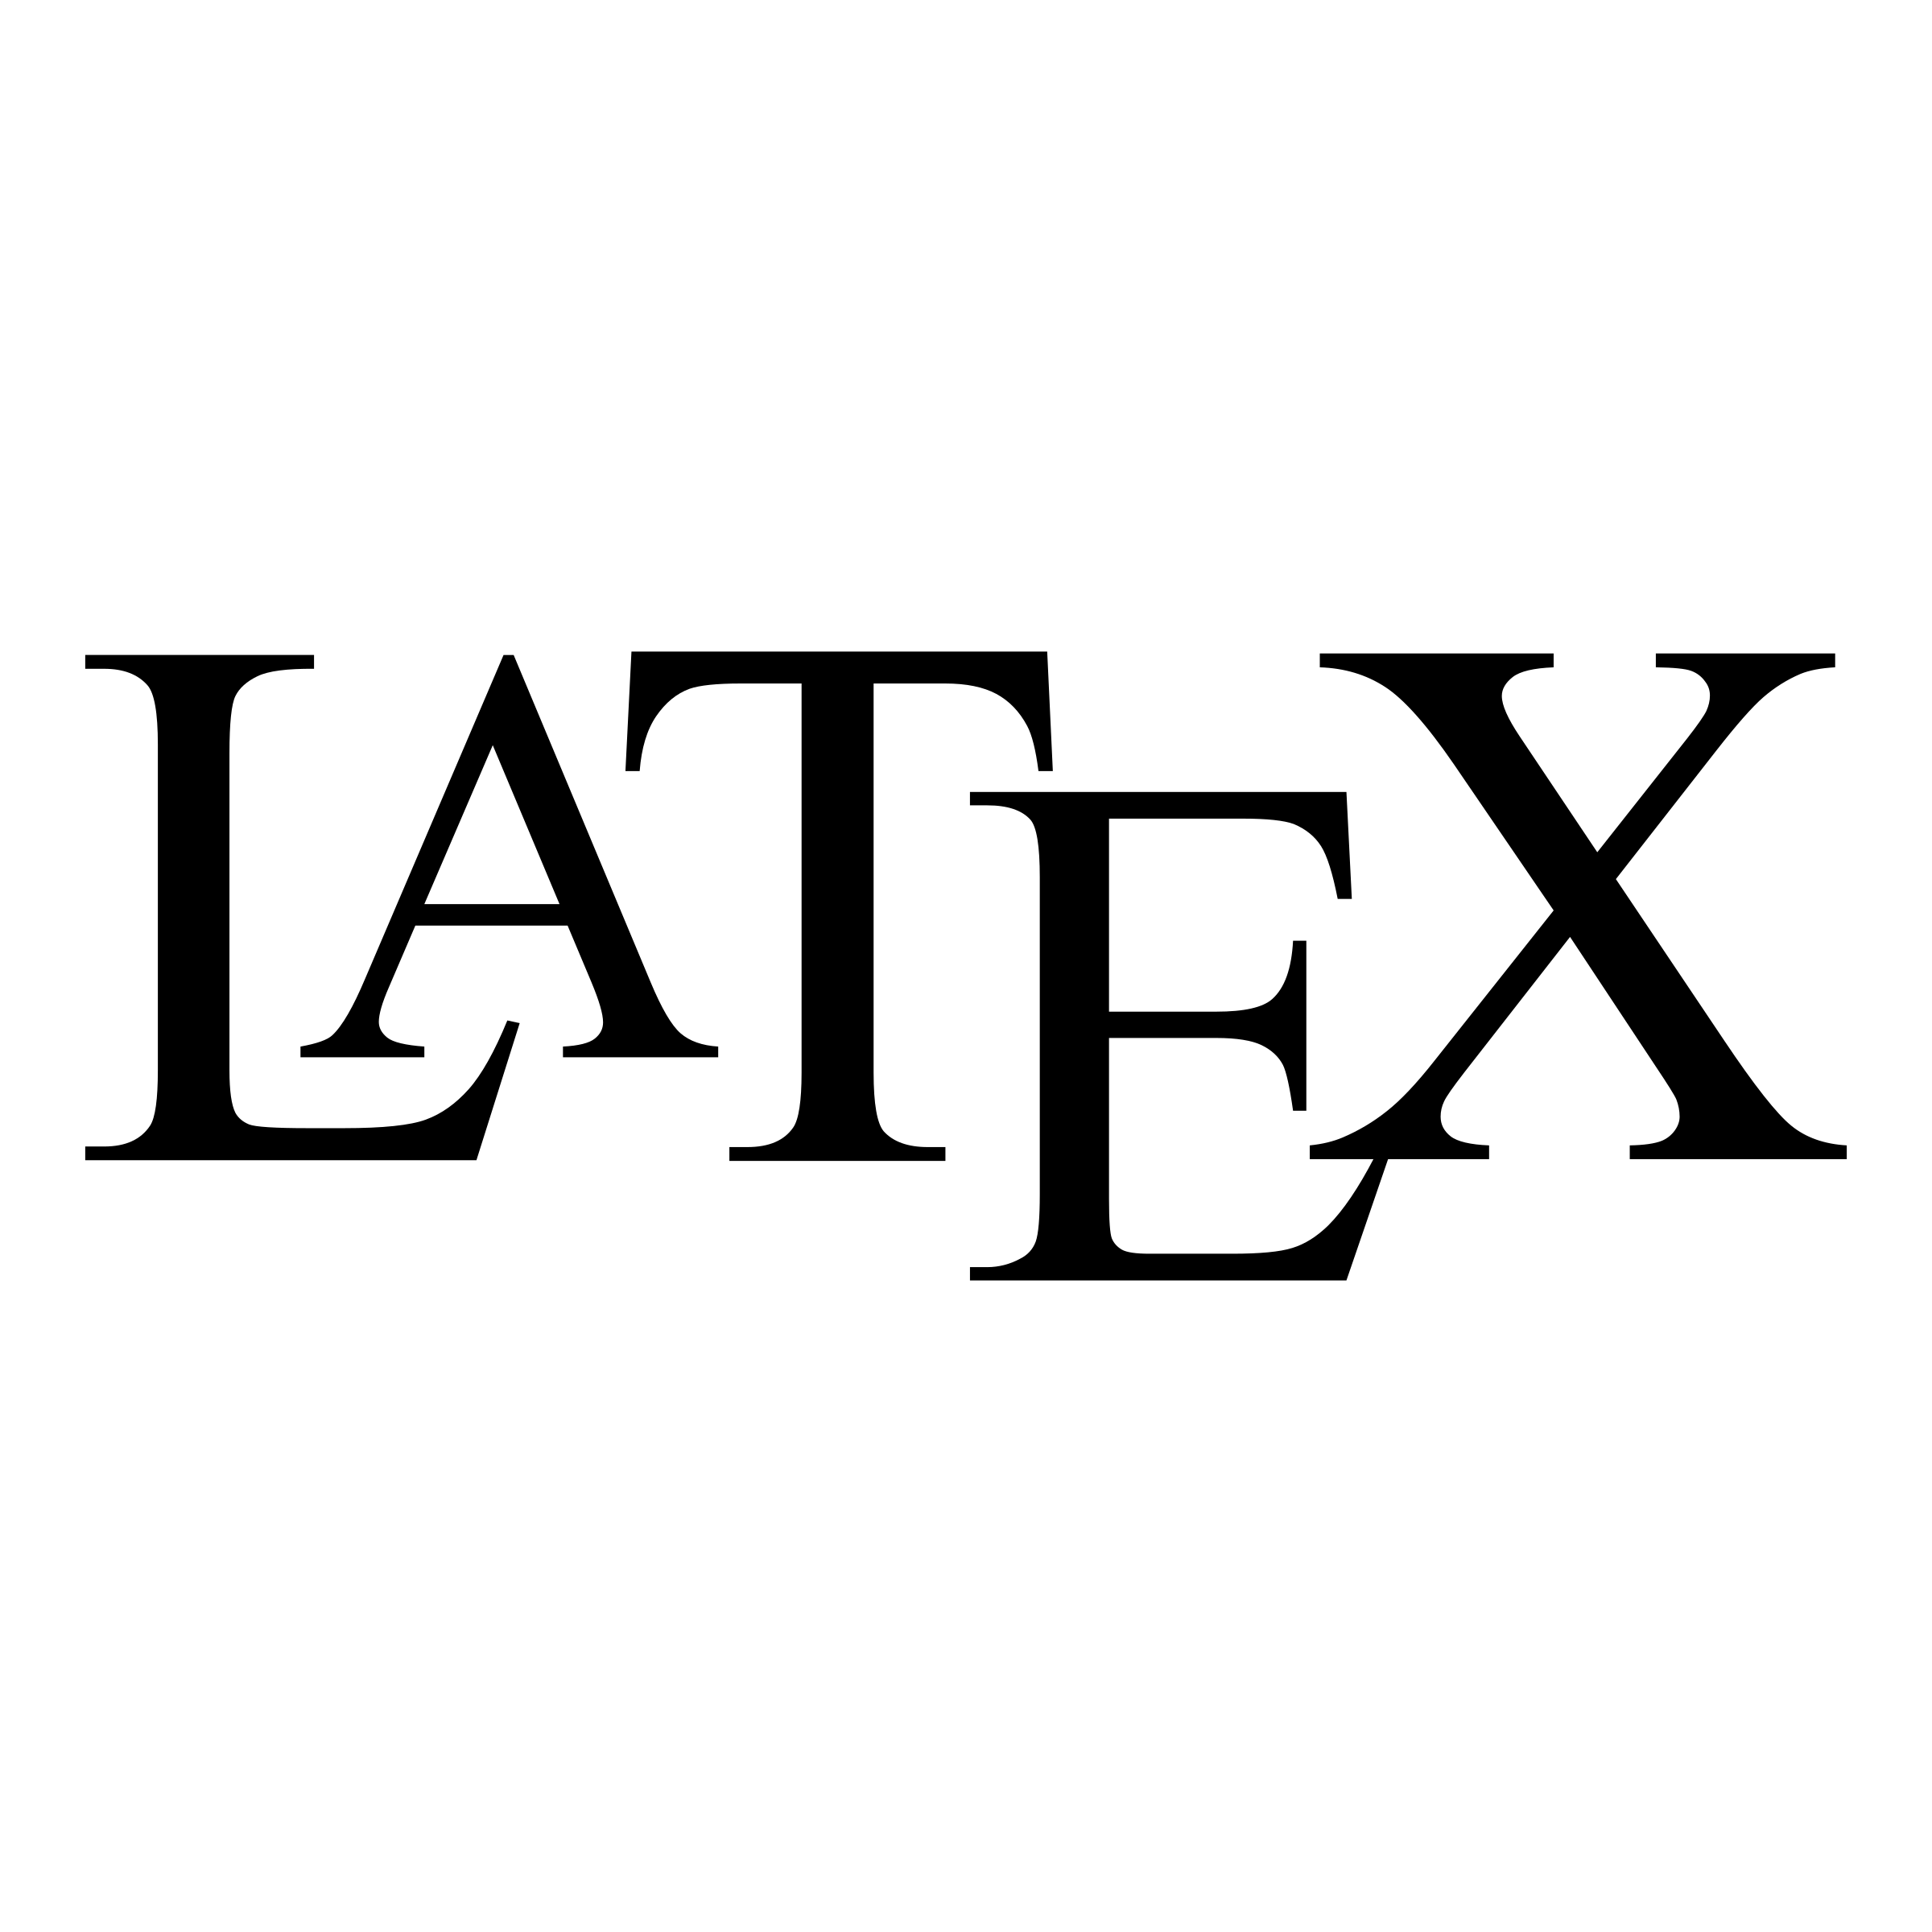
\includegraphics[width=0.4\textwidth]{LatexLogo.png}
        \caption{Title For Right}
    \end{subfigure}
\end{figure}

\subsubsection{Figure Arounded By Words}
\begin{figwindow}[2, r, 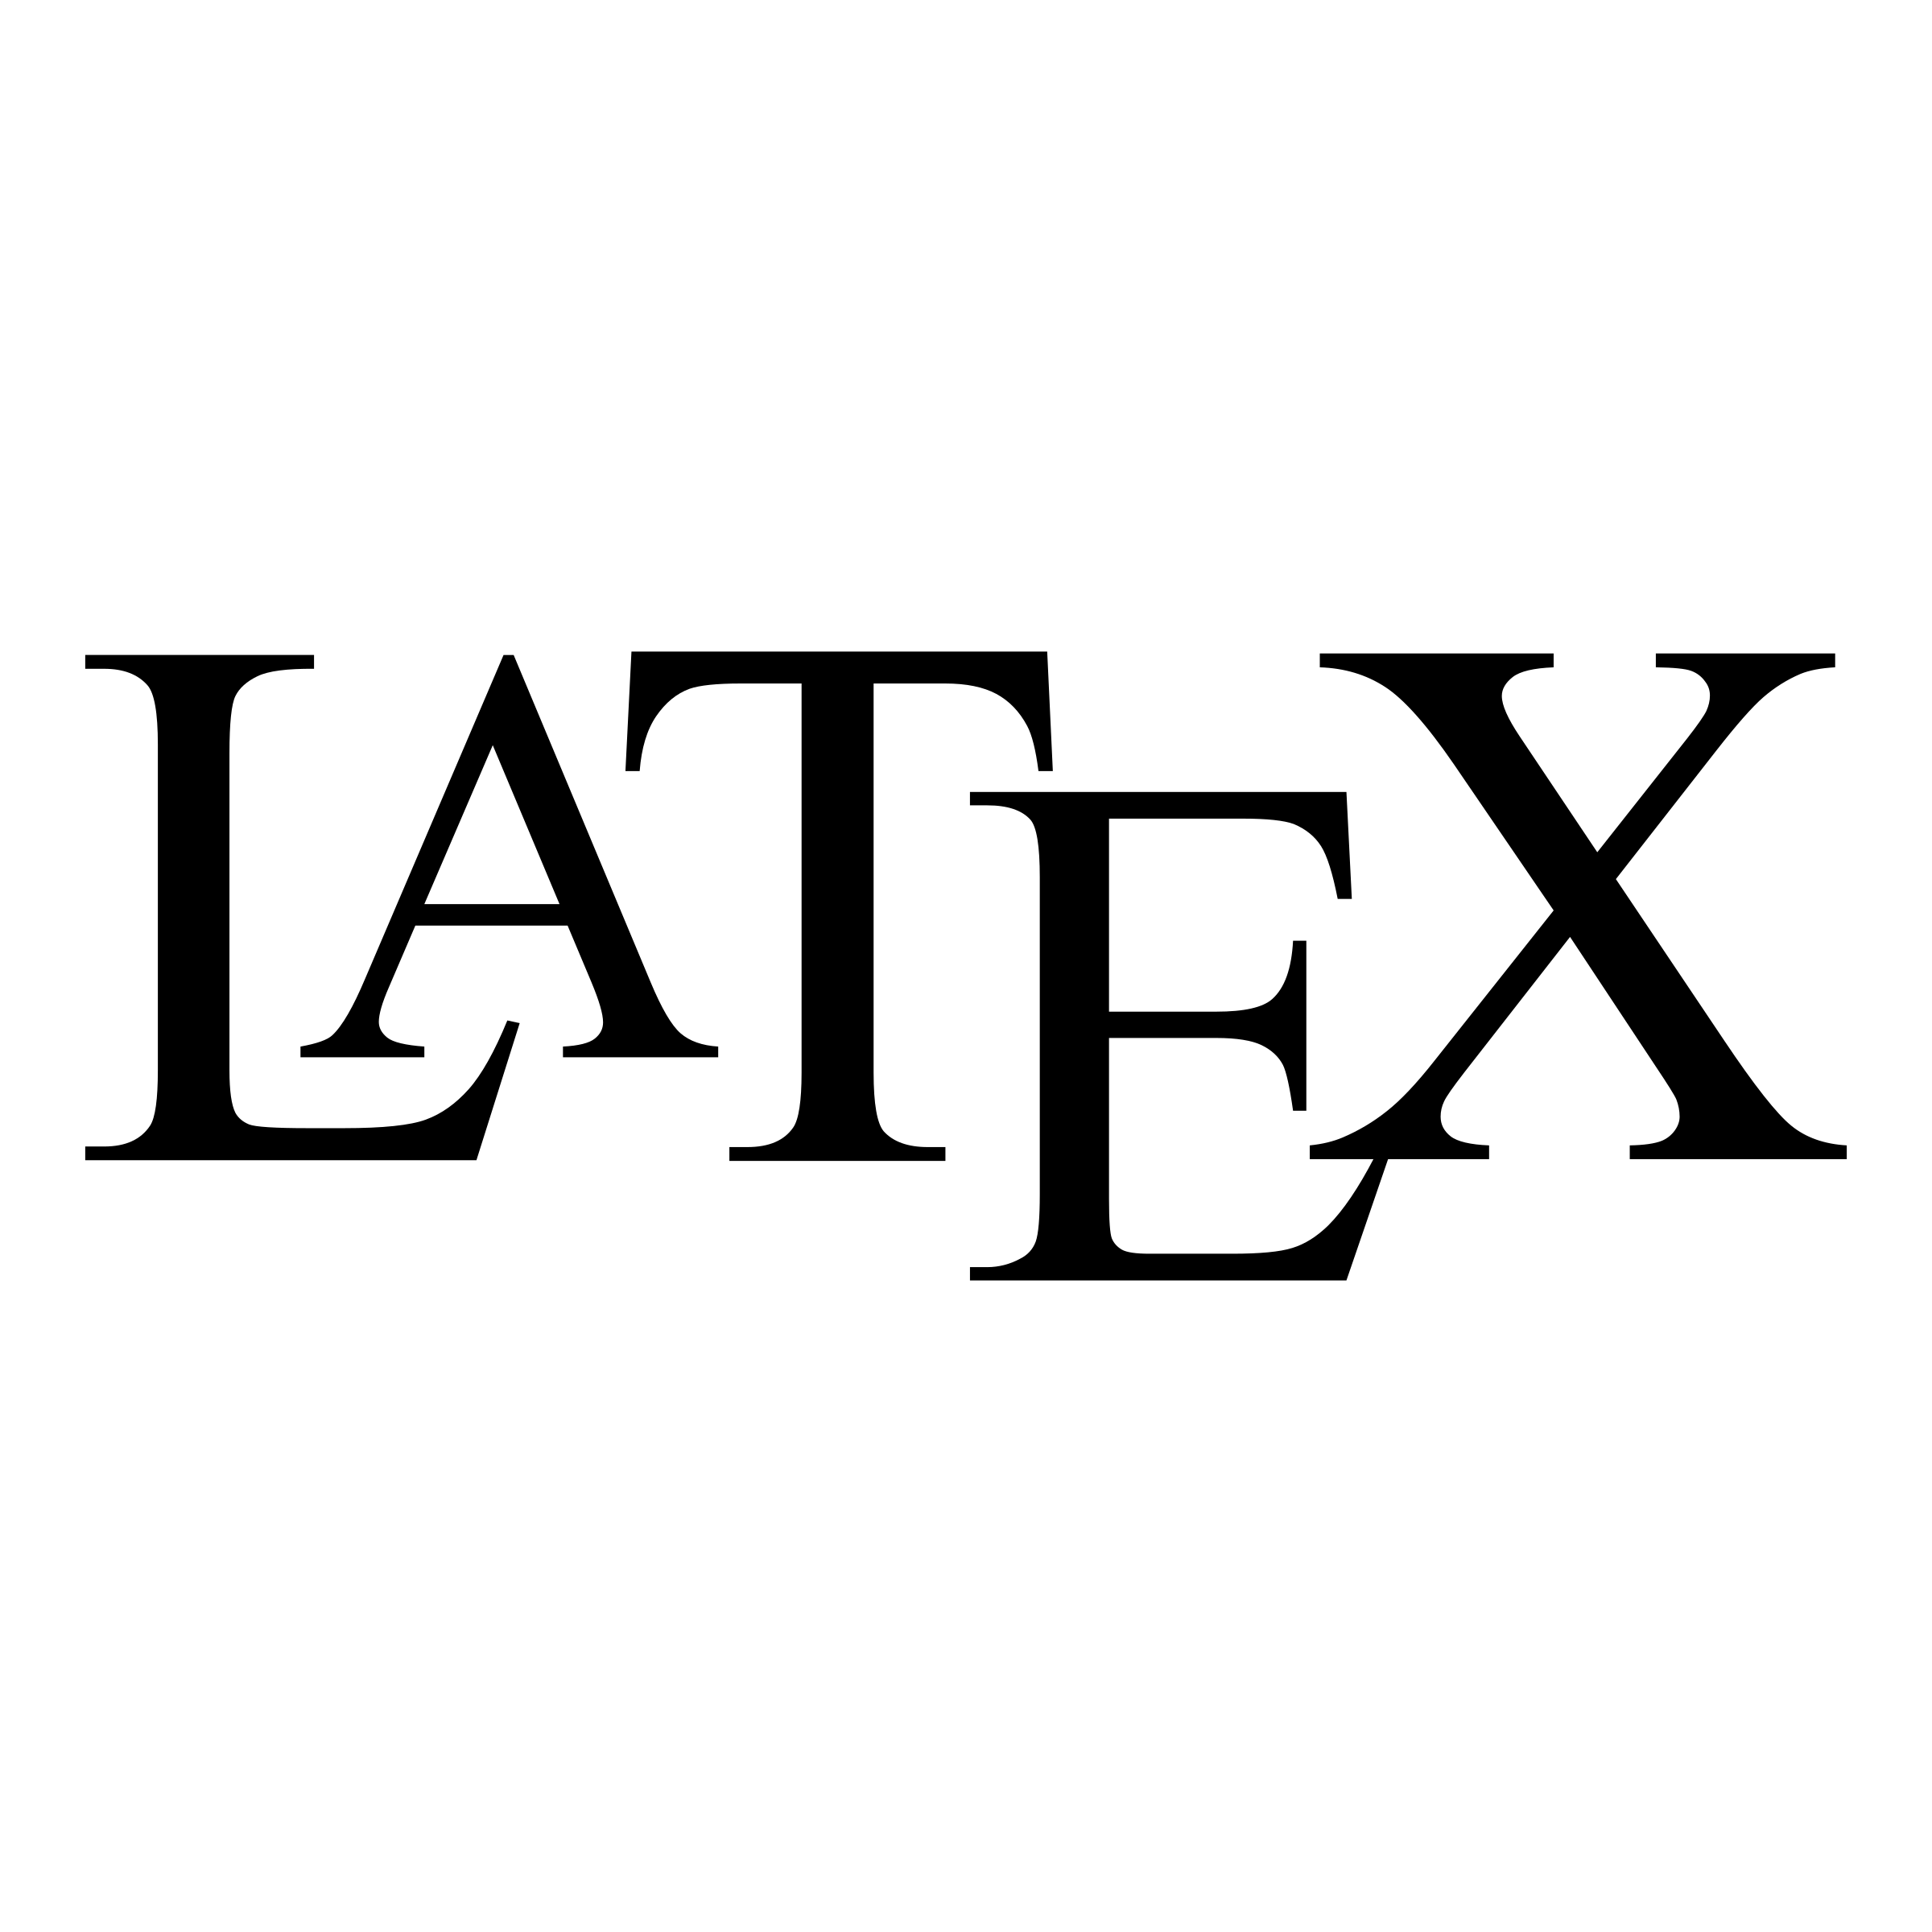
\includegraphics[scale=0.05]{LatexLogo.png}, Title Of Arounded Figure]      % must usepackage picinpar
    % bug exists
    These are the words around the figure, and the figure will appear below two lines, 
    lying in the right of the words, rather than left. The following will be fillings. 
    Hello world. Hello world. Hello world. Hello world. Hello world. Hello world. Hello world. 
    Hello world. Hello world. Hello world. Hello world. Hello world. Hello world. Hello world. 
    Hello world. Hello world. Hello world. Hello world. Hello world. Hello world. Hello world. 
    Hello world. Hello world. Hello world. Hello world. Hello world. Hello world. Hello world. 
    Hello world. Hello world. Hello world. Hello world. Hello world. Hello world. Hello world. 
    Hello world. Hello world. Hello world. Hello world. Hello world. Hello world. Hello world. 
    Hello world. Hello world. Hello world. Hello world. Hello world. Hello world. Hello world. 
    Hello world. Hello world. Hello world. Hello world. Hello world. Hello world. Hello world. 
    Hello world. Hello world. Hello world. Hello world. Hello world. Hello world. Hello world. 
    Hello world. Hello world. Hello world. Hello world. Hello world. Hello world. Hello world.
\end{figwindow}

\begin{wrapfigure}[10]{r}[1.5cm]{5cm}
    \centering
    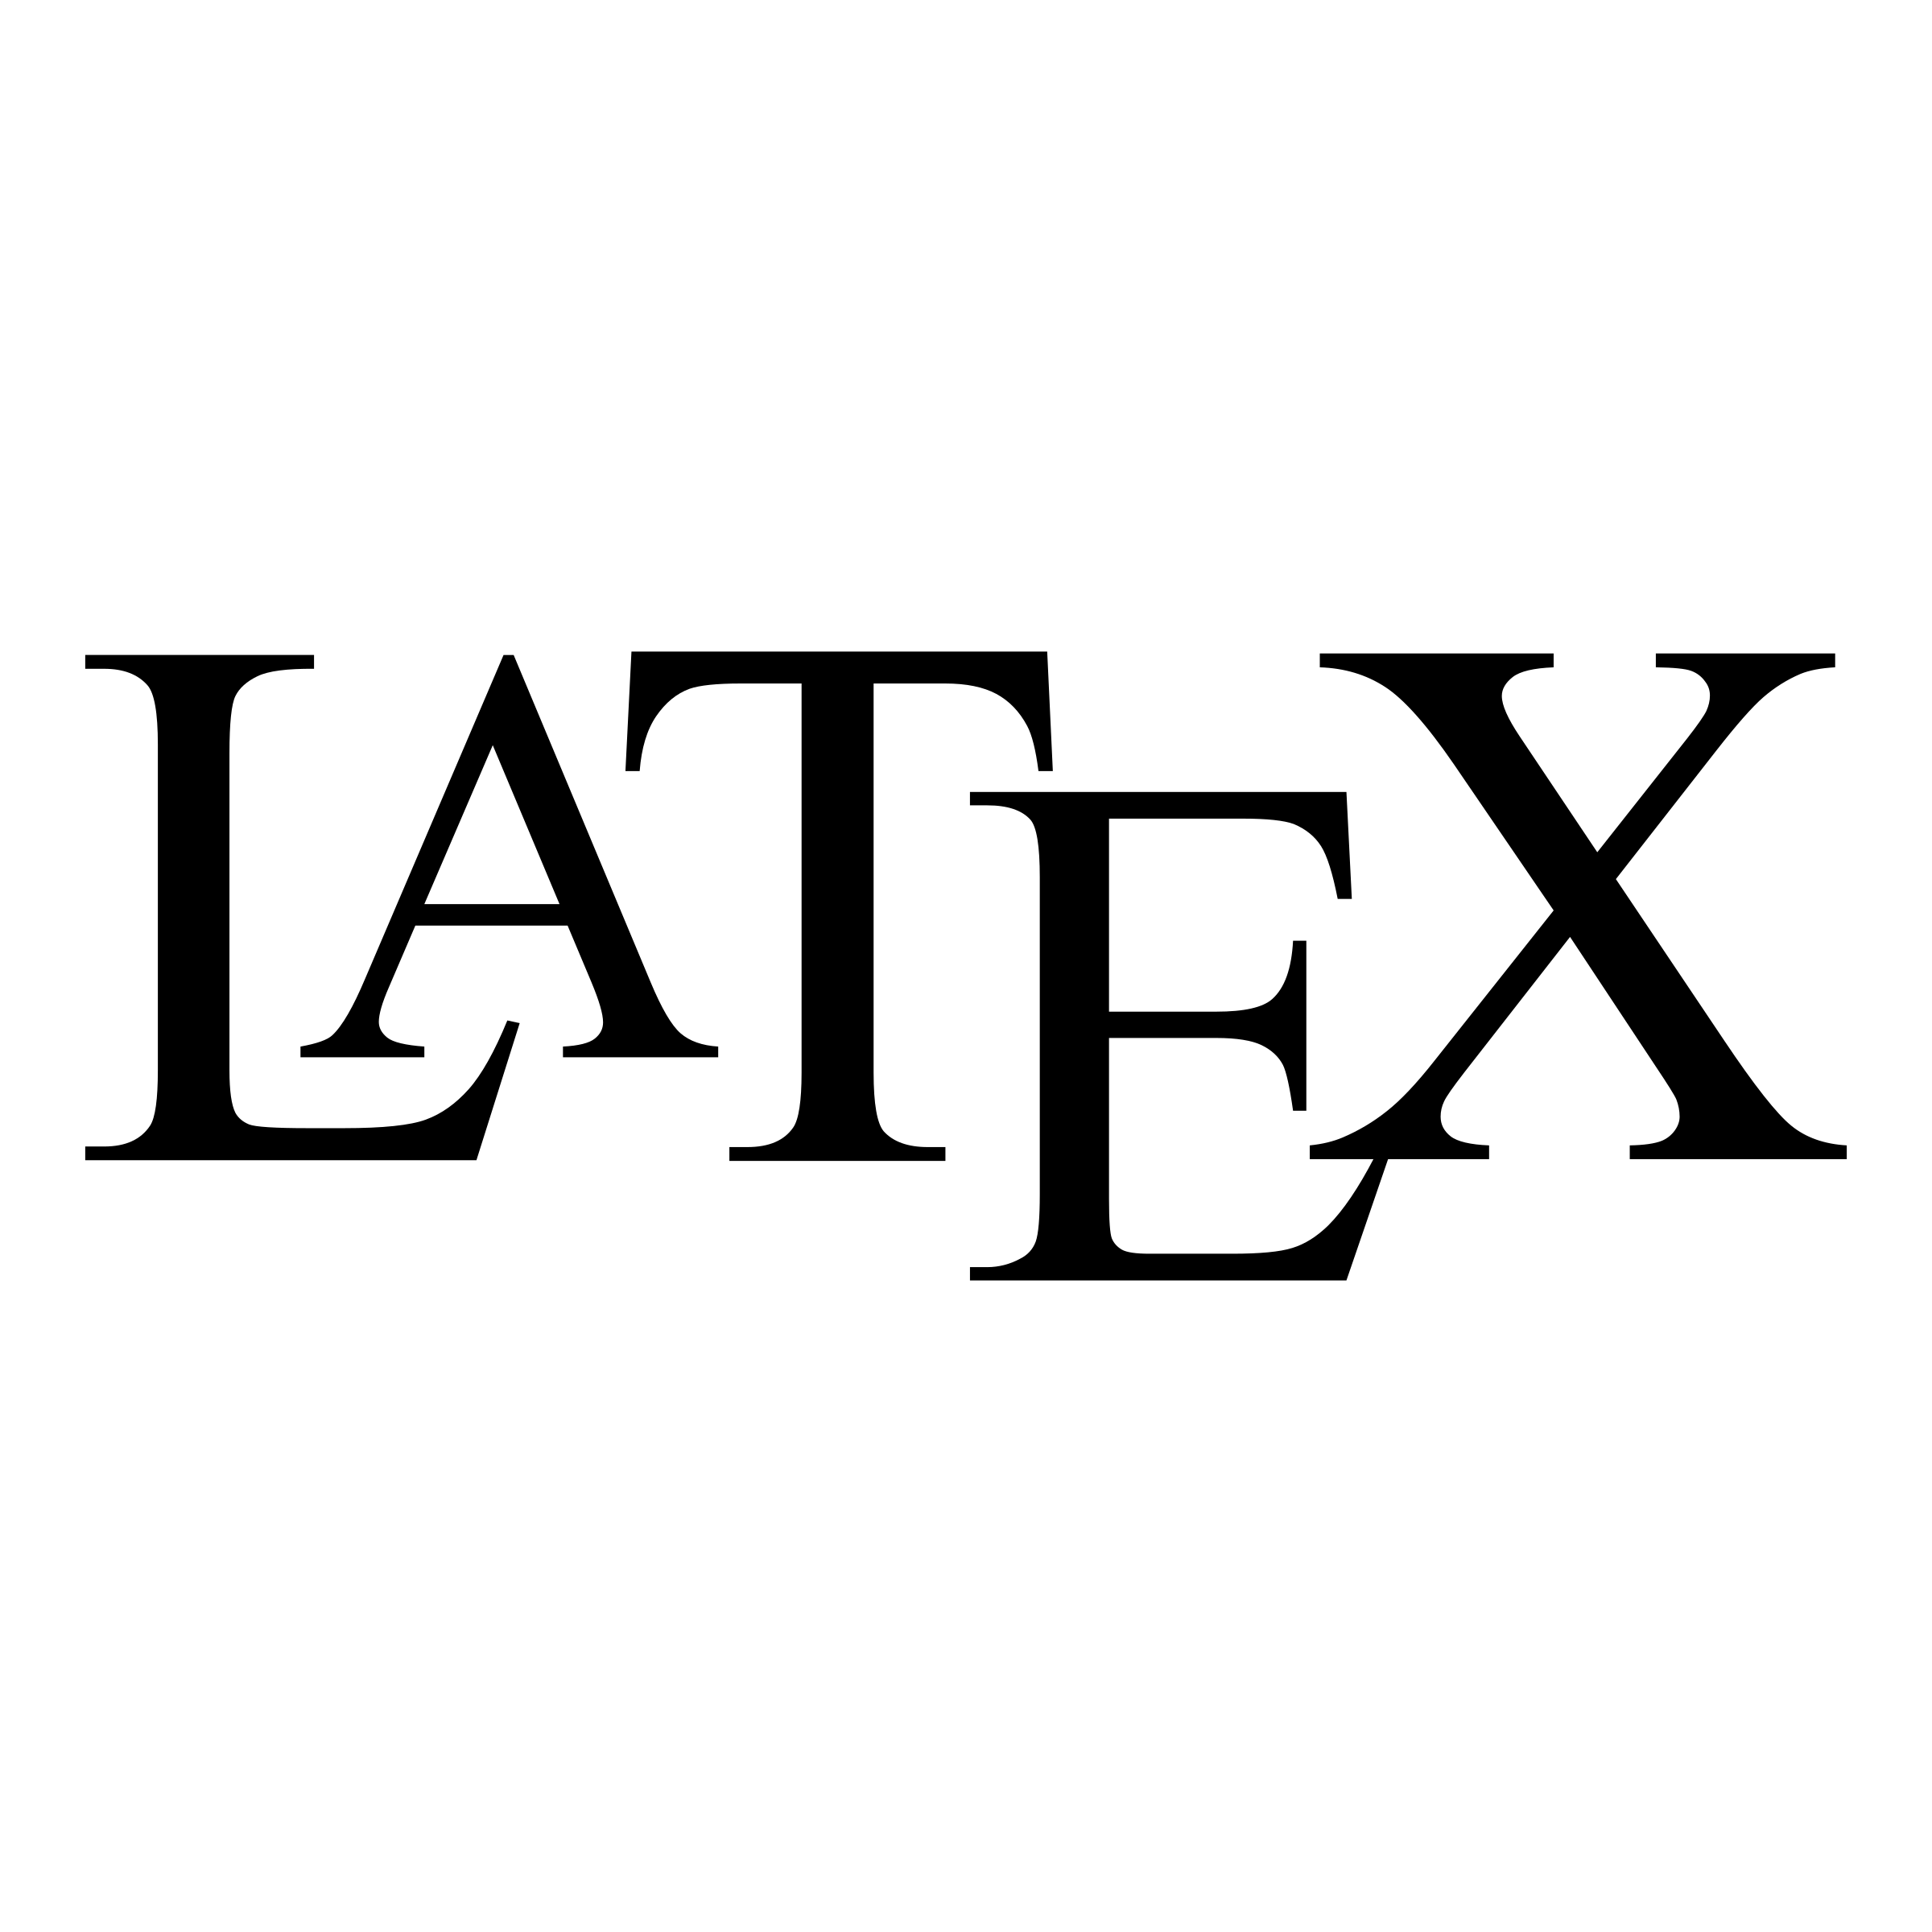
\includegraphics[scale=0.04]{LatexLogo.png}
    \caption{Title Of Arounded Figure}
\end{wrapfigure}
These are the words around the figure, and the figure will appear with height of 10 lines, 
lying in the right of the words, rather than left, and it will extend out 1.5cm, and has width of 5cm. 
The following will be fillings. 
Hello world. Hello world. Hello world. Hello world. Hello world. Hello world. Hello world. 
Hello world. Hello world. Hello world. Hello world. Hello world. Hello world. Hello world. 
Hello world. Hello world. Hello world. Hello world. Hello world. Hello world. Hello world. 
Hello world. Hello world. Hello world. Hello world. Hello world. Hello world. Hello world. 
Hello world. Hello world. Hello world. Hello world. Hello world. Hello world. Hello world. 
Hello world. Hello world. Hello world. Hello world. Hello world. Hello world. Hello world. 
Hello world. Hello world. Hello world. Hello world. Hello world. Hello world. Hello world. 
Hello world. Hello world. Hello world. Hello world. Hello world. Hello world. Hello world. 
Hello world. Hello world. Hello world. Hello world. Hello world. Hello world. Hello world. 
Hello world. Hello world. Hello world. Hello world. Hello world. Hello world. Hello world.

\subsubsection{General Float Control}
\begin{myfloat}                 % must newfloat myfloat
    \centering
    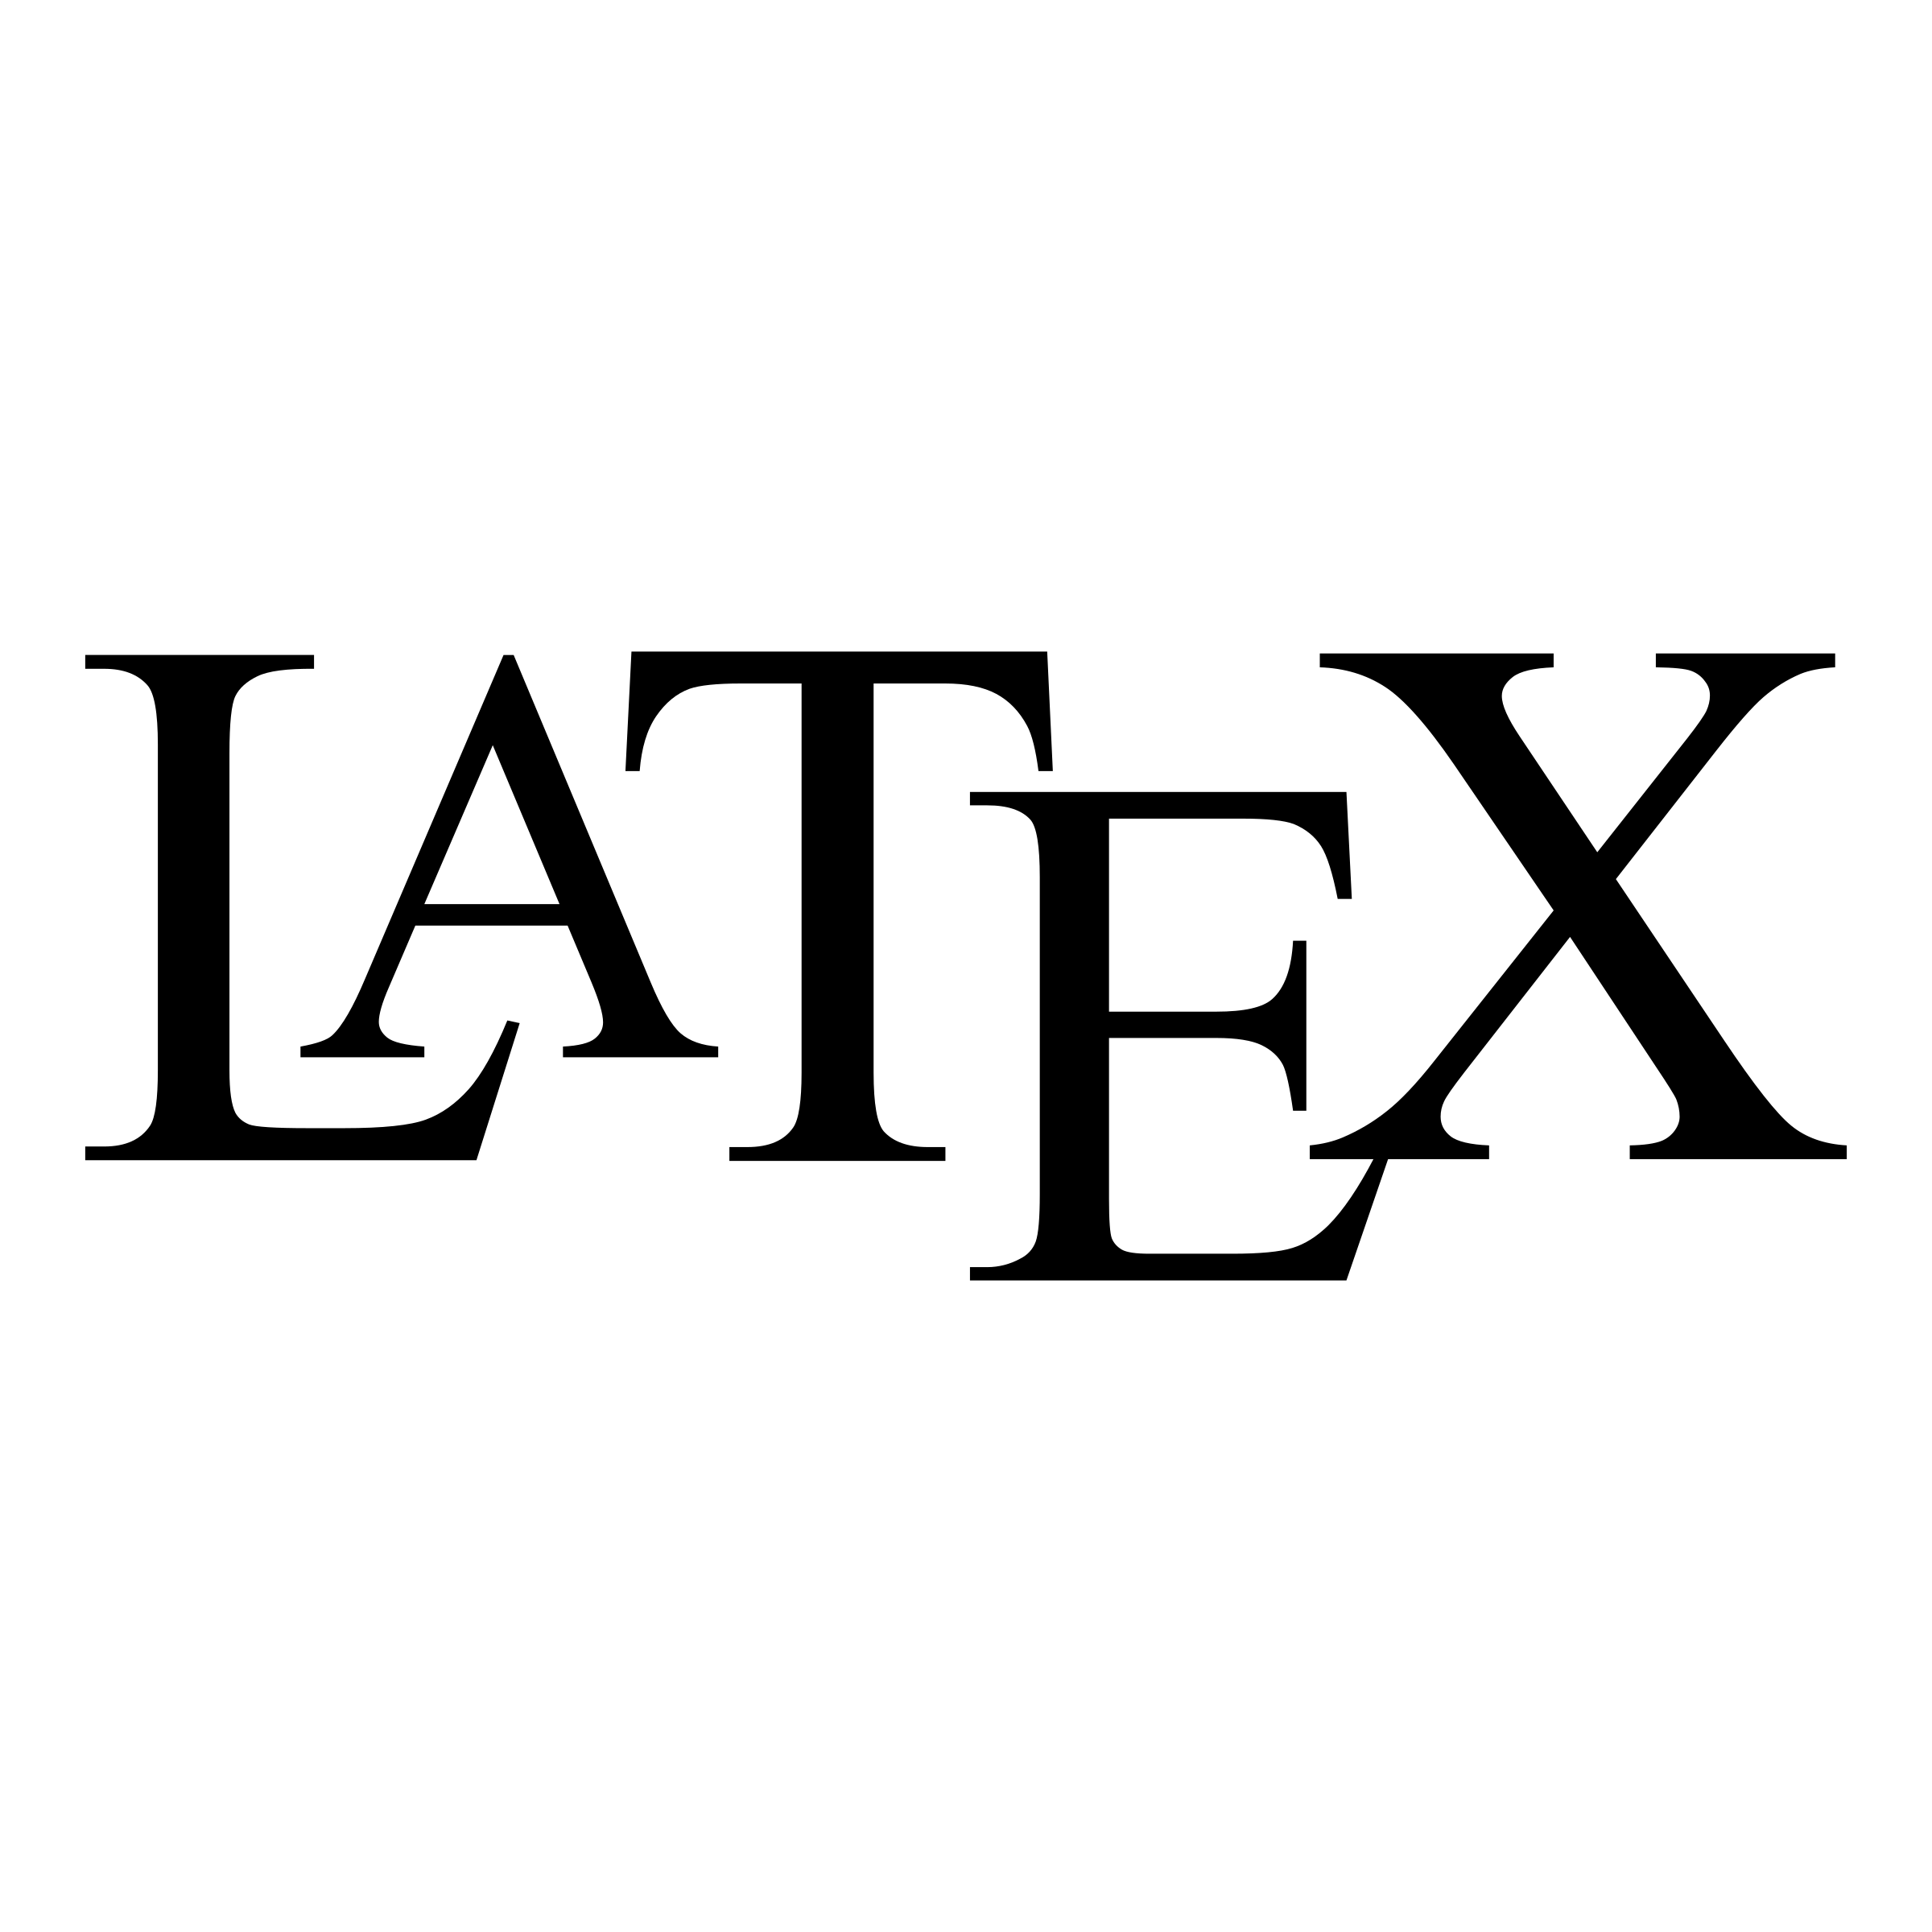
\includegraphics[scale=0.1]{LatexLogo.png}
    \caption{Figure In myfloat}
\end{myfloat}

\begin{mynewfloat}              % must DeclareFloatingEnvironment mynewfloat
    \centering
    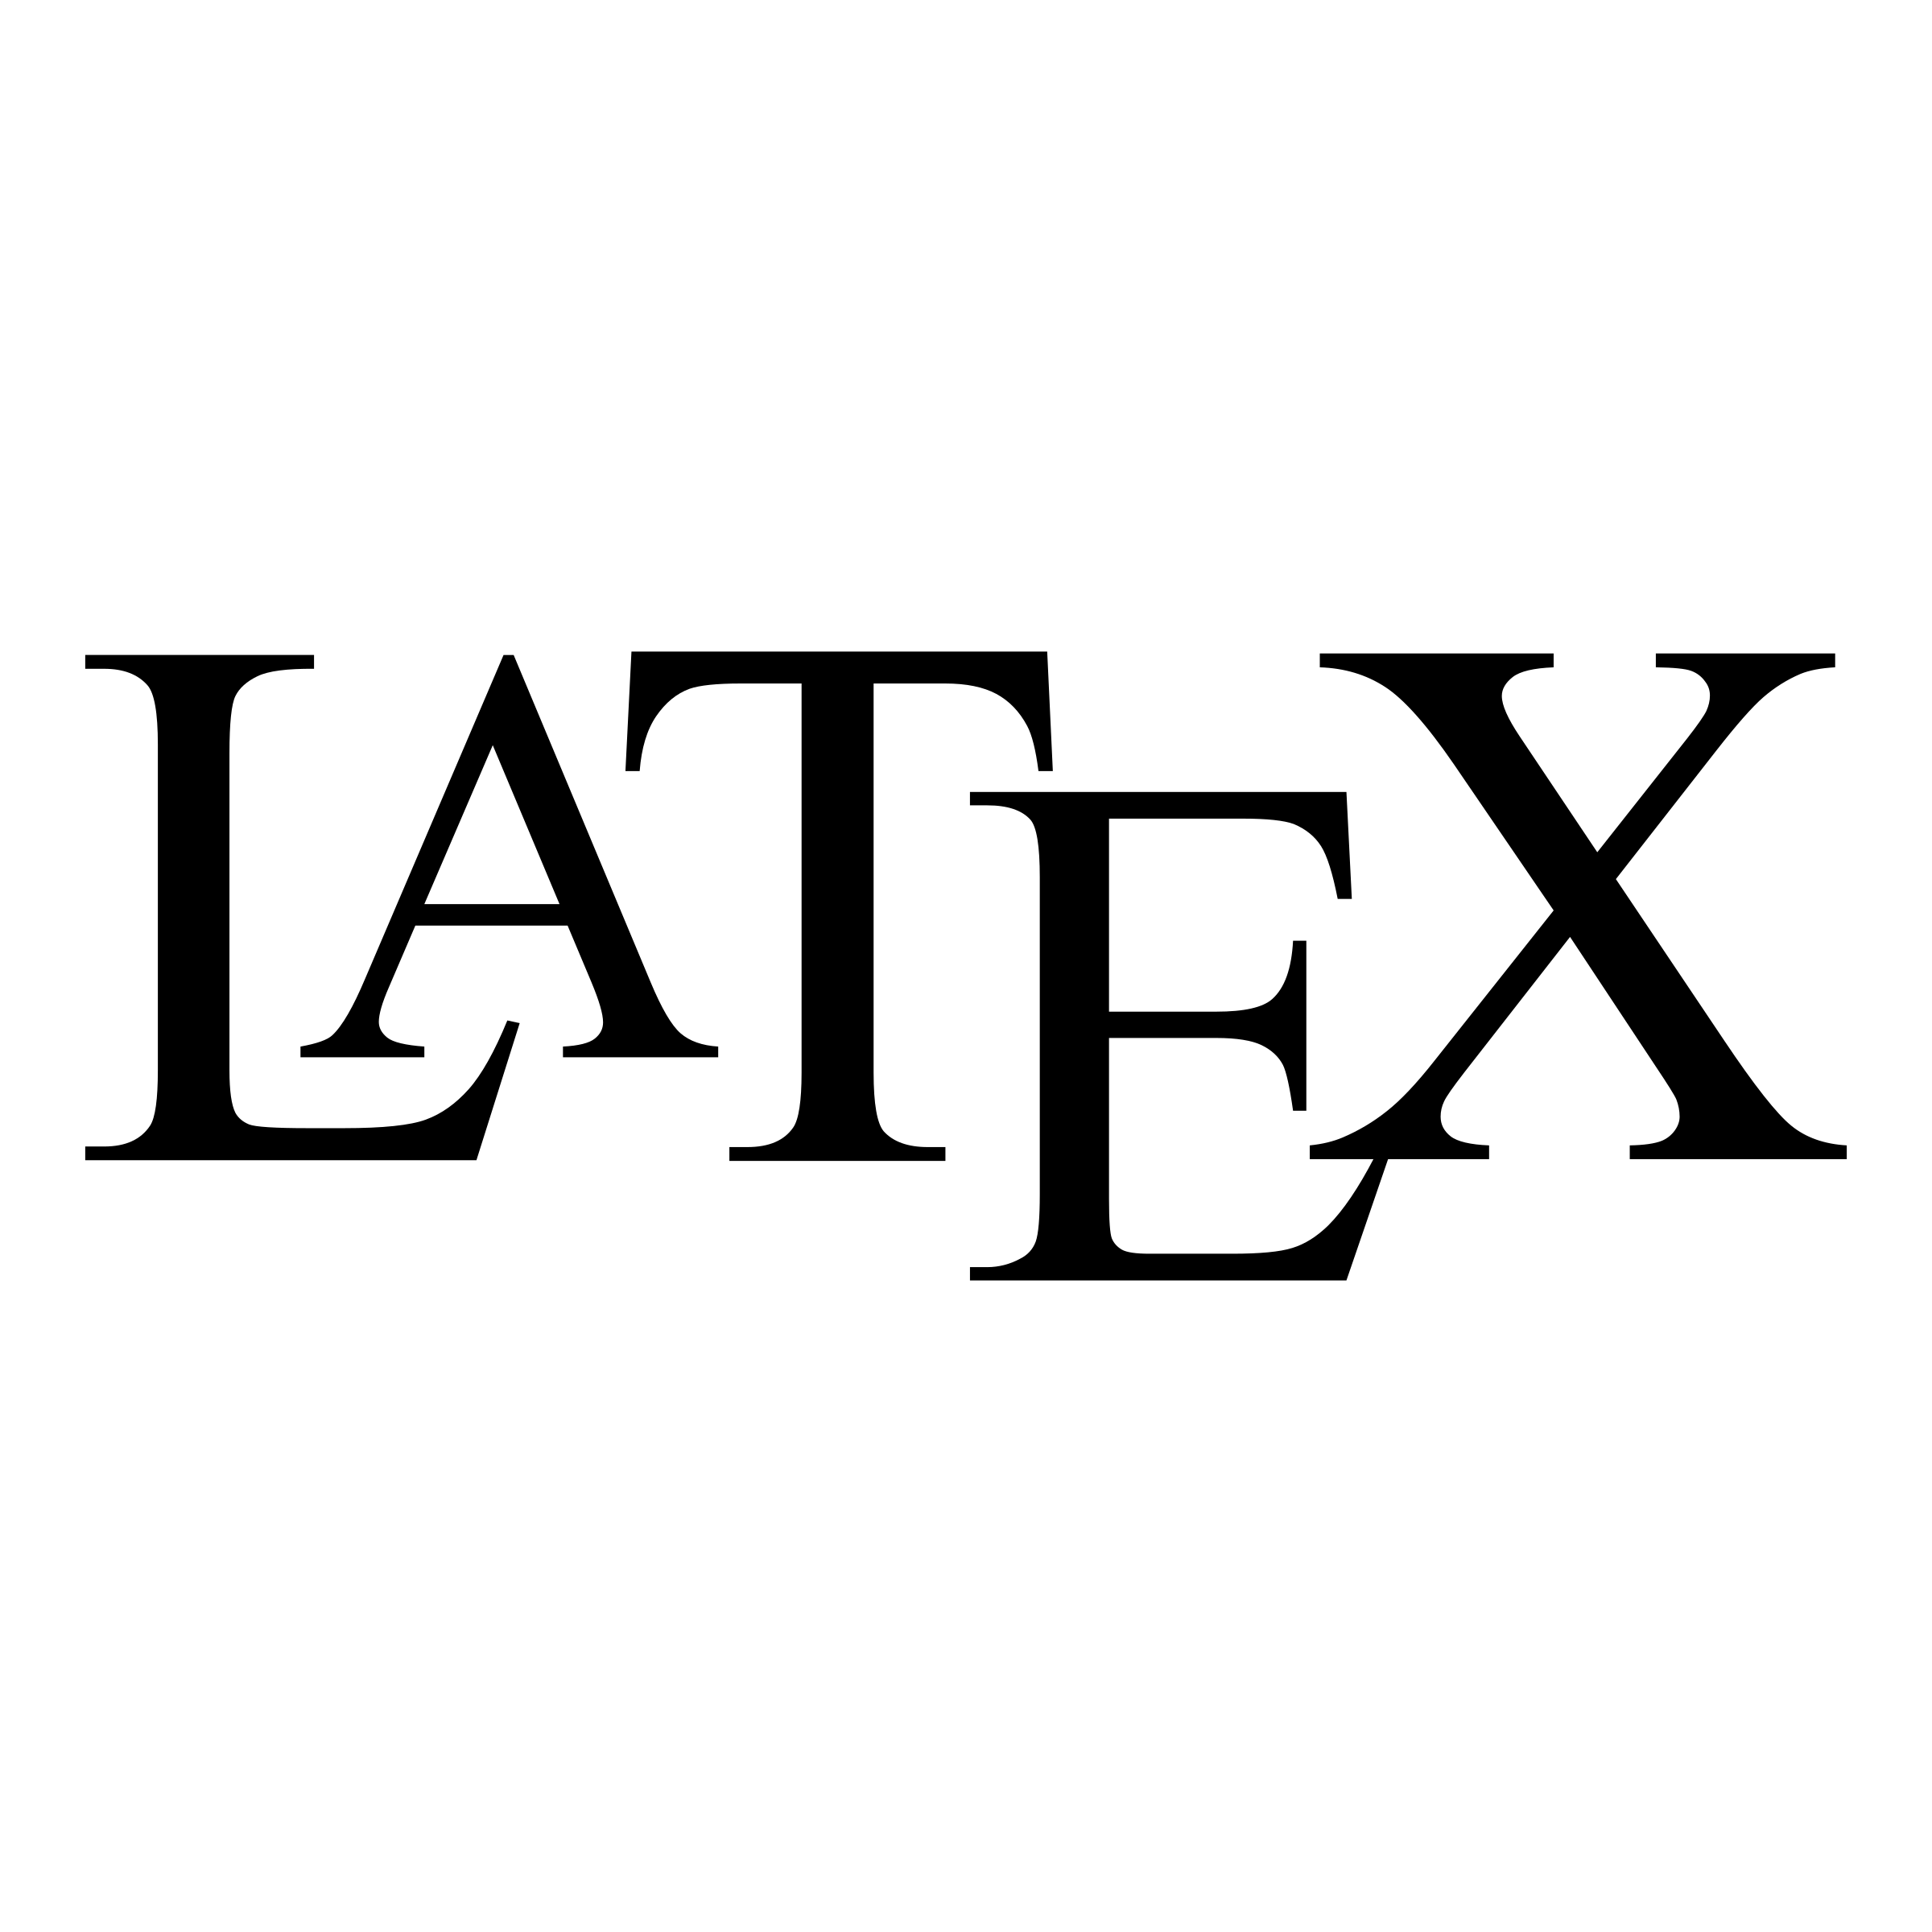
\includegraphics[scale=0.1]{LatexLogo.png}
    \caption{Figure In mynewfloat}
\end{mynewfloat}

\FloatBarrier                   % must usepackage placeins

\afterpage{\begin{figure}[H]
    \centering
    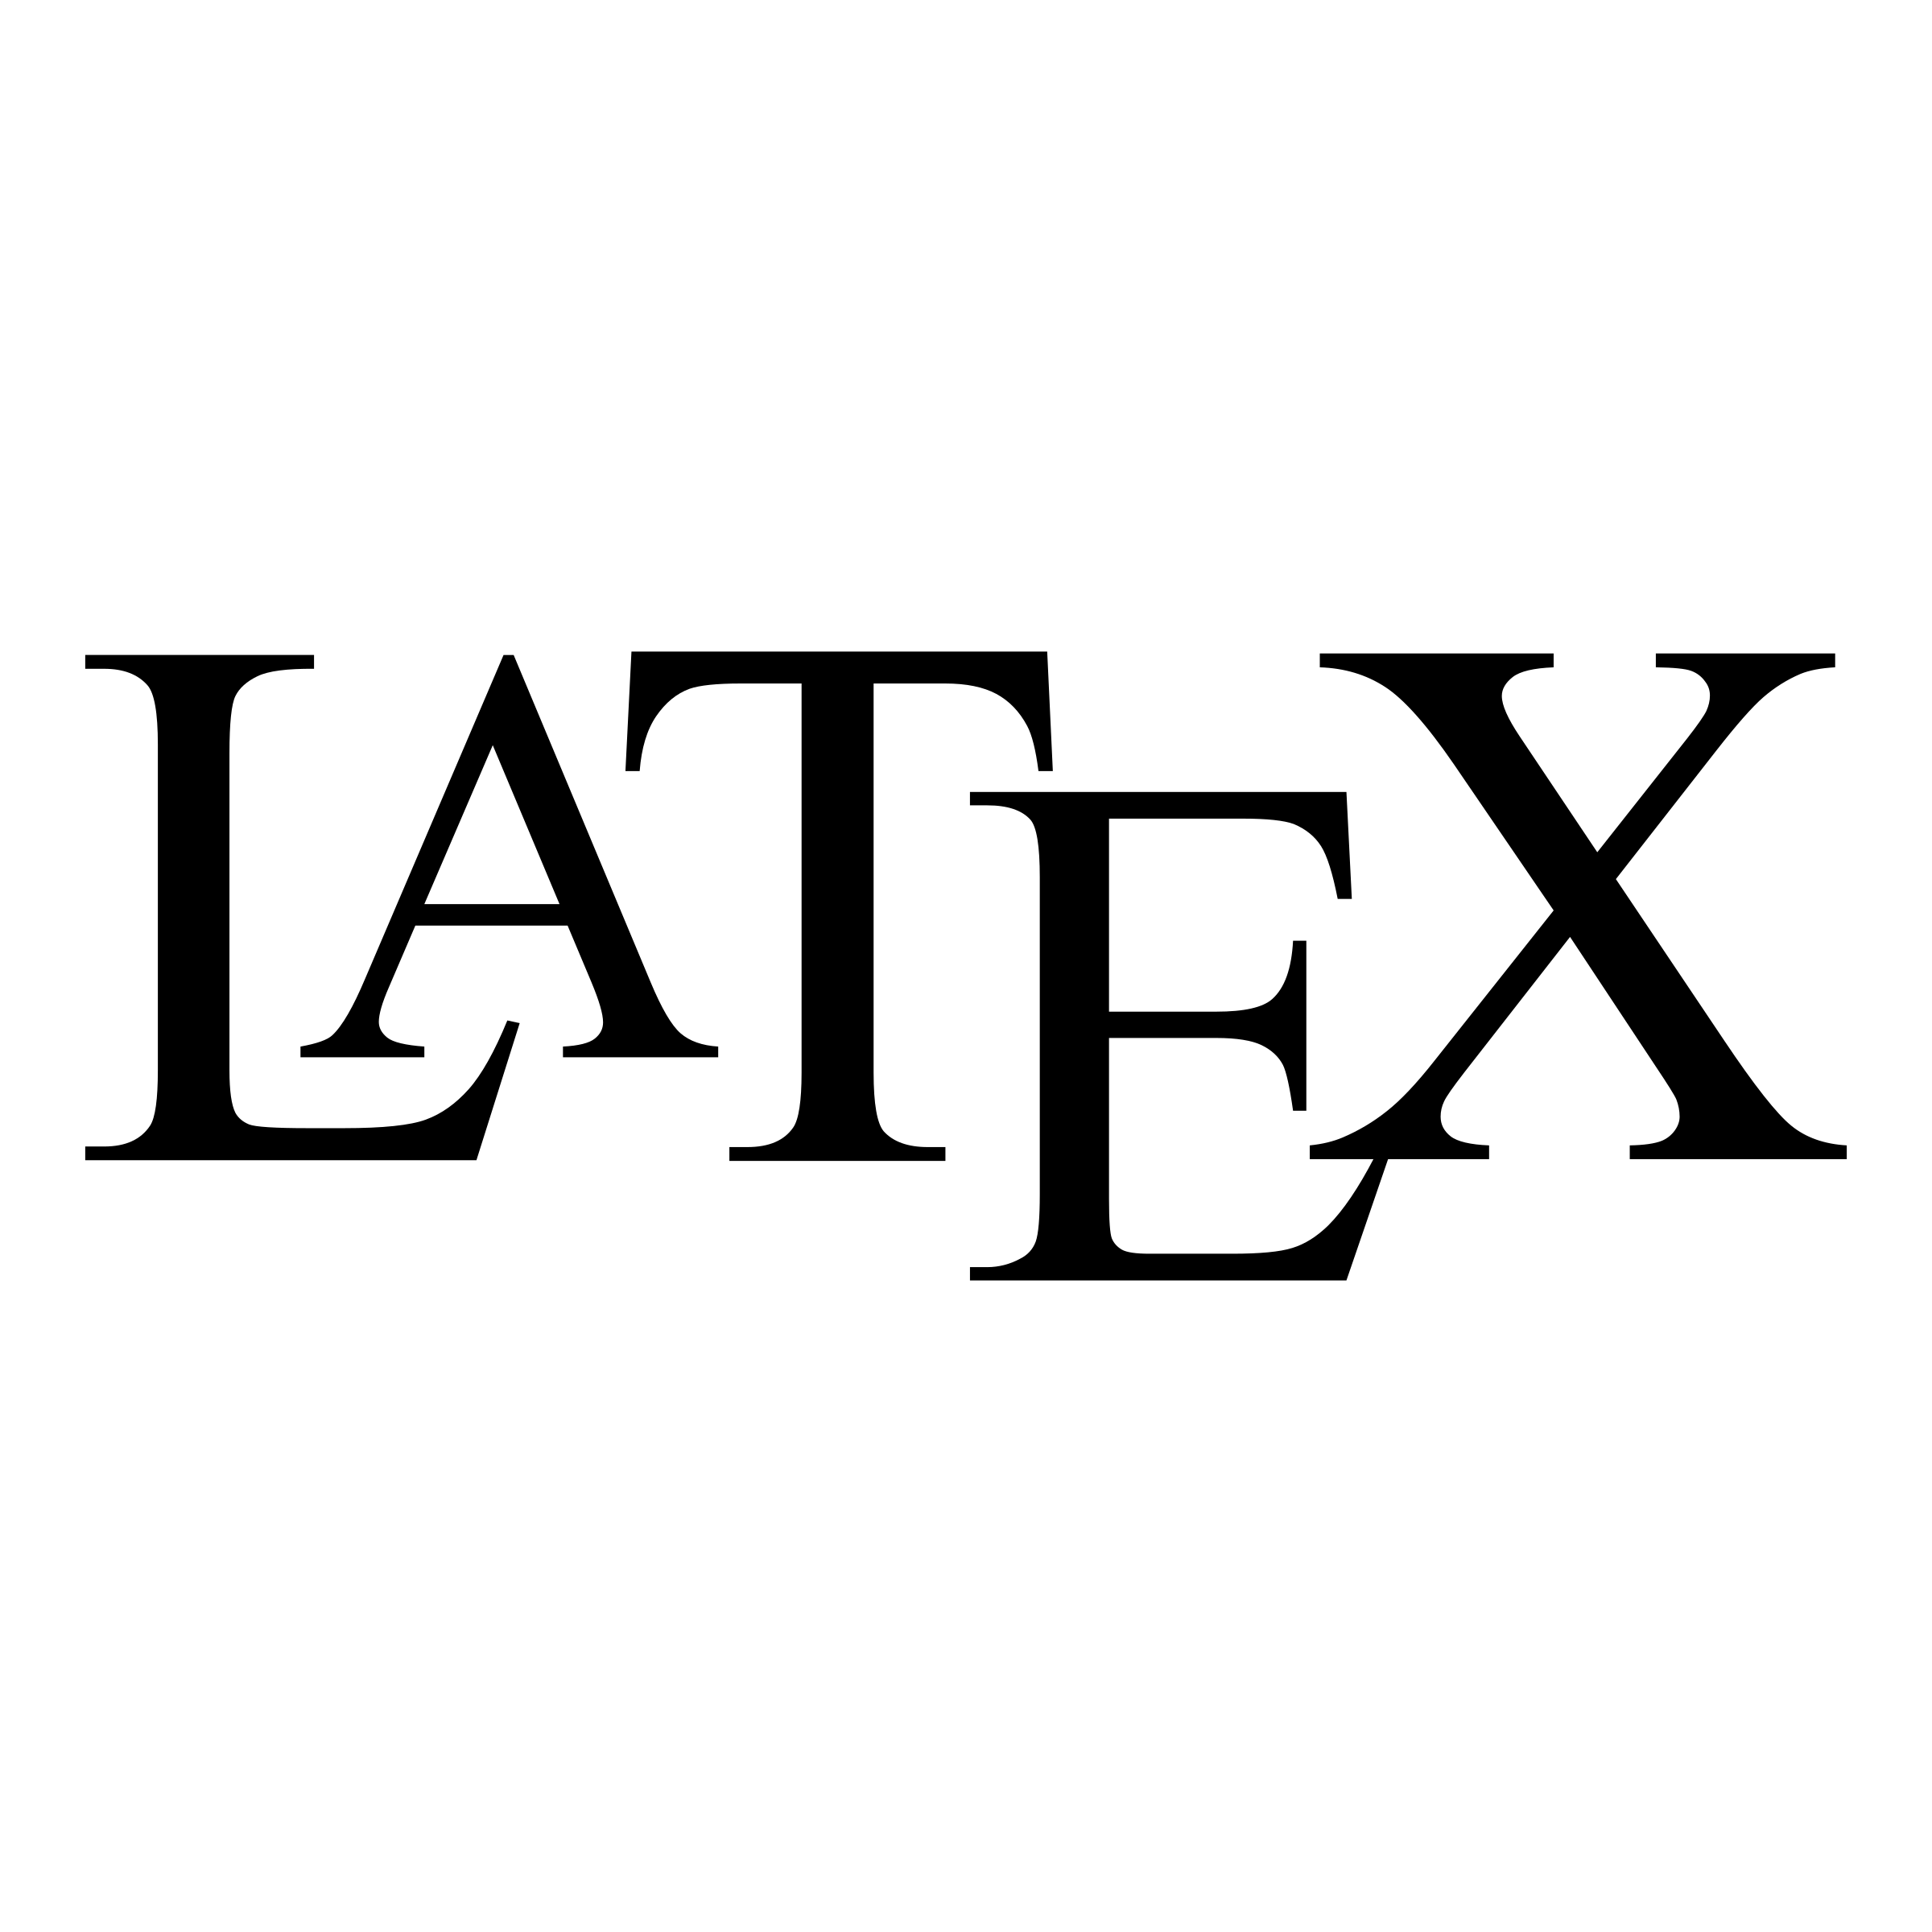
\includegraphics[scale=0.1]{LatexLogo.png}
    \caption{Figure In Top Of Next Page}
\end{figure}}

\subsection{Color}
% must usepackage xcolor
{
    \color{red}
    Red texts with \textcolor{blue}{blue words} texts.
}

% \pagecolor{cyan}

\colorbox{yellow}{Yellow box}

\fcolorbox{black}{green}{Black line green box}

\textcolor[gray]{0.5}{50\% gray text}, \textcolor[rgb]{0.6, 0.6, 0}{dark yellow text}, \textcolor[cmyk]{0.6, 0.6, 0, 0}{light purple text}

\textcolor{purple!70}{70\% purple text}, \textcolor{blue!60!black}{mixed blue and black text}, \textcolor{-red}{red complementary text}

\textcolor{darkred}{darkred text}       % must colorlet darkred

\subsection{Drawing}
\subsubsection{XY-pic}
% must usepackage xy
\begin{equation}
    \begin{gathered}
        \xymatrix{
            a & b & a+b \ar[ld]_{\alpha} \\
            1 & 2 \ar"1,1"^{\beta} & 3 \\
            \ar"1,1";"2,1"|{\gamma}
            \ar"1,2";"2,1"|\hole
        }
    \end{gathered}
\end{equation}

When $\xymatrix@1{A \ar[r]^{f} & B}$ in line text.
When $\xymatrix@1{A \ar[r]^>{f} & B}$ in line text.
When $\xymatrix@1{A \ar[r]^>>{f} & B}$ in line text.
When $\xymatrix@1{A \ar[r]^(0.6){f} & B}$ in line text.

When $\xymatrix@1{A \ar@{->}[r] & B}$ in line text.
When $\xymatrix@1{A \ar@{-->}[r] & B}$ in line text.
When $\xymatrix@1{A \ar@{=>}[r] & B}$ in line text.
When $\xymatrix@1{A \ar@{~>}[r] & B}$ in line text.
When $\xymatrix@1{A \ar@{.>}[r] & B}$ in line text.
When $\xymatrix@1{A \ar@{:>}[r] & B}$ in line text.
When $\xymatrix@1{A \ar@{-}[r] & B}$ in line text.
When $\xymatrix@1{A \ar@{}[r] & B}$ in line text.
When $\xymatrix@1{A \ar@{|->>}[r] & B}$ in line text.
When $\xymatrix@1{A \ar@{^(-_>}[r] & B}$ in line text.

When $\xymatrix@1{A \ar@/^/[r] & B}$ in line text.
When $\xymatrix@1{A \ar@/_/[r] & B}$ in line text.
When $\xymatrix@1{A \ar@(ur,dr) & B}$ in line text.

When $\xymatrix@1{A \ar@<0.5ex>[r] & \ar@<0.5ex>[l] B}$ in line text.

\begin{equation}
    \begin{gathered}
        \xymatrix@=2cm{% element separate length
            *[F]{A} \ar[r]^*+[F=]{m} & *-[o][F]{B} \\
            *[F.]{C} \ar[r]_*[F--]{n} & *[F-,]{D}
        }
    \end{gathered}
\end{equation}

\begin{equation}
    \begin{gathered}
        \xymatrix@L=1ex{% tag separate length
            \txt{Cat} \ar[r]^{f} & \txt{Dog}
        }
    \end{gathered}
\end{equation}

\begin{equation}
    \begin{gathered}
        \xymatrix@ru{% rotate
            A \ar[r] & B \ar[d] \\
            C \ar[u] & D \ar[l]
        }
    \end{gathered}
\end{equation}

\subsubsection{PSTricks}
% must usepackage pstricks or pstricks-add, bug exists
\begin{figure}[H]
    \centering
    \psset{unit=1.5cm}                                  % for setting coordinate unit
    \psset{linewidth=0.4pt}                             % for setting linewidth
    \psset{algebraic=true}                              % for using normal infix expression
    \begin{pspicture}(-3.5,-1.5)(4.5,1.5)
        \rput(-2,0){
            \psaxes[labels=none,ticks=none]{->}(0,0)(-1.2,-1.2)(1.2,1.2)
            \pscircle[linewidth=0.8pt](0,0){1}
            \pswedge[fillstyle=solid,fillcolor=gray,opacity=0.2](0,0){1}{0}{120}
            \pswedge[fillstyle=solid,fillcolor=gray,opacity=0.5](0,0){0.3}{0}{120}
            \uput[60](0.3;60){$120^{\circ}$}
            \pnode(1;120){P}
            \pnode(P|0,0){P0}
            \ncline{-}{P}{P0}
            \uput[120](P){$P$}
            \uput[d](P0){$P_0$}
        }

        \psaxes[labels=none,dx=1.57]{->}(0,0)(0,-1.2)(3.5,1.2)
        \psplot[linewidth=0.8pt]{0}{3.5}{sin(x)}
        \multido{\n=0+1.57,\i=0+90}{3}{
            \uput*[d](\n,0){\small$\i^{\circ}$}
        }
        \uput[r](*{3.5} {sin(x)}){$\sin x$}
        \pnode(!120 Pi mul 180 div 120 sin){Q}
        \pnode(Q|0,0){Q0}
        \uput[u](Q){$Q$}
        \uput[d](Q0){$Q_0$}
        \ncline{-}{Q}{Q0}

        \psline[linestyle=dashed](P)(Q)
    \end{pspicture}

    \caption{PSTricks Example}
\end{figure}

\subsubsection{TikZ}
% must usepackage tikz
\begin{figure}[H]
    \centering
    \begin{tikzpicture}[scale=1.5]
        \begin{scope}[xshift=-2cm]
            \draw[->] (-1.2,0) -- (1.2,0);
            \draw[->] (0,-1.2) -- (0,1.2);
            \draw[thick] (0,0) circle (1);
            \coordinate[label=120:$P$] (P) at (120:1);
            \coordinate[label=below:$P_0$] (P0) at (P |- 0,0);
            \draw (0,0) -- (P);
            \draw (P) -- (P0);
            \fill[fill=gray,fill opacity=0.2] (0,0) -- (0:1) arc (0:120:1) -- cycle;
            \filldraw[fill=gray, fill opacity=0.5] (0,0) -- (0:0.3) arc (0:120:0.3) -- cycle;
            \node[right] at (60:0.3) {$120^{\circ}$};
        \end{scope}

        \draw[->] (0,0) -- ({rad(210)}, 0);
        \draw[->] (0,-1.2) -- (0,1.2);
        \draw[thick,domain=0:rad(210)] plot (\x, {sin(\x r)}) node[right] {$\sin x$};
        \foreach \t in {0, 90, 180} {
            \draw ({rad(\t)}, -0.05) -- ({rad(\t)}, 0.05);
            \node[below, outer sep=2pt, fill=white, font=\small] at ({rad(\t)}, 0) {$\t^{\circ}$};
        }
        \foreach \y in {-1,1} {
            \draw (-0.05,\y) -- (0.05,\y);
        }
        \coordinate[label=above:$Q$] (Q) at ({rad(120)}, {sin(120)});
        \coordinate[label=below:$Q_0$] (Q0) at (Q |- 0,0);
        \draw (Q) -- (Q0);
        \draw[dashed] (P) -- (Q);
    \end{tikzpicture}

    \caption{TikZ Example}
\end{figure}

    \appendix
    \section{Appendix Section}
    This is the section of appendix.

    \bibliography{LiteratureReference.bib}      % for iterature reference generating

    \indexprologue{Index list 1 as follows.}    % for adding some additional description to index list
    \printindex[index1]                         % for printing the index list 1
    \indexprologue{Index list 2 as follows.}    % for adding some additional description to index list
    \printindex[index2]                         % for printing the index list 2

    % \printglossary                              % for printing the glossaries list, must usepackage glossaries
    
\end{document}

Here can comment without mark.